%% abtex2-modelo-trabalho-academico.tex, v-1.9.6 laurocesar
%% Copyright 2012-2016 by abnTeX2 group at http://www.abntex.net.br/ 
%%
%% This work may be distributed and/or modified under the
%% conditions of the LaTeX Project Public License, either version 1.3
%% of this license or (at your option) any later version.
%% The latest version of this license is in
%%   http://www.latex-project.org/lppl.txt
%% and version 1.3 or later is part of all distributions of LaTeX
%% version 2005/12/01 or later.
%%
%% This work has the L PPL maintenance status `maintained'.
%% 
%% The Current Maintainer of this work is the abnTeX2 team, led
%% by Lauro César Araujo. Further information are available on 
%% http://www.abntex.net.br/
%%
%% This work consists of the files abntex2-modelo-trabalho-academico.tex,
%% abntex2-modelo-include-comandos and abntex2-modelo-references.bib

% ---------------------------------------------------------------
% ---------------------------------------------------------------
% abnTeX2: Modelo de Trabalho Academico (tese de doutorado, dissertacao de
% mestrado e trabalhos monograficos em geral) em conformidade com 
% ABNT NBR 14724:2011: Informacao e documentacao - Trabalhos academicos -
% Apresentacao
% ---------------------------------------------------------------
% ---------------------------------------------------------------
% Personalização para o modelo Udesc 2020 7. ed. revisada e modificada
% MANUAL_2020_09_07_1599489825065_12510.pdf
% Autor: Felipe Joel Zimann (felipezimann@hotmail.com)
% Data: 02/12/2020 v1.0
% Data: 13/02/2021 v1.0.1 alterado tamanho numeração da página para 10pt
% ---------------------------------------------------------------
% ---------------------------------------------------------------

\documentclass[
	12pt,				% tamanho da fonte
	openright,			% capítulos começam em pág ímpar (insere página vazia caso preciso)
	oneside,			% para impressão em recto e verso (twoside). Oposto a (oneside)
	a4paper,			% tamanho do papel. 
	%hidelinks,
	chapter=TITLE,		% títulos de capítulos convertidos em letras maiúsculas
	section,
	%section=TITLE,		% títulos de seções convertidos em letras maiúsculas
	sumario=abnt-6027-2012,
	english,			% idioma adicional para hifenização
	brazil,				% o último idioma é o principal do documento
	%leqno,             % equações alinhadas a direita
	%fleqn,				% equações alinhadas a esquerda 
	]{abntex2}


% ----------------------------------------------------------
% Pacotes básicos 
% ----------------------------------------------------------
%\usetikzlibrary{arrows.meta, decorations.pathrend, matrix, positioning}
\usepackage{pdfpages}
\usepackage{graphicx}
\usepackage{subfigure}
\usepackage{subcaption} 
\usepackage{makecell}
\usepackage{fancyhdr} %pacote para inserção do nome do capitulo no cabeçalho

\usepackage{listings} %pacote para inserção de códigos
\lstdefinelanguage{JavaScript}{ % Definição da linguagem JavaScript
  keywords={break, case, catch, continue, debugger, default, delete, do, else,
    false, finally, for, function, if, in, instanceof, new, null, return,
    switch, this, throw, true, try, typeof, var, void, while, with, let, const},
  morecomment=[l]{//},
  morecomment=[s]{/*}{*/},
  morestring=[b]',
  morestring=[b]",
  sensitive=true
}
\lstset{
  language=JavaScript,
  basicstyle=\ttfamily\small,
  keywordstyle=\color{blue},
  commentstyle=\color{green!50!black},
  stringstyle=\color{red},
  numbers=left,
  numberstyle=\tiny,
  breaklines=true,
  frame=single,
  captionpos=b
}
\usepackage[noend]{algpseudocode}
\usepackage[portuguese,ruled,lined]{algorithm2e} % pacote para inserção de algoritmo 
%\usepackage[ruled,vlined]{algorithm2e}

\usepackage{amsmath}							% Pacote matemático
\usepackage{amssymb}							% Pacote matemático
\usepackage{amsfonts}							% Pacote matemático
%\usepackage{lmodern}							% Usa a fonte Latin Modern		
\usepackage{mathptmx} 							% Usa a fonte Times New Roman	 
\usepackage[T1]{fontenc}						% Seleção de códigos de fonte.
\usepackage[utf8]{inputenc}						% Codificação do documento (conversão automática dos acentos)
\usepackage{lastpage}							% Usado pela Ficha catalográfica
\usepackage{indentfirst}						% Indenta o primeiro parágrafo de cada seção.
\usepackage[dvipsnames,table]{xcolor}			% Controle das cores
\usepackage{graphicx}							% Inclusão de gráficos
\usepackage{microtype} 							% para melhorias de justificação
\usepackage{lipsum}								% para geração de dummy text
\usepackage[brazilian]{backref}	% Paginas com as citações na bibliografia
\usepackage[
  alf,
  abnt-emphasize=bf,
  abnt-full-initials=yes,
  abnt-etal-cite=3,
  abnt-etal-list=3,
  abnt-etal-text=it
]{abntex2cite}
%\usepackage[alf,abnt-emphasize=bf,abnt-full-initials=yes]{abntex2cite}					% Citações padrão ABNT
%\usepackage[num]{abntex2cite}					% Citações padrão ABNT numérica
\usepackage{adjustbox}							% Pacote de ajuste de boxes
\usepackage{subcaption}							% Inclusão de Subfiguras e sublegendas		
\usepackage{enumitem}							% Personalização de listas
\usepackage{siunitx}							% Grandezas e unidades
\usepackage[section]{placeins}					% Manter as figuras delimitadas na respectiva seção com a opção [section]


\usepackage{multirow}							% Multi colunas nas tabelas
\usepackage{array,tabularx} 					% Pacotes de tabelas
\usepackage{booktabs}							% Pacote de tabela profissional
\usepackage{rotating}							% Rotacionar figuras e tabelas
\usepackage{xfrac}								% Fazer frações n/d em linha
\usepackage{bm}									% Negrito em modo matemático
\usepackage{xstring}							% Manipulação de strings
\usepackage{pgfplots}							% Pacote de Gráficos
\usepackage{tikz}								% Pacote de Figuras
\usepackage[american, cuteinductors,smartlabels, fulldiode, siunitx, americanvoltages, oldvoltagedirection, smartlabels]{circuitikz}						% Pacote de circuitos elétricos
\usepackage{chemformula}						% Pacote para fórmulas químicas
\usepackage{chngcntr}							% Pacte usado para deixar numeração de equações sequencial 
%\counterwithout{equation}{chapter}
% fonte: https://latex.org/forum/viewtopic.php?t=15392

% Comando para deixar numeração das equações contínua (1), (2), (3)... ao invés de organizar por capítulos (1.1)(1.2)... (2.1)(2.2)
%\renewcommand{\theequation}{\arabic{equation}}

%\numberwithin{equation}{section}

% Cabecalho cabeçalho somente com numeração de página 10pt
\makepagestyle{PagNumReduzida}
\makeevenhead{PagNumReduzida}{\ABNTEXfontereduzida\thepage}{}{}
\makeoddhead{PagNumReduzida}{}{}{\ABNTEXfontereduzida\thepage}
%fonte: https://github.com/abntex/abntex2/wiki/HowToCustomizarCabecalhoRodape
%fonte: Manual memoir seção 7.3 pg. 111 pdf http://linorg.usp.br/CTAN/macros/latex/contrib/memoir/memman.pdf 

% Personalização das opções das listas
\setlist[itemize]{leftmargin=\parindent}

% Citação online --- MODIFICAR ---
\newcommand{\citeshort}[1]{\citeauthoronline{#1}~(\citeyear{#1})}

\newcommand{\me}[1]{Autor (#1).}

% Configuração do pgfplots
\pgfplotsset{compat=newest} %compat=1.14
\pgfplotsset{plot coordinates/math parser=false} 
\newlength\figureheight 
\newlength\figurewidth 


% Personalização das legendas
\usepackage[format = plain, %hang
			justification = centering,
			labelsep = endash,
			singlelinecheck = false,
			skip = 6pt,
			listformat = simple]{caption}	

% Personalização das unidades
\sisetup{output-decimal-marker = {,}}
\sisetup{exponent-product = \cdot, output-product = \cdot}
\sisetup{tight-spacing=true}
\sisetup{group-digits = false}

% Personalizações de tipo de colunas de tabelas
\newcolumntype{L}[1]{>{\raggedright\let\newline\\\arraybackslash\hspace{0pt}}m{#1}}
\newcolumntype{C}[1]{>{\centering\let\newline\\\arraybackslash\hspace{0pt}}m{#1}}
\newcolumntype{R}[1]{>{\raggedleft\let\newline\\\arraybackslash\hspace{0pt}}m{#1}}


% CONFIGURAÇÕES DE PACOTES
% Configurações do pacote backref
% Usado sem a opção hyperpageref de backref
\renewcommand{\backrefpagesname}{Citado na(s) página(s):~}
% Texto padrão antes do número das páginas
\renewcommand{\backref}{}
% Define os textos da citação
\renewcommand*{\backrefalt}[4]{
	\ifcase #1 %
	Nenhuma citação no texto.%
	\or
	Citado na página #2.%
	\else
	Citado #1 vezes nas páginas #2.%
	\fi}%

% alterando o aspecto da cor azul
\definecolor{blue}{RGB}{41,5,195}

% informações do PDF
\makeatletter
\hypersetup{
	%pagebackref=true,
	pdftitle={\@title}, 
	pdfauthor={\@author},
	pdfsubject={\imprimirpreambulo},
	pdfcreator={LaTeX with abnTeX2},
	pdfkeywords={abnt}{latex}{abntex}{abntex2}{trabalho academico}, 
	colorlinks=true,       		% false: boxed links; true: colored links
	linkcolor=black,          	% color of internal links
	citecolor=black,        	% color of links to bibliography
	filecolor=black,      		% color of file links
	urlcolor=black,
	bookmarksdepth=4
}


% ---
% Possibilita criação de Quadros e Lista de quadros.
% Ver https://github.com/abntex/abntex2/issues/176
%
\newcommand{\quadroname}{Quadro}
\newcommand{\listofquadrosname}{Lista de quadros}

\newfloat[chapter]{quadro}{loq}{\quadroname}
\newlistof{listofquadros}{loq}{\listofquadrosname}
\newlistentry{quadro}{loq}{0}

% configurações para atender às regras da ABNT
\setfloatadjustment{quadro}{\centering}
\counterwithout{quadro}{chapter}
\renewcommand{\cftquadroname}{\quadroname\space} 
\renewcommand*{\cftquadroaftersnum}{\hfill--\hfill}

\setfloatlocations{quadro}{hbtp} % Ver https://github.com/abntex/abntex2/issues/176
% ---


% Espaçamento depois do título
\setlength{\afterchapskip}{1.5\baselineskip}
% O tamanho do parágrafo é dado por:
\setlength{\parindent}{1.25cm}
% Controle do espaçamento entre um parágrafo e outro:
\setlength{\parskip}{0.25cm}  % tente também \onelineskip
%\SingleSpacing % Espaçamento simples 
\OnehalfSpacing % Espaçamento 1,5 (UDESC/CCT)
%\DoubleSpacing	% Espaçamento duplo

% ---
% Margens - NBR 14724/2011 - 5.1 Formato
% ---
\setlrmarginsandblock{3cm}{3cm}{*}
\setulmarginsandblock{2.5cm}{2.5cm}{*}
\checkandfixthelayout[fixed]
% ---


\usepackage{etoolbox}
\robustify\setcounter
\robustify\addtocounter
\robustify\setlength
\robustify\addtolength


% --------------------------------------------------------
% INICIO DAS CUSTOMIZAÇÕES PARA A UDESC
% --------------------------------------------------------

% --------------------------------------------------------
% Fontes padroes de part, chapter, section, subsection e subsubsection
% --------------------------------------------------------

% --- Chapter: NEGRITO + MAIÚSCULAS (abnTeX2 já aplica MakeUppercase por padrão) ---
\renewcommand{\ABNTEXchapterfont}{\fontseries{b}}
\renewcommand{\ABNTEXchapterfontsize}{\normalsize}

% --- Part ---
\renewcommand{\ABNTEXpartfont}{\ABNTEXchapterfont}
\renewcommand{\ABNTEXpartfontsize}{\LARGE}

% --- Section: NEGRITO + como digitado ---
\renewcommand{\ABNTEXsectionfont}{\fontseries{b}}  % <-- alterado: era \normalfont
\renewcommand{\ABNTEXsectionfontsize}{\normalsize}

% --- SubSection: normal + como digitado ---
\renewcommand{\ABNTEXsubsectionfont}{\normalfont}
\renewcommand{\ABNTEXsubsectionfontsize}{\normalsize}

% --- SubSubSection: itálico + como digitado ---
\renewcommand{\ABNTEXsubsubsectionfont}{\normalfont\itshape}
\renewcommand{\ABNTEXsubsubsectionfontsize}{\normalsize}

\renewcommand{\ABNTEXsubsubsubsectionfont}{\normalfont\itshape}
\renewcommand{\ABNTEXsubsubsubsectionfontsize}{\normalsize}


% --------------------------------------------------------
% Fontes das entradas do sumário
% --------------------------------------------------------

\renewcommand{\cftpartfont}{\ABNTEXpartfont\selectfont}
\renewcommand{\cftpartpagefont}{\normalfont\normalsize\selectfont}

\renewcommand{\cftchapterfont}{\ABNTEXchapterfont\selectfont}
\renewcommand{\cftchapterpagefont}{\normalfont\normalsize\selectfont}

\renewcommand{\cftsectionfont}{\ABNTEXsectionfont\selectfont}
\renewcommand{\cftsectionpagefont}{\normalfont\normalsize\selectfont}

\renewcommand{\cftsubsectionfont}{\ABNTEXsubsectionfont\selectfont}
\renewcommand{\cftsubsectionpagefont}{\normalfont\normalsize\selectfont}

\renewcommand{\cftsubsubsectionfont}{\normalfont\itshape\selectfont}
\renewcommand{\cftsubsubsectionpagefont}{\normalfont\normalsize\selectfont}

\renewcommand{\cftparagraphfont}{\normalfont\selectfont}
\renewcommand{\cftparagraphpagefont}{\normalfont\normalsize\selectfont}

% --------------------------------------------------------
% REMOVIDO: bloco \contentsline que forçava MakeUppercase
% nas seções do sumário — texto fica como digitado
% --------------------------------------------------------

% --------------------------------------------------------
% Renomeando as entradas de APÊNDICES E ANEXOS
% --------------------------------------------------------

\renewcommand{\apendicesname}{AP\^ENDICES}
\renewcommand{\anexosname}{ANEXOS}


% Manipulação de Strings
%\RequirePackage{xstring}

% Comando para inverter sobrenome e nome
\newcommand{\invertname}[1]{%
	\StrBehind{#1}{{}}, \StrBefore{#1}{{}}%
}%


% --------------------------------------------------------
% Alterando os estilos de Caption e Fonte
% --------------------------------------------------------
\makeatletter
% Define o comando \fonte que respeita as configurações de caption do memoir ou do caption
\renewcommand{\fonte}[2][\fontename]{%
	\M@gettitle{#2}%
	\memlegendinfo{#2}%
	\par
	\begingroup
	\@parboxrestore
	\if@minipage
	\@setminipage
	\fi
	\ABNTEXfontereduzida
	\configureseparator
	\captiondelim{\ABNTEXcaptionfontedelim}
	\@makecaption{#1}{\ignorespaces #2}\par
	\endgroup}


\captionstyle[\raggedright]{\raggedright}

\makeatother

\setlength{\cftbeforechapterskip}{0pt plus 0pt}
\renewcommand*{\insertchapterspace}{}

\newlength{\mylen}	% New length to use with spacing
\setlength{\mylen}{1pt}

\setlength{\cftbeforechapterskip}{\mylen}
\setlength{\cftbeforesectionskip}{\mylen}
\setlength{\cftbeforesubsectionskip}{\mylen}
\setlength{\cftbeforesubsubsectionskip}{\mylen}
\setlength{\cftbeforesubsubsubsectionskip}{\mylen}


% ---
% Ajuste das listas de abreviaturas e siglas ; e símbolos [Personalizada para UDESC com espaçamento 1,5]
% ---

% ---
% Redefinição da Lista de abreviaturas e siglas [Personalizada para UDESC com espaçamento 1,5]
\renewenvironment{siglas}{%
	\pretextualchapter{\listadesiglasname}
	\begin{symbols} 
		\setlength{\itemsep}{0pt}	% Ajuste para Espaçamento 1,5 (UDESC/CCT)
	}{% 
	\end{symbols}
	\cleardoublepage
}
% ---

% ---
% Redefinição da Lista de símbolos [Personalizada para UDESC com espaçamento 1,5]
\renewenvironment{simbolos}{%
	\pretextualchapter{\listadesimbolosname}
	\begin{symbols}
		\setlength{\itemsep}{0pt}	% Ajuste para Espaçamento 1,5 (UDESC/CCT)
	}{%
	\end{symbols}
	\cleardoublepage
}
% ---	% Inclui pacotes básicos 

% ---------------------------------------------------------------
% Você pode adicionar seus pacotes a partir desta linha;
% ---------------------------------------------------------------

%\usepackage[showframe,pass]{geometry}
%\usepackage[11,12]{pagesel}

% ---------------------------------------------------------------
% Informações de dados para CAPA e FOLHA DE ROSTO
% ---------------------------------------------------------------

\titulo{Sistema Inteligente de Monitoramento Elétrico para Classificação de Cargas e Estimativa do Fator de Potência Utilizando Aprendizado de Máquina}%

\autor{Hirislayne Batista Ramos {}dos Santos}%
\orientador{Prof. Dr. Almir Souza e Silva {}Neto}%
\coorientador{Prof. Me. Francisco dos Santos {}Viana}%

% ATENÇÃO: O símbolo {} indica o sobrenome para a ficha catalográfica.
% Exemplo: Sherlock Holmes {}da Silva para sobrenomes compostos;
% Exemplo: Arnold Alois {}Schwarzenegger para sobrenome simples.

\instituicao{INSTITUTO FEDERAL DE EDUCAÇÃO, CIÊNCIA E TECNOLOGIA DO MARANHÃO (IFMA) - CAMPUS SÃO LUÍS MONTE CASTELO}%

\tipotrabalho{Trabalho de Conclusão de Curso (Bacharelado)}

\preambulo{Monografia submetida ao corpo docente do Departamento de Eletroeletrônica (DEE) do Instituto Federal de Educação, Ciência e Tecnologia do Maranhão como parte dos requisitos básicos para obtenção do título de Bacharel em Engenharia Elétrica Industrial.}


\local{São Luís - MA}%

\data{\the\year}%
% ---

% compila o índice
\makeindex

% ---------------------------------------------------------------
% Início do documento
% ---------------------------------------------------------------
\begin{document}

\selectlanguage{brazil}
\frenchspacing  % Retira espaço extra obsoleto entre as frases.

% ---------------------------------------------------------------
% ELEMENTOS PRÉ-TEXTUAIS
% ---------------------------------------------------------------
\pretextual

% A capa pode ser escolhida dentro do arquivo Capa.tex (TCC, Master, Doc, ...)
% --------------------------------------------------------
% Capa Padrão
% --------------------------------------------------------
\renewcommand{\imprimircapa}{%
	\begin{capa}%
		\center

        \begin{figure}
            \centering
            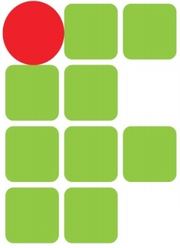
\includegraphics[width=0.10\textwidth]{Figuras/Logo_IFMA.png}
        \end{figure}
        
        {\fontseries{b}\selectfont\MakeTextUppercase{INSTITUTO FEDERAL DE EDUCAÇÃO, CIÊNCIA E TECNOLOGIA DO MARANHÃO (IFMA) - CAMPUS SÃO LUÍS MONTE CASTELO}}
		
		{\fontseries{b}\selectfont\MakeTextUppercase{
            DIRETORIA DE ENSINO SUPERIOR - DESU\\
            DEPARTAMENTO DE ELETROELETRÔNICA - DEE\\
            ENGENHARIA ELÉTRICA INDUSTRIAL}
        }
		
		\vspace{1.75cm}        {\fontseries{b}\selectfont\MakeTextUppercase{\normalsize\imprimirautor}}\\

		
		\vspace{2cm}  
		\begin{center}
            {\fontseries{b}\selectfont\MakeTextUppercase{\imprimirtitulo}}
		\end{center}
		\vfill
		
		\vfill
		
		{\fontseries{b}\selectfont\MakeTextUppercase{\imprimirlocal}}\\
%%		\par
		{\fontseries{b}\selectfont\MakeTextUppercase\imprimirdata}
	%	\vspace*{0.1cm}
	\end{capa}
}

\imprimircapa
\include{PreTextuais/FolhadeRosto}
% Caso não utilize a Ficha Catalográfica entre na folha de rosto e retire o * de dentro do arquivo FolhadeRosto
\include{PreTextuais/FichaCatalografica}
%\include{PreTextuais/Errata}

% ---
% Inserir folha de aprovação
% ---

% Isto é um exemplo de Folha de aprovação, elemento obrigatório da NBR
% 14724/2011 (seção 4.2.1.3). Você pode utilizar este modelo até a aprovação
% do trabalho. Após isso, substitua todo o conteúdo deste arquivo por uma
% imagem da página assinada pela banca com o comando abaixo:
%
% \includepdf{folhadeaprovacao_final.pdf}
%
\begin{folhadeaprovacao}

    \begin{center}
        {\fontseries{b}\selectfont\MakeTextUppercase{\normalsize\imprimirautor}}
    \end{center}
    
    \vfill
    
    \begin{center}
        {\fontseries{b}\selectfont\MakeTextUppercase{\imprimirtitulo}}
    \end{center}
    
    \vfill
    
    \abntex@ifnotempty{\imprimirpreambulo}{%
        \hspace{.45\textwidth}
        \begin{minipage}{.5\textwidth}
            \SingleSpacing
            \imprimirpreambulo\par
            \vspace*{4pt}
            {\imprimirorientadorRotulo~\imprimirorientador\par}
            \abntex@ifnotempty{\imprimircoorientador}{%
                {\imprimircoorientadorRotulo~\imprimircoorientador}%
            }%
        \end{minipage}%
    }
    
    \vfill

    \vspace*{1cm}

    % Aprovada em: \shortstack{20 \\ \underline{\hspace{1cm}}} / \shortstack{03 \\ \underline{\hspace{1cm}}} / \shortstack{2026 \\ \underline{\hspace{1.5cm}}}.    
    % Conceito obtido: \shortstack{10 \\ \underline{\hspace{1.5cm}}}

    \noindent % Garante que não haja recuo de parágrafo no início da linha
    Data de Aprovação: \shortstack{20 \\ \underline{\hspace{1cm}}} / \shortstack{03 \\ \underline{\hspace{1cm}}} / \shortstack{2026 \\ \underline{\hspace{1.5cm}}}.
    \hfill 
    Nota: \shortstack{10 \\ \underline{\hspace{1.5cm}}}.
    
    \vspace*{0.5cm}

    \begin{center}
        {\fontseries{b}\selectfont BANCA EXAMINADORA:}
    \end{center}
    
    \vspace*{1cm}
    
    \begin{center}
        \underline{\hspace{12cm}} \\
        \textbf{Prof. Dr. Almir Souza e Silva Neto} (Orientador) \\
        Instituto Federal de Educação, Ciência e Tecnologia do Maranhão (IFMA)
        
        \vspace*{1cm}
        
        \underline{\hspace{12cm}} \\
        \textbf{Prof. Me. Francisco dos Santos Viana} (Coorientador) \\
        Instituto Federal de Educação, Ciência e Tecnologia do Maranhão (IFMA)
        
        \vspace*{1cm}
        
        \underline{\hspace{12cm}} \\
        \textbf{Prof. Dr. Ronaldo Ribeiro Correa} (Examinador 1) \\
        Instituto Federal de Educação, Ciência e Tecnologia do Maranhão (IFMA)
        
        \vspace*{1cm}
        
        \underline{\hspace{12cm}} \\
        \textbf{Prof. Esp. Airton Augusto dos Anjos Costa} (Examinador 2)\\
        Instituto Federal de Educação, Ciência e Tecnologia do Maranhão (IFMA)
    \end{center}
    
    % \vspace*{\fill}
    
    % \begin{center}
    %     \imprimirlocal, 20 de março de 2026
    % \end{center}

    
\end{folhadeaprovacao}


%\textbf{	{Orientador: \vspace{-16pt} }
%	\assinatura{\textbf{Prof. \imprimirorientador , Dr.} \\ Univ. XXX} 
%	{Coorientador: \vspace{-16pt}}   
%	\assinatura{\textbf{Prof. \imprimircoorientador , Dr.} \\ Univ. XXX}
%	
%	{Membros: \vspace{-16pt} } 
%	
%	% --- Exemplo de assinaturas em sequência ---       
%	\setlength{\ABNTEXsignwidth}{8.5cm}
%	
%	\assinatura{\textbf{Prof. Professor, Dr.} \\ Univ. XXX}
%	\assinatura{\textbf{Prof. Professor, Dr.} \\ Univ. XXX}
%	\assinatura{\textbf{Prof. Professor, Dr.} \\ Univ. XXX}
%	
%	% --- Exemplo de assinaturas lado a lado ---
%	\setlength{\ABNTEXsignwidth}{7.5cm}
	%
	%    \noindent\hfill\assinatura*{\textbf{Prof. Professor, Dr.} \\ Univ. XXX}%
	%    \hfill%
	%    \assinatura*{\textbf{Prof. Professor, Dr.} \\ Univ. XXX}%
	%    \hfill
	%    
	%    \noindent\hfill\assinatura*{\textbf{Prof. Professor, Dr.} \\ Univ. XXX}%
	%    \hfill%
	%    \assinatura*{\textbf{Prof. Professor, Dr.} \\ Univ. XXX}%
	%    \hfill}
% ---
% Dedicatória
% ---
\begin{dedicatoria}
    \vspace*{\fill}
    {%
        \noindent\hspace{.5\textwidth}
        \begin{minipage}{.5\textwidth}
            \begin{flushright}
                Dedico este trabalho a Deus e à minha família.
            \end{flushright}
        \end{minipage}%
    }
    \vspace*{3cm}
\end{dedicatoria}
% ---
% ---
% Agradecimentos
% ---
\begin{agradecimentos}

A Deus, por ter me concedido tudo o que tenho e sou, pelas bênçãos, sabedoria, capacidades intelectuais, e por sempre colocar pessoas incríveis ao longo do caminho e ao meu lado.

À minha família, meus pais João Batista e Cristiane da Mercês e irmã Chrisley Batista, que sempre estiveram ao meu lado, apoiando com recursos, orações, motivação e ânimo em meio às dificuldades ao longo de toda a minha trajetória pessoal e profissional. Não teria conseguido sem a presença deles. Em especial, à minha falecida e eterna avozinha Ângela Francisca, por nunca desistir de lutar para dar uma vida melhor à família e por ser um exemplo de superação e dedicação em minha vida.

Ao meu orientador, professor Almir Souza, por ter aceitado conduzir este trabalho e pela dedicação em meio ao seu escasso tempo e correria do dia a dia.

Ao meu coorientador, professor Francisco dos Santos, que foi um pai para mim na programação e quem me introduziu a esse vasto universo da IA. Seus conhecimentos tiveram grande impacto nesta jornada.

À banca examinadora, composta pelos professores Ronaldo Correa e Airton dos Anjos, pela disponibilidade e contribuições na finalização desta jornada tão importante.

Ao meu namorado David Gomesh, pelas noites em claro, por acreditar em mim e estar sempre ao meu lado, me apoiando e incentivando desde o início da graduação — ainda na época dos primeiros códigos em C, bem antes de a IA se popularizar.

Aos meus amigos da ABU, pelas orações e fortalecimento na fé ao longo dessa caminhada universitária, em especial ao meu amigo Marcos Davi, que se tornou como um irmão para mim, não apenas pelas orações, mas pelas palavras sinceras.

Aos meus companheiros do tempo de CAEEL, cujo convívio foi tão enriquecedor, e a todos que, de alguma forma, contribuíram para esta conquista, mesmo nos pequenos gestos.

\end{agradecimentos}
% ---
% Epígrafe
% ---
\begin{epigrafe}
    \vspace*{\fill}
    \begin{flushright}
        \textit{``Os teus olhos viram o meu embrião; todos os dias determinados para mim foram escritos no teu livro antes de qualquer um deles existir.''}
        
        (Salmos 139:16, NVI)
    \end{flushright}
    \vspace*{3cm}
\end{epigrafe}
% ---
% ---
% RESUMO
% ---
\setlength{\absparsep}{18pt} 

\begin{resumo}
O fator de potência é um indicador fundamental da eficiência energética em sistemas elétricos, sendo seu monitoramento contínuo essencial para evitar penalidades regulatórias e otimizar o consumo de energia. Este trabalho propõe o desenvolvimento de um sistema inteligente de monitoramento elétrico em tempo real, capaz de classificar diferentes tipos de cargas e estimar o fator de potência por meio da integração entre sensoriamento de baixo custo, comunicação baseada em Internet das Coisas (IoT) e modelos de aprendizado de máquina. O sistema foi implementado utilizando o sensor PZEM-004T para aquisição das grandezas elétricas, o microcontrolador NodeMCU ESP8266 para transmissão dos dados via protocolo MQTT e a plataforma Node-RED para processamento e visualização em tempo real. Os modelos de classificação e regressão foram desenvolvidos com base na arquitetura Multilayer Perceptron (MLP), treinados na plataforma Edge Impulse e exportados para execução em ambiente WebAssembly. Para validação experimental, foram coletadas 1000 amostras em ambiente laboratorial controlado para cada uma das oito classes de carga consideradas, totalizando 8000 amostras. Os resultados obtidos demonstram a viabilidade técnica da solução proposta para classificação de cargas e estimativa do fator de potência em tempo real. O sistema desenvolvido destaca-se pelo baixo custo, escalabilidade e potencial de aplicação em cenários reais, contribuindo para o avanço de soluções de monitoramento inteligente no contexto da eficiência energética.

\textbf{Palavras-chave}: Monitoramento elétrico; Fator de potência; Classificação de cargas; Redes neurais artificiais; Internet das Coisas.

\end{resumo}


% O fator de potência é um indicador fundamental da eficiência energética em sistemas elétricos, e seu monitoramento contínuo é essencial para evitar penalidades regulatórias e otimizar o consumo de energia. Este trabalho propõe o desenvolvimento de um sistema inteligente de monitoramento elétrico em tempo real, capaz de classificar diferentes tipos de cargas e estimar o fator de potência por meio da integração entre sensoriamento de baixo custo, comunicação IoT e modelos de aprendizado de máquina. O sistema foi implementado utilizando o sensor PZEM-004T para aquisição das grandezas elétricas, o microcontrolador NodeMCU ESP8266 para transmissão dos dados via protocolo MQTT e a plataforma Node-RED para processamento e visualização em tempo real. Os modelos de classificação e regressão foram desenvolvidos com base na arquitetura Multilayer Perceptron (MLP), treinados na plataforma Edge Impulse e exportados para execução em ambiente WebAssembly. Para a validação experimental, foram coletadas 1000 amostras em ambiente laboratorial controlado para cada uma das oito classes de carga consideradas, totalizando 8000 amostras. A qualidade desses dados experimentais reflete-se nos resultados obtidos, que demonstram a viabilidade técnica da solução proposta. O sistema se destaca pelo baixo custo, escalabilidade e capacidade de melhorias para operação em cenários reais, contribuindo para o avanço de sistemas de monitoramento inteligente no contexto da eficiência energética.

% O modelo de classificação atingiu acurácia de 100\%, com valores de precisão, recall e F1-score iguais a 1,0 para todas as classes. O modelo de regressão apresentou erro quadrático médio de \(8,30 \times 10^{-6}\) e erro absoluto médio de 0,00228 no conjunto de teste, com coeficiente de variância explicada de 0,9997.

% \textbf{Palavras-chave}: Aprendizado de máquina; Edge Impulse; Classificação de cargas; Estimativa do fator de potência; Node-RED; Monitoramento em tempo real.

% ---
% Abstract
% ---
\begin{resumo}[Abstract]
 \begin{otherlanguage*}{english}
   The power factor is a fundamental indicator of energy efficiency in electrical systems, and its continuous monitoring is essential to avoid regulatory penalties and optimize energy consumption. This work proposes the development of an intelligent real-time electrical monitoring system capable of classifying different types of loads and estimating the power factor through the integration of low-cost sensing, Internet of Things (IoT)-based communication, and machine learning models. The system was implemented using the PZEM-004T sensor for acquiring electrical quantities, the NodeMCU ESP8266 microcontroller for data transmission via the MQTT protocol, and the Node-RED platform for real-time processing and visualization. The classification and regression models were developed based on the Multilayer Perceptron (MLP) architecture, trained on the Edge Impulse platform, and exported for execution in a WebAssembly environment. For experimental validation, 1000 samples were collected in a controlled laboratory environment for each of the eight considered load classes, totaling 8000 samples. The obtained results demonstrate the technical feasibility of the proposed solution for real-time load classification and power factor estimation. The developed system stands out for its low cost, scalability, and potential for application in real-world scenarios, contributing to the advancement of intelligent monitoring solutions in the context of energy efficiency.

   \textbf{Keywords}: Electrical monitoring; Power factor; Load classification; Artificial neural networks; Internet of Things.
 \end{otherlanguage*}
\end{resumo}
% ---
% Inserir lista de ilustrações
\pdfbookmark[0]{\listfigurename}{lof}
\listoffigures*
\cleardoublepage

% ---
% Inserir lista de quadros
\pdfbookmark[0]{\listofquadrosname}{loq}
% \listofquadros*
\cleardoublepage

% ---
% Inserir lista de tabelas
\pdfbookmark[0]{\listtablename}{lot}
\listoftables*
\cleardoublepage

% ---
% Lista de abreviaturas e siglas
\begin{siglas}
    \item[ANEEL]   Agência Nacional de Energia Elétrica
    \item[BLE]     Bluetooth de Baixa Energia (do inglês, \textit{Bluetooth Low Energy})
    \item[CSV]     Valores Separados por Vírgula (do inglês, \textit{Comma-Separated Values})
    \item[FP]      Fator de Potência
    \item[FPU]     Unidade de Ponto Flutuante (do inglês, \textit{Floating Point Unit})
    \item[IA]      Inteligência Artificial
    \item[IoT]     Internet das Coisas (do inglês, \textit{Internet of Things})
    \item[MAE]     Erro Absoluto Médio (do inglês, \textit{Mean Absolute Error})
    \item[ML]      Aprendizado de Máquina (do inglês, \textit{Machine Learning})
    \item[MLP]     Perceptron de Múltiplas Camadas (do inglês, \textit{Multilayer Perceptron})
    \item[MQTT]    Transporte de Telemetria por Enfileiramento de Mensagens (do inglês, \textit{Message Queuing Telemetry Transport})
    \item[MSE]     Erro Quadrático Médio (do inglês, \textit{Mean Squared Error})
    \item[RNA]     Redes Neurais Artificiais
    \item[RX]      Recepção do sinal
    \item[TTL]     \textit{Transistor-Transistor Logic} 
    \item[TX]      Transmissão do sinal
    \item[UART]    Receptor-Transmissor Assíncrono Universal (do inglês, \textit{Universal Asynchronous Receiver-Transmitter})
\end{siglas}

% ---
% Lista de símbolos
\begin{comment}
\begin{simbolos}
  \item[t] Tempo discreto incremental
  \item[T] Tempo finito 
  \item[$S$] Conjunto de todos os estados existentes no ambiente
  \item[$s_t$] Estado do agente no ambiente no instante t
  \item[$H$] Conjunto das observações do agente - história
%  \item[$S_t^a$]Estado do agente perante a história
  \item[$S_t^e$] Estado do ambiente
   \item[$O$] Observações sobre ambiente
  \item[$P(S_{t+1}|S_t)$] Probabilidade de transição de $S_t$ para o estado $S_{t+1}$
  \item[$k$] Elemento incremental discreto
  \item[$R_t$] Função retorno ou recompensa no tempo final $t$
  \item[$^\gamma$] Parâmetro de taxa de desconto
  \item[$A(S)$] Conjunto de ações disponíveis nos estados $S$
  \item[$a$] Uma ação tomada em determinado estado $s$
  \item[$\pi$] Uma política (regra de tomada de decisão)
  \item[$\pi^*$] Uma política ótima
  \item[$V$] Valor estado
  \item[$Q$] Valor ações
   \item[$e$]  Traço de Elegibilidade 
  
\end{simbolos}
\end{comment}
% ---

% ---
% inserir o Sumario

% Norma Relatorio de Pesquisa:
% A palavra SUMÁRIO deve estar centralizada, em letras maiúsculas e em negrito. O
% sumário é formado pelo indicativo ou número da seção, o título da seção e a página
% correspondente ao texto. Os indicativos ou números de seções que acompanham seus
% respectivos títulos devem ser apresentados alinhados à margem esquerda da página. Os
% elementos pré-textuais (capa, folha de rosto, resumo e sumário) não devem constar no
% sumário. A contagem das páginas se inicia depois da capa, a partir da folha de rosto. Mas a
% impressão dos números começa na primeira página dos elementos textuais – INTRODUÇÃO).

% ---
\pdfbookmark[0]{\contentsname}{toc}
\tableofcontents*
\cleardoublepage
% ---


% ---------------------------------------------------------------
% ELEMENTOS TEXTUAIS
% ---------------------------------------------------------------
\textual

%\pagestyle{PagNumReduzida}						% Comando para cabeçalho somente com numeração de página 10pt, quando comentado libera o pacote \usepackage{fancyhdr}
\aliaspagestyle{chapter}{PagNumReduzida}% Deixar numeração da primeira página com tamanho igual ao resto da numeração
% ref.: https://groups.google.com/g/abntex2/c/CP7g8ZMgi-c/m/KjfEnn5b9a4J

 %--------------------------------
% Introdução 
%-------------------------------
\chapter{Introdução} \label{Introdução}
A eficiência energética tem se tornado um aspecto cada vez mais relevante no contexto das unidades consumidoras, tanto do ponto de vista econômico quanto operacional. Nesse cenário, o fator de potência (FP) destaca-se como um importante indicador da qualidade e do aproveitamento da energia elétrica, uma vez que expressa a relação entre a potência ativa, efetivamente convertida em trabalho útil, e a potência aparente fornecida pela rede elétrica. Sendo assim, um baixo fator de potência está diretamente associado à presença excessiva de cargas reativas, como motores elétricos, transformadores e outros equipamentos indutivos, resultando em aquecimento dos condutores, sobrecarga de equipamentos e aumento de perdas elétricas, reduzindo a eficiência energética geral do sistema e prejudicando o desempenho dos dispositivos de utilização \cite{TecnicasDeMelhoriasFP}.

No Brasil, valores de fator de potência abaixo de 0,92 em unidades consumidoras podem acarretar penalidades aplicadas pelas concessionárias de energia, elevando os custos operacionais das unidades e, em certos casos, levando à exigência formal de correção do FP conforme regulamentações da Agência Nacional de Energia Elétrica (ANEEL, resolução nº 456/2010). Essas penalidades têm o objetivo de incentivar o uso mais eficiente da rede elétrica, uma vez que um FP reduzido implica maior demanda por potência aparente e, consequentemente, maior utilização da capacidade da rede, que poderia ser destinada a outras cargas \cite{Baixofatordepotencia}.

Para detectar e, eventualmente, corrigir valores baixos de fator de potência, torna-se necessário dispor de sistemas capazes de registrar com precisão os principais parâmetros elétricos, como tensão, corrente, potência ativa e reativa, e o próprio FP, em intervalos de tempo reduzidos. Dispositivos como os medidores inteligentes (\textit{smart meters}) fazem parte das tecnologias emergentes que permitem a aquisição automatizada e contínua desses dados, suportando aplicações de controle e otimização de redes elétricas modernas \cite{MedidoresInteligentes}. Esses dispositivos possibilitam leituras em tempo quase real, permitindo análises mais detalhadas do comportamento energético de uma instalação.

Entretanto, mesmo com a disponibilidade de medidores inteligentes, o monitoramento do fator de potência ainda é, em muitas aplicações, realizado de forma predominantemente reativa, limitando-se ao registro de valores após a ocorrência de variações significativas. Essa limitação torna-se ainda mais crítica no contexto das \textit{smart grids}, nas quais grandes volumes de dados elétricos estão disponíveis, mas ainda existem lacunas quanto ao uso desses dados para a análise inteligente do comportamento das cargas e para o suporte à tomada de decisões mais proativas \cite{MedidoresInteligentes}.

\newpage
Diante desse cenário, este trabalho propõe o desenvolvimento de um sistema de monitoramento elétrico baseado na integração entre sensoriamento, comunicação IoT e modelos de aprendizado de máquina, capaz de identificar o comportamento de diferentes tipos de carga e estimar o fator de potência em tempo real.

% --------------------------------------
% Motivação e Justificativa
% --------------------------------------
\section{Motivação e justificativa}
Com o avanço da inteligência artificial e o crescente consumo de energia elétrica, torna-se cada vez mais necessário o uso de sistemas capazes de caracterizar e monitorar cargas, permitindo estimar comportamentos e subsidiar o planejamento energético. Em ambientes industriais e comerciais, a identificação precisa do perfil das cargas e o monitoramento contínuo do fator de potência são fundamentais para a eficiência operacional, a segurança das instalações e a prevenção de penalidades regulatórias.

Nesse contexto, as redes neurais artificiais têm se tornado alternativas promissoras, capazes de extrair padrões relevantes e identificar comportamentos associados ao perfil das cargas elétricas. A partir da análise de grandezas elétricas, esses modelos podem auxiliar na caracterização das cargas conectadas ao sistema, bem como na estimativa de variáveis relevantes para a avaliação da qualidade da energia. Paralelamente, o avanço das tecnologias de Internet das Coisas (IoT) tem possibilitado a coleta e transmissão de dados elétricos em tempo real por meio de dispositivos de baixo custo, permitindo a construção de sistemas de monitoramento inteligentes e distribuídos.

Apesar dos avanços em medição elétrica e IoT, ainda são escassas as soluções que integram aquisição de dados, aprendizado de máquina e monitoramento em tempo real, especialmente em plataformas de baixo custo e fácil replicação. Nesse contexto, justifica-se o desenvolvimento de um sistema que una essas tecnologias para oferecer monitoramento inteligente e acessível.

% --------------------------------------
% Objetivos
% --------------------------------------
\section{Objetivos}
Desenvolver um sistema inteligente de monitoramento elétrico acessível e em tempo real capaz de classificar diferentes tipos de cargas e estimar o fator de potência, integrando sensoriamento de baixo custo, comunicação IoT e modelos de aprendizado de máquina.

\subsection{Objetivos Específicos}
\begin{itemize}    
    \item Realizar a aquisição de grandezas elétricas utilizando um sensor de baixo custo;

    \item Construir uma base de dados experimental contendo diferentes configurações de cargas elétricas (resistivas, indutivas, capacitivas e mistas), obtidas por meio de medições em ambiente laboratorial;
    
    \item Realizar uma análise estatística dos dados coletados para apoiar o desenvolvimento dos modelos de aprendizado de máquina;
    
    \item Desenvolver modelos de aprendizado de máquina para classificação de cargas e estimativa do fator de potência;
    
    \item Realizar a integração da aquisição de dados e da comunicação IoT em uma plataforma acessível para processamento dos modelos;
    
    \item Realizar a integração dos modelos treinados ao sistema de processamento para inferência e validação em tempo real sob condições controladas;
    
    \item Desenvolver uma interface de monitoramento para visualização em tempo real das grandezas elétricas medidas e dos resultados obtidos pelos modelos.
\end{itemize}

%-------------
% Trabalhos Relacionados/Revisão da Literatura
%-------------
\section{Trabalhos Relacionados}
Diversos trabalhos na literatura têm investigado a aplicação de técnicas de aprendizado de máquina no contexto de sistemas elétricos, especialmente na análise de dados energéticos e na modelagem de variáveis associadas ao consumo de energia e à qualidade da energia elétrica. Essas abordagens buscam auxiliar o gerenciamento energético, a detecção de ineficiências e a tomada de decisões em sistemas de potência.

Entre os métodos utilizados, as Redes Neurais Artificiais (RNAs) destacam-se como ferramentas eficazes para a modelagem de fenômenos não lineares presentes em sistemas elétricos. \citeonline{Abelem1994} investigou o uso de RNAs na modelagem de séries temporais, demonstrando que esses modelos são capazes de capturar relações complexas entre variáveis e representar adequadamente comportamentos dinâmicos observados em diferentes tipos de dados.

Em aplicações no domínio energético, \citeonline{2BrunoMontibeller} analisaram o uso de técnicas de inteligência artificial na previsão do consumo de energia elétrica em instalações, evidenciando que modelos baseados em redes neurais apresentam desempenho satisfatório mesmo em ambientes com comportamento dinâmico e não linear. De forma complementar, o estudo apresentado em \citeonline{5FerreiraMantiniano} avalia o desempenho de redes neurais do tipo \textit{Multilayer Perceptron} (MLP) na modelagem de variáveis energéticas, destacando que essa arquitetura, quando adequadamente configurada, pode apresentar bons resultados mesmo com estruturas relativamente simples.

No que se refere especificamente ao fator de potência, \citeonline{bayindir2009} propôs um sistema de correção inteligente baseado em redes neurais artificiais, demonstrando que técnicas de aprendizado de máquina podem ser utilizadas para identificar padrões de comportamento do sistema elétrico e auxiliar em estratégias de compensação do fator de potência. Estudos mais recentes também exploram a aplicação de algoritmos de aprendizado de máquina na análise e estimativa dessa variável. Em \citeonline{gamezmedina2022}, por exemplo, é apresentada uma abordagem para previsão do fator de potência em sistemas trifásicos utilizando dados reais de medições elétricas, obtendo bons níveis de acurácia. De forma complementar, \citeonline{faccin2024} realiza uma análise comparativa entre diferentes algoritmos de aprendizado de máquina aplicados a variáveis energéticas, evidenciando a competitividade de modelos baseados em MLP em termos de desempenho e simplicidade computacional.

A partir da análise dos trabalhos apresentados, observa-se que técnicas de aprendizado de máquina têm sido amplamente utilizadas para análise e modelagem de variáveis elétricas em sistemas de energia. Entretanto, grande parte dos estudos concentra-se na previsão de consumo ou em estratégias específicas de correção do fator de potência, sem explorar, de forma integrada, a aquisição de grandezas elétricas em tempo real, o monitoramento contínuo, a identificação do comportamento das cargas e a estimativa de variáveis relacionadas à qualidade da energia.

% --------------------------------------
% Contribuições do Trabalho
% --------------------------------------
\section{Contribuições do Trabalho}
Este trabalho busca contribuir para a melhoria da eficiência energética e para a consolidação da aplicação prática de técnicas de aprendizado de máquina em tempo real, disponibilizando uma solução replicável que une sensoriamento, IoT e aprendizado de máquina para monitoramento inteligente de cargas e estimativa do fator de potência.

% --------------------------------------
% Estrutura do trabalho
% --------------------------------------
\section{Estrutura do Trabalho}
Subsequente a este capítulo, o Capítulo \ref{Fundamentação Teórica} apresenta a fundamentação teórica necessária para a compreensão da pesquisa, abordando conceitos relacionados ao fator de potência, análise de dados energéticos, redes neurais artificiais e técnicas de aprendizado de máquina. O Capítulo \ref{Metodologia} descreve a metodologia proposta, incluindo a definição das variáveis do modelo, a aquisição experimental das medições elétricas e o processo de modelagem e treinamento dos algoritmos de aprendizado de máquina. O Capítulo \ref{Resultados e Discussão} apresenta os resultados obtidos, contemplando a análise da dispersão da base de dados experimental utilizada, a avaliação do desempenho dos modelos desenvolvidos e a validação experimental do sistema proposto. Por fim, o Capítulo \ref{Conclusão} apresenta as conclusões do trabalho, destacando as principais contribuições da pesquisa e as perspectivas para trabalhos futuros.

    % Introdução
 %--------------------------------
% Fundamentação Teórica 
%-------------------------------
\chapter{Fundamentação Teórica} \label{Fundamentação Teórica}

Este capítulo apresenta os conceitos teóricos que fundamentam o desenvolvimento deste trabalho. Inicialmente são apresentados os princípios relacionados ao fator de potência. Em seguida, são discutidos conceitos de Internet das Coisas (IoT), medição e monitoramento de grandezas elétricas. Por fim, são introduzidos os fundamentos de aprendizado de máquina e redes neurais artificiais, com ênfase na arquitetura Multilayer Perceptron (MLP), utilizada neste trabalho.

\section{Fator de Potência}
O fator de potência (FP) é um importante indicador da eficiência do uso da energia elétrica em sistemas de corrente alternada, expressando a relação entre a potência ativa, efetivamente convertida em trabalho útil, e a potência aparente fornecida pela rede elétrica \cite{Stevenson1994, Glover2012}. Dessa forma, o FP permite avaliar o grau de aproveitamento da energia elétrica consumida por uma instalação, sendo amplamente utilizado como parâmetro técnico para análise da qualidade da energia e do desempenho energético dos sistemas elétricos.

Valores reduzidos de fator de potência indicam a presença significativa de potência reativa no sistema, o que pode resultar em diversos impactos negativos, tais como aumento das perdas elétricas, aquecimento excessivo de condutores, sobrecarga de transformadores, quedas de tensão, subutilização da capacidade instalada e redução da vida útil dos equipamentos \cite{Pansini2011, Mamede2018}. Além disso, no contexto regulatório brasileiro, unidades consumidoras que operam com fator de potência inferior a 0,92 estão sujeitas à cobrança de excedentes de energia reativa, conforme estabelecido pela Agência Nacional de Energia Elétrica (ANEEL), o que eleva os custos operacionais do consumidor.

Em sistemas elétricos de potência, a energia é caracterizada por três tipos fundamentais de potência: ativa, reativa e aparente. A potência ativa, medida em watts (W), corresponde à parcela da potência responsável pela realização de trabalho útil, como movimento mecânico, aquecimento ou iluminação. 

A potência reativa, medida em volt-ampère reativo (VAr), está diretamente associada à defasagem angular entre as formas de onda de tensão e corrente em sistemas de corrente alternada. Essa defasagem ocorre principalmente devido à presença de cargas indutivas, resultando em um consumo adicional de corrente \cite{Glover2012}. Embora não esteja diretamente associada à realização de trabalho útil, é necessária para a criação e manutenção de campos eletromagnéticos em equipamentos como motores e transformadores \cite{Stevenson1994}.

Conforme observado na Fig. \ref{fig:triangulo_potencias}, a combinação vetorial das potências ativa e reativa resulta na potência aparente, medida em volt-ampère (VA), que representa a potência total fornecida pelo sistema elétrico.

\begin{figure}[!htbp]
	\centering
	\caption{Relação entre as potências para o cálculo do fator de potência.}
	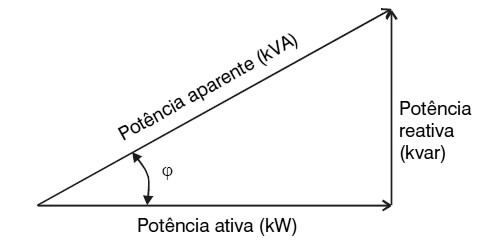
\includegraphics[width=0.6\textwidth]{Figuras/fator-de-potencia-triangulo-das-potencias.jpg}
	\fonte{Adaptado de \citeonline{engeletrica_fp}.}
	\label{fig:triangulo_potencias}
\end{figure}

Matematicamente, o fator de potência pode ser definido como a razão entre a potência ativa ($P$) e a potência aparente ($S$), conforme a Equação \ref{eq:fp}. Este indicador varia em um intervalo de 0 a 1, e quanto maior for a parcela de potência ativa em relação à potência aparente, mais elevado será o fator de potência, indicando maior eficiência energética do sistema.

\begin{equation}
    FP = \cos(\varphi) = \frac{P}{S} \quad \text{ou} \quad \frac{P}{\sqrt{P^{2} + Q^{2}}}
    \label{eq:fp}
\end{equation}

onde $P$ representa a potência ativa, $Q$ a potência reativa, $S$ a potência aparente e $\varphi$ o ângulo de defasagem entre tensão e corrente.


Assim, sistemas operando com fator de potência elevado apresentam menor circulação de corrente para uma mesma demanda de potência ativa, reduzindo perdas elétricas e melhorando o desempenho global da instalação. Por esse motivo, o monitoramento e a correção do fator de potência são práticas fundamentais para a eficiência energética, segurança operacional e conformidade regulatória em unidades consumidoras.

%------------------------------------------------------------------
%------------------------------------------------------------------
\section{Medição e Monitoramento}
A medição e o monitoramento de grandezas elétricas constituem etapas fundamentais para a análise da eficiência energética e da qualidade da energia elétrica em unidades consumidoras. Tradicionalmente, o acompanhamento elétrico em instalações de baixa e média tensão é realizado por meio de instrumentos de medição convencionais ou analisadores de energia, capazes de fornecer informações pontuais ou valores médios sobre o consumo. Entretanto, com a evolução dos sistemas elétricos e o advento do conceito de Redes Elétricas Inteligentes (\textit{Smart Grids}), destacam-se os Medidores Inteligentes (\textit{Smart Meters}), que possibilitam o registro, o armazenamento e a transmissão automatizada de dados elétricos em tempo quase real \cite{MedidoresInteligentes}.

Com o avanço das tecnologias de comunicação e o surgimento do conceito de Internet das Coisas (IoT, do inglês \textit{Internet of Things}), o monitoramento do consumo elétrico passou a ocorrer de forma mais acessível e integrada. Plataformas baseadas em IoT permitem que consumidores acompanhem seus parâmetros de consumo por meio de interfaces online, recebendo notificações e alertas quando determinados limites são atingidos, o que auxilia no controle dos gastos energéticos e na tomada de decisões \cite{GerenciadorMedidorInteligente}. 

Do ponto de vista técnico, a aquisição contínua desses parâmetros mostra-se importante para compreender o comportamento dinâmico das cargas, identificar ineficiências operacionais e detectar anomalias no sistema elétrico, como picos de consumo anormais, que podem indicar falhas ou desperdício de energia \cite{Wang2018}. Entretanto, equipamentos de medição mais avançados geralmente apresentam elevado custo de aquisição e manutenção. 

Nesse contexto, o uso de sensores elétricos de baixo custo associados a plataformas de comunicação IoT tem se tornado uma alternativa viável para a implementação de sistemas de monitoramento em tempo real, possibilitando a coleta contínua de dados que podem ser posteriormente utilizados em modelos de análise e previsão.

%------------------------------------------------------------------
%------------------------------------------------------------------
\section{Internet das Coisas}

O termo Internet das Coisas (\textit{Internet of Things} – IoT) refere-se ao paradigma tecnológico no qual objetos físicos são equipados com sensores, atuadores, capacidade de processamento e comunicação em rede, permitindo que esses dispositivos coletem, transmitam e compartilhem dados por meio da Internet. Nesse contexto, dispositivos conectados passam a interagir entre si e com sistemas computacionais, possibilitando a criação de aplicações capazes de monitorar e controlar processos de forma remota e em tempo real \cite{IoT2015}.

A arquitetura de sistemas IoT geralmente envolve dispositivos de borda (como microcontroladores), protocolos de comunicação (como MQTT, HTTP e CoAP) e plataformas em nuvem ou locais para processamento e visualização dos dados \cite{Majhi2024}. Dispositivos como o ESP8266, de baixo custo e amplamente utilizado para conectividade, permitem a integração de sensores e a transmissão de dados via Wi-Fi, viabilizando aplicações de monitoramento distribuído.

A utilização de IoT tem possibilitado o desenvolvimento de sistemas inteligentes em diferentes áreas, como automação residencial, cidades inteligentes, monitoramento industrial e sistemas de energia. Em aplicações de monitoramento elétrico, dispositivos IoT podem ser utilizados para adquirir grandezas elétricas por meio de sensores e transmiti-las para plataformas de processamento e visualização de dados (como Node-RED, ThingsBoard, etc) \cite{Msane2024, ScientificReports2025}. %Dessa forma, a integração entre sensoriamento, comunicação em rede e processamento de dados permite o desenvolvimento de soluções capazes de monitorar e analisar o comportamento de sistemas elétricos em tempo real \cite{Msane2024, ScientificReports2025}.

%------------------------------------------------------------------
%------------------------------------------------------------------
\section{Aprendizado de Máquina}
O Aprendizado de Máquina (ML, do inglês \textit{Machine Learning}) é uma área da Inteligência Artificial (IA) dedicada ao desenvolvimento de métodos computacionais capazes de aprender a partir de dados, sem a necessidade de serem explicitamente programados para cada tarefa específica \cite{Samuel1959}. Esses métodos utilizam algoritmos que identificam padrões e regularidades em conjuntos de dados e os representam por meio de modelos matemáticos, os quais podem ser posteriormente utilizados para realizar inferências ou previsões sobre novos dados \cite{1deepLearningTempestade}.

De modo geral, o Aprendizado de Máquina pode ser classificado em quatro categorias principais, conforme ilustrado na Figura \ref{fig:tipos de aprendizado de maquina}: aprendizado supervisionado, no qual o modelo é treinado a partir de dados rotulados; aprendizado não supervisionado, que busca identificar estruturas ou padrões em dados não rotulados; aprendizado semi-supervisionado, que combina dados rotulados e não rotulados; e o aprendizado por reforço, baseado na interação de um agente com o ambiente por meio de recompensas e penalidades \cite{nambundo2025}.

Durante o processo de aprendizado, o modelo ajusta iterativamente seus parâmetros internos com o objetivo de minimizar erros ou maximizar métricas de desempenho associadas à tarefa em questão. Dessa forma, o sistema é capaz de aprimorar sua capacidade de generalização, ou seja, de produzir respostas adequadas mesmo diante de dados não previamente observados \cite{Sarker2021}.

\begin{figure}[!htbp]
	\centering
	\caption{Categorias do aprendizado de máquina.}
	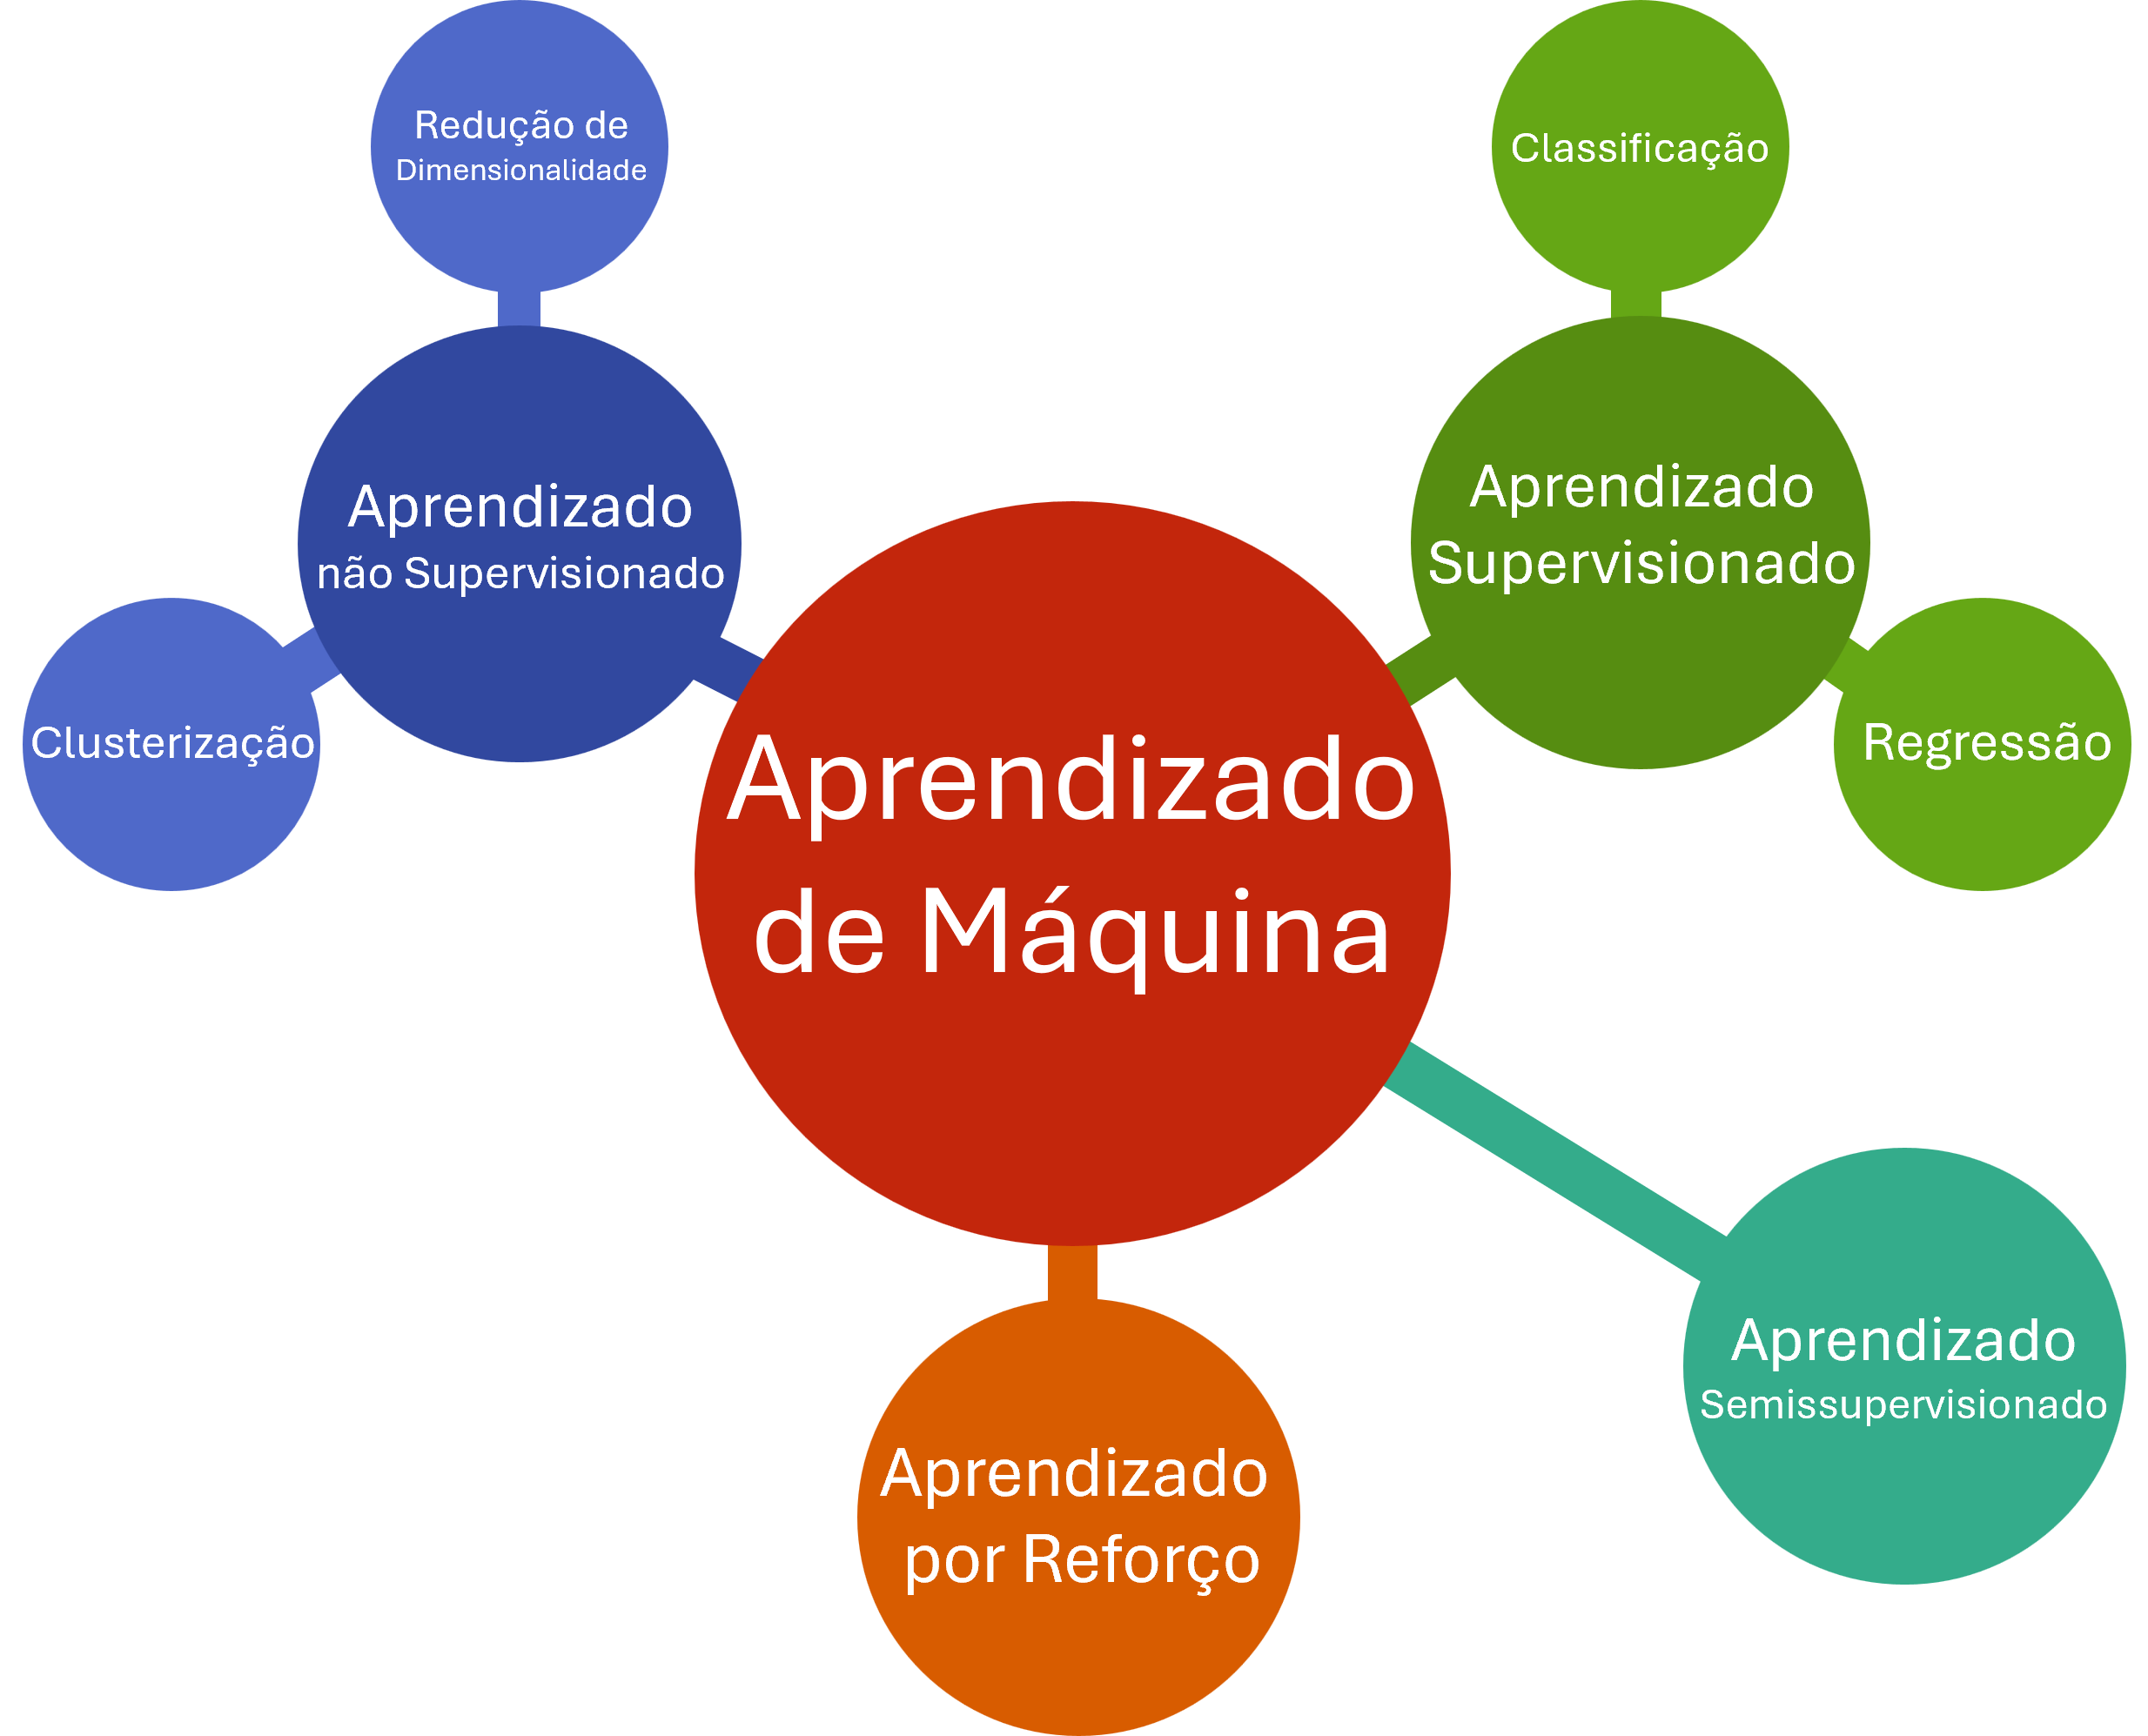
\includegraphics[width=0.83\textwidth]{Figuras/areas_ML (3).png}
	\fonte{Adaptado de \citeonline{TwipeML}.}
	\label{fig:tipos de aprendizado de maquina}
\end{figure}

Entre os diversos algoritmos desenvolvidos no contexto do aprendizado de máquina, as redes neurais artificiais têm se destacado ao longo dos anos devido à sua estrutura flexível e à capacidade de modelar relações não lineares complexas \cite{Bishop1994}. Essas características tornam as redes neurais especialmente adequadas para aplicações em problemas de classificação e regressão, abrangendo desde arquiteturas mais simples até modelos mais profundos e sofisticados \cite{Sarker2021}.

\subsection{Aprendizado de Máquina Supervisionado}
% É o termo geral utilizado para modelos nos quais os dados de treinamento incluem tanto valores de características quanto valores de rótulos conhecidos
% que são treinados a partir de um conjunto de dados rotulados, ou seja, onde os valores de entrada (características) estão associados a um valor de saída conhecido (rótulo) \cite{microsoft_classificacao}.

Conforme ilustrado na Figura \ref{fig:tipos de aprendizado de maquina}, o aprendizado de máquina supervisionado pode ser dividido em duas principais categorias:

\begin{itemize}
    \item \textbf{Classificação}: a variável de saída é qualitativa, assumindo valores discretos que representam categorias ou classes. O objetivo é aprender uma fronteira de decisão que permita atribuir cada nova observação a uma categoria específica. Quando existem apenas duas classes possíveis, o problema é denominado classificação binária, para três ou mais categorias, trata-se de classificação multiclasses \cite{codecademy_classification, microsoft_classificacao}.
    
    \item \textbf{Regressão}: a variável de saída é quantitativa, assumindo valores contínuos. O objetivo é modelar a relação entre as variáveis de entrada e um valor numérico a ser estimado. A regressão busca encontrar uma função que melhor represente a tendência dos dados, minimizando o erro entre os valores previstos e os reais \cite{ibm_regressao}.
\end{itemize}

% \begin{figure}[!htbp]
%     \centering
%     \caption{Principais categorias do aprendizado supervisionado.}
%     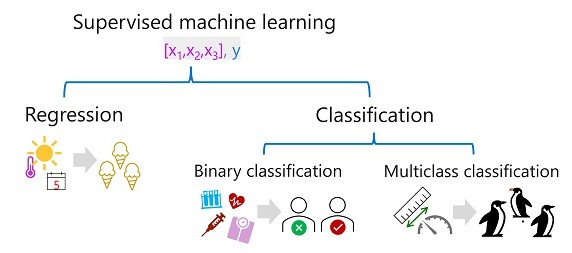
\includegraphics[scale=0.7]{Figuras/supervised-machine-learning-types.jpg}
%     \fonte{Adaptado de \citeonline{microsoft_classificacao}.}
%     \label{fig:tipos_aprendizado_supervisionado}
% \end{figure}

A Tabela \ref{tab:comparacao_class_reg} sintetiza as principais diferenças entre as duas abordagens.

\begin{table}[h]
    \centering
    \caption{Comparação entre classificação e regressão}
    \label{tab:comparacao_class_reg}
    \begin{tabular}{lcc}
    \hline
    \textbf{Característica} & \textbf{Classificação} & \textbf{Regressão} \\
    \hline
    Tipo da saída & Discreta (categórica) & Contínua (numérica) \\
    Objetivo & Atribuir a uma classe & Estimar um valor \\
    Exemplos & Tipo de carga, diagnóstico médico & Preço, temperatura, FP \\
    Métricas de avaliação & Acurácia, precisão, recall, F1-score & MSE, MAE, RMSE, R² \\
    \hline
    \end{tabular}
    \fonte{Adaptado de \citeonline{geeks_class_reg}.}
\end{table}



%------------------------------------------------------------------
%------------------------------------------------------------------
\section{Redes Neurais Artificiais}

As Redes Neurais Artificiais (RNAs) são modelos computacionais amplamente utilizados no contexto do Aprendizado de Máquina, inspirados no funcionamento do sistema nervoso biológico que adquirem conhecimento através da experiência \cite{NEGNEVITSKY2005}. Esses modelos são constituídos por um conjunto de unidades de processamento interconectadas, denominadas neurônios artificiais, cujas conexões, chamadas de sinapses, são associadas a pesos ajustáveis para transmissão das informações entre os demais neurônios. Por meio do ajuste desses pesos durante o processo de aprendizagem, as RNAs são capazes de adquirir conhecimento a partir de dados, armazenando-o de forma distribuída na rede \cite{IvanSilva2010}.

De modo geral, as RNAs apresentam características importantes, como capacidade de adaptação, generalização, aprendizado a partir de exemplos e tolerância a ruídos, o que as torna especialmente adequadas para problemas complexos envolvendo relações não lineares, como classificação, regressão e previsão de séries temporais. Em razão dessas propriedades, as redes neurais constituem uma das principais técnicas dentro do campo do Aprendizado de Máquina, o qual, por sua vez, integra o domínio mais amplo da Inteligência Artificial, conforme ilustrado na Figura \ref{fig:hierarquiaIA}.

\begin{figure}[!htbp]
	\centering
	\caption{Organização das principais áreas da Inteligência Artificial.}
	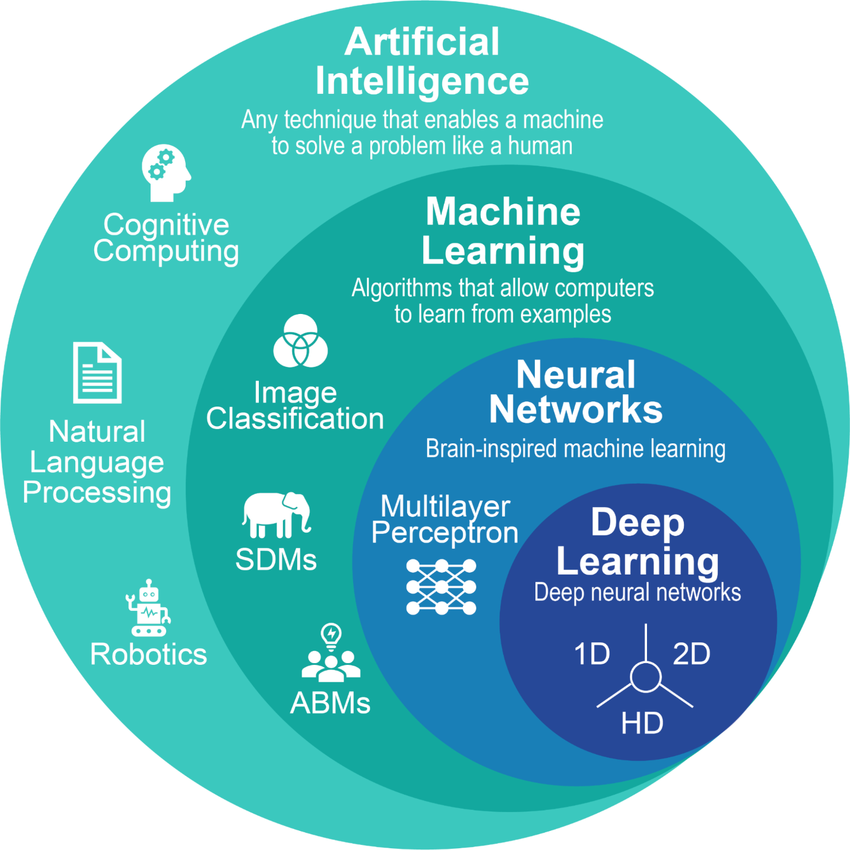
\includegraphics[width=0.47\textwidth]{Figuras/hierarquiaIA.png}
	\fonte{Adaptado de \cite{AI_Landscape_Ecology_2024}.}
	\label{fig:hierarquiaIA}
\end{figure}

% Os primeiros estudos formais sobre redes neurais artificiais remontam à década de 40, com os trabalhos de Warren S. McCulloch e Walter Pitts, que propuseram um modelo matemático simplificado do neurônio biológico e demonstraram como seu comportamento poderia ser representado artificialmente \cite{MCCULLOCH1943}. Posteriormente, em 1949, Donald Hebb introduziu o conceito de aprendizado em redes neurais por meio do ajuste das conexões sinápticas, em seu trabalho intitulado \textit{“The organization of Behavior”}, defendendo que o fortalecimento dessas conexões ocorre quando neurônios são ativados simultaneamente, princípio que ficou conhecido como regra de Hebb \cite{Passos2017}.

% Em 1958, Frank Rosenblatt apresentou o \textit{perceptron}, considerado o primeiro modelo de rede neural artificial capaz de ser treinado para a classificação de padrões por meio do ajuste iterativo dos pesos sinápticos \cite{ROSENBLATT1958}. O \textit{perceptron} pertence à classe das arquiteturas do tipo \textit{feedforward} e caracteriza-se por sua simplicidade estrutural, uma vez que é constituído por apenas uma camada com um único neurônio \cite{Vinicius2017}. Esse modelo representou um marco no desenvolvimento das RNAs ao demonstrar a viabilidade do aprendizado supervisionado em sistemas artificiais, embora apresente limitações na resolução de problemas que não são linearmente separáveis. 

Os primeiros estudos sobre redes neurais artificiais surgiram na década de 1940. Warren S. McCulloch e Walter Pitts (1943) propuseram um modelo matemático do neurônio biológico, enquanto Hebb (1949) introduziu o princípio de aprendizado por meio de ajustes das conexões sinápticas, conhecido como regra de Hebb \cite{MCCULLOCH1943, Passos2017}, defendendo que o fortalecimento dessas conexões ocorre quando neurônios são ativados simultaneamente. Em 1958, Frank Rosenblatt apresentou o \textit{perceptron}, primeiro modelo de rede neural capaz de aprendizado supervisionado por ajuste iterativo dos pesos \cite{ROSENBLATT1958}. Embora limitado a problemas linearmente separáveis, o \textit{perceptron} consolidou a viabilidades do aprendizado de máquina supervisionado \cite{Vinicius2017}.

As redes neurais artificiais podem ser classificadas de acordo com sua arquitetura e com a forma de conexão entre os neurônios. Dentre as principais categorias, destacam-se as redes do tipo \textit{feedforward}, nas quais o fluxo de informação ocorre em uma única direção, da camada de entrada até a camada de saída; as redes recorrentes, caracterizadas pela realimentação das saídas como entradas para outros neurônios, permitindo a modelagem de dependências temporais; e as redes com conexões simétricas, que considera a disposição espacial dos neurônios para o ajuste dos pesos e limiares \cite{ArquiteturasRNA}.

Independentemente da arquitetura, um neurônio artificial é composto por elementos básicos comuns, conforme ilustrado na Figura \ref{fig:representacao_neuronio_artificial}. De acordo com \cite{HAYKIN2001}, esses elementos incluem: sinais de entrada $(x_i)$, pesos sinápticos $(w_i)$, um somador para a combinação linear das entradas, um termo de bias $(b)$ e uma função de ativação $g(\cdot)$, responsável por introduzir não linearidade ao modelo. A saída resultante desse processo é o sinal $(y)$ do neurônio.


% Segundo \cite{HAYKIN2001}, os principais componentes de um neurônio artificial são:
% \begin{itemize}
%     \item Sinais de entrada $(x_i)$: representam os sinais externos que alimentam o modelo, geralmente provenientes de dados normalizados ou previamente processados;
    
%     \item Pesos sinápticos $(w_i)$: são valores ajustados durante o treinamento da rede neural, responsáveis por ponderar a influência de cada sinal de entrada no neurônio;
    
%     \item Somador $(\sum)$: responsável pelo cálculo da soma ponderada das entradas, realizando a combinação linear entre os sinais de entrada e seus respectivos pesos;
    
%     \item Bias ou viés $(b)$: parâmetro adicional que permite deslocar a função de ativação, atuando como um termo independente na soma ponderada, possibilitando maior flexibilidade ao modelo e permitindo que o neurônio seja ativado mesmo quando todas as entradas possuem valor nulo;

%     \item Potencial de ativação $(u)$: resultado da combinação linear das entradas ponderadas acrescida do termo de bias, sendo este valor o argumento da função de ativação. Quando $u \geq 0$, o neurônio tende a produzir um potencial excitatório; caso contrário, o potencial é considerado inibitório;

%     \item Função de ativação $(g(\cdot))$: aplicada ao potencial de ativação, tem como objetivo introduzir não linearidade no modelo e limitar o valor do sinal de saída, geralmente em intervalos como $(0,1)$ ou $(-1,1)$;
    
%     \item Sinal de saída $(y)$: corresponde ao valor final produzido pelo neurônio, podendo ser utilizado como entrada para outros neurônios em camadas subsequentes da rede.
% \end{itemize}

% O modelo matemático de um neurônio artificial, com seus componentes fundamentais, é ilustrado na Figura \ref{fig:representacao_neuronio_artificial}. Nessa representação, observa-se um conjunto de entradas $(x_i)$ que, ao serem multiplicadas por seus respectivos pesos $(w_i)$ e posteriormente somadas, geram um sinal interno que é então aplicado a uma função de ativação que, por sua vez, é responsável por determinar o nível de ativação do neurônio, produzindo o sinal de saída da unidade neural.

\begin{figure}[!htbp]
	\centering
	\caption{Modelo de um neurônio artificial.}
	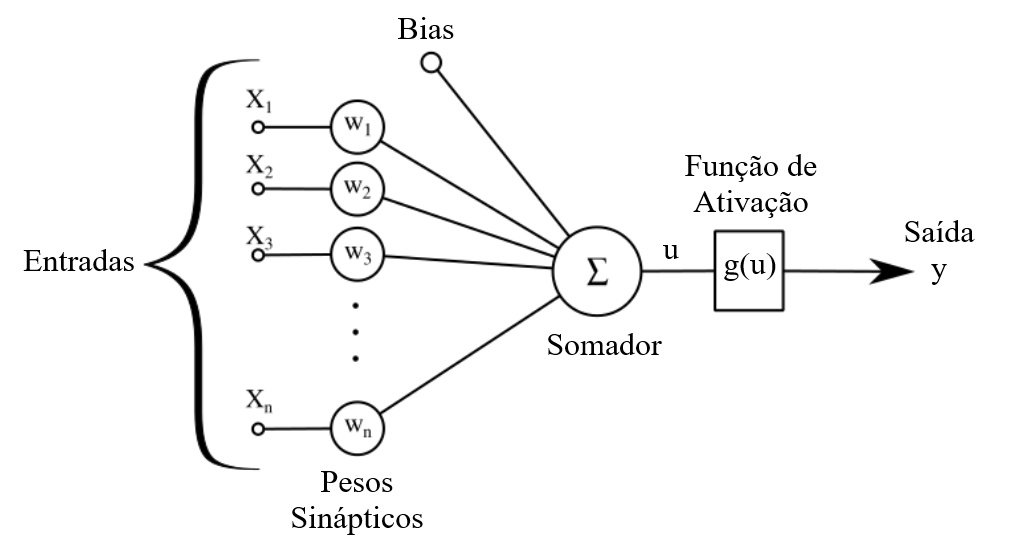
\includegraphics[width=0.8\textwidth]{Figuras/Modelo_Neuronio_Artificial.png}
	\fonte{Adaptado de \citeonline{Azevedo2016}.}
	\label{fig:representacao_neuronio_artificial}
\end{figure}

Assim, a operação matemática realizada por um neurônio artificial pode ser descrita pela Equação \ref{eq:neuronio}.

\begin{equation}
    y = g\left(\sum_{i=1}^{n} w_i x_i + b \right)
    \label{eq:neuronio}
\end{equation}

%------------------------------------------------------------------
%------------------------------------------------------------------
\subsection{Rede Neural \textit{Multilayer Perceptron (MLP)}}

A arquitetura \textit{Multilayer Perceptron (MLP)} surgiu como extensão do \textit{Perceptron} de Rosenblatt para superar sua limitação na resolução de problemas não linearmente separáveis \cite{ROSENBLATT1958, Minsky1969}. Sua principal inovação é a inclusão de uma ou mais camadas ocultas entre as camadas de entrada e saída, permitindo a representação de funções não lineares complexas, conforme ilustrado na Figura \ref{fig:representacao_mlp}.

A MLP é uma rede neural do tipo \textit{feedforward}, na qual a informação flui unidirecionalmente da entrada para a saída, sem realimentação \cite{HAYKIN2001}. Sua arquitetura básica, ilustrada na Figura \ref{fig:representacao_mlp}, é composta por três tipos de camadas:
\begin{itemize}
    \item \textbf{Camada de entrada}: responsável por receber os dados;
    \item \textbf{Camadas ocultas}: realizam transformações não lineares por meio de funções de ativação;
    \item \textbf{Camada de saída}: fornece a resposta final do modelo.
\end{itemize}

O aprendizado da MLP ocorre de forma supervisionada, ajustando os pesos sinápticos e \textit{biases} para minimizar uma função de custo, que mede o erro entre a saída estimada e o valor desejado \cite{Arquiteturadasredes}. O algoritmo mais empregado para esse fim é a retropropagação do erro (\textit{backpropagation}), que calcula os gradientes da função de custo em relação aos pesos e os ajusta por meio do gradiente descendente ou de suas variações. O erro é propagado da camada de saída para as camadas anteriores, permitindo o ajuste iterativo dos pesos sinápticos \cite{Rumelhart1986}. Outras abordagens, como métodos evolucionários, também podem ser utilizadas, dependendo das características do problema \cite{Bishop1994, HAYKIN2001}.

A MLP é amplamente utilizada em problemas de regressão e previsão de séries temporais devido à sua capacidade de aproximar funções contínuas não lineares. Essa propriedade é garantida pelo Teorema da Aproximação Universal, que estabelece que redes \textit{feedforward} com ao menos uma camada oculta e funções de ativação adequadas podem aproximar qualquer função contínua em compactos com erro arbitrariamente pequeno \cite{Cybenko1989, Hornik1989}. Ao utilizar valores passados como entrada, a MLP captura dependências temporais implícitas, sendo eficaz na modelagem de grandezas dinâmicas como demanda de energia e fator de potência \cite{Amjady2009, Andrade2015}.

Essa capacidade de modelagem não linear torna a MLP particularmente adequada para sistemas elétricos, onde variáveis como potência, corrente e fator de potência apresentam comportamento dinâmico e não linear. Além disso, sua estrutura relativamente simples, comparada a arquiteturas mais complexas, resulta em menor custo computacional durante a inferência, favorecendo sua aplicação em sistemas com recursos limitados \cite{Sarker2021}.

\begin{figure}
\caption{Rede Neural \textit{feedforward Multilayer Perceptron}.}
 \centering   
\begin{tikzpicture}[
  >={Stealth[length=3mm]},
  line/.style={->, thick},
  conn/.style={->, gray!40, thin},
  inNode/.style={
    draw=orange!80!brown, fill=orange!20,
    minimum size=6mm, rounded corners=2pt
  },
  hidNode/.style={
    circle, draw=blue!60!black, fill=blue!12,
    minimum size=11mm
  },
  outNode/.style={
    circle, draw=teal!70!black, fill=teal!18,
    minimum size=11mm
  }
]

% --- Nós de entrada ---
\node[inNode] (I1) at (0, 2.4) {};
\node[inNode] (I2) at (0, 1.2) {};
\node[inNode] (I3) at (0, -0.4) {};
\node at (0, 0.62) {\large $\vdots$};

% --- Camada oculta 1 ---
\node[hidNode] (H11) at (3, 2.4) {};
\node[hidNode] (H12) at (3, 1.2) {};
\node[hidNode] (H13) at (3, -0.4) {};
\node at (3, 0.5) {\large $\vdots$};

% --- Camada oculta 2 ---
\node[hidNode] (H21) at (6, 2.4) {};
\node[hidNode] (H22) at (6, 1.2) {};
\node[hidNode] (H23) at (6, -0.4) {};
\node at (6, 0.5) {\large $\vdots$};

% --- Nós de saída ---
\node[outNode] (O1) at (9, 1.8) {};
\node[outNode] (O2) at (9, 0.6) {};

% --- Conexões entrada -> oculta 1 ---
\foreach \i in {1,2,3}{
  \foreach \j in {1,2,3}{
    \draw[conn] (I\i) -- (H1\j);
  }
}

% --- Conexões oculta 1 -> oculta 2 ---
\foreach \i in {1,2,3}{
  \foreach \j in {1,2,3}{
    \draw[conn] (H1\i) -- (H2\j);
  }
}

% --- Conexões oculta 2 -> saída ---
\foreach \i in {1,2,3}{
  \foreach \j in {1,2}{
    \draw[conn] (H2\i) -- (O\j);
  }
}

% --- Setas de entrada ---
\draw[line, orange!80!brown] (-1.3, 2.4) -- (I1)
  node[midway, above, font=\small] {$x_1$};
\draw[line, orange!80!brown] (-1.3, 1.2) -- (I2)
  node[midway, above, font=\small] {$x_2$};
\draw[line, orange!80!brown] (-1.3, -0.4) -- (I3)
  node[midway, above, font=\small] {$x_n$};

% --- Setas de saída ---
\draw[line, teal!70!black] (O1) -- ++(1.3, 0)
  node[right, font=\small] {$\hat{y}_1$};
\draw[line, teal!70!black] (O2) -- ++(1.3, 0)
  node[right, font=\small] {$\hat{y}_2$};

% --- Chave sobre camadas ocultas ---
\draw[decorate, decoration={brace, amplitude=5pt}, blue!60!black]
  (2.2, 3.1) -- (6.8, 3.1)
  node[midway, above=5pt, font=\small\bfseries, blue!70!black]
  {Camadas ocultas};


% --- Legenda em linha ---
\node[inNode,  minimum size=3.5mm] at (1.2, -1.4) {};
\node[anchor=west, font=\scriptsize] at (1.45, -1.41) {Camada de entrada};

\node[hidNode, minimum size=4mm]   at (4.5, -1.4) {};
\node[anchor=west, font=\scriptsize] at (4.75, -1.4) {Camadas ocultas};

\node[outNode, minimum size=4mm]   at (7.5, -1.4) {};
\node[anchor=west, font=\scriptsize] at (7.75, -1.4) {Camada de saída};

\draw[gray!50, thin, rounded corners=2pt]
  (0.7, -1.8) rectangle (10.5, -1.1);


\end{tikzpicture}
\label{fig:representacao_mlp}
 \fonte{\me{2026}} 

\end{figure}

    % Fundamentação Teórica 
 %-------------
% Metodologia 

% Capítulo de materiais e métodos. Materiais é tudo aquilo que foi usado, desde recurso de hardware, notebook, bancada, motor, contator etc. Método é a descrição da ideia e sua implementação
%-------------
\chapter{Metodologia} \label{Metodologia}
O desenvolvimento deste trabalho foi estruturado em etapas complementares, abrangendo fundamentação teórica, análise exploratória de dados, aquisição experimental de medições elétricas, modelagem de algoritmos de aprendizado de máquina, implementação do sistema elétrico e validação experimental.

Inicialmente, foi realizada uma revisão bibliográfica com o objetivo de fundamentar a aplicação de redes neurais artificiais na análise de sistemas elétricos, com ênfase em modelos do tipo Multilayer Perceptron (MLP). Também foram investigadas abordagens relacionadas à execução de modelos de aprendizado de máquina próximos à fonte de dados, no contexto de aplicações de Internet das Coisas, visando possibilitar processamento e inferência em tempo real. Foram analisados trabalhos voltados à estimativa do fator de potência, à classificação de tipos de carga e à aplicação de técnicas de aprendizado de máquina em sistemas elétricos, estabelecendo a base conceitual e metodológica desta pesquisa.

Paralelamente à fundamentação teórica, foi realizada uma análise exploratória de dados utilizando a base residencial \textit{Individual Household Electric Power Consumption}, disponibilizada no repositório \textit{UC Irvine Machine Learning Repository}. Essa etapa teve como objetivo investigar o comportamento das grandezas elétricas e sua relação com o fator de potência, permitindo identificar as variáveis mais relevantes para representação do comportamento das cargas elétricas e para a estimação do fator de potência. As variáveis selecionadas foram posteriormente utilizadas como entradas nos modelos de aprendizado de máquina desenvolvidos neste trabalho.

Na etapa experimental, foi desenvolvido um sistema de aquisição de dados elétricos utilizando o sensor PZEM-004T. Na sequência, procedeu-se à modelagem das redes neurais, contemplando as etapas de treinamento e teste no ambiente Edge Impulse e validação do sistema, por meio de métricas adequadas de avaliação de desempenho. Posteriormente os modelos foram integrados ao fluxo de processamento implementado na plataforma Node-RED, responsável pela execução das inferências em tempo real. Por fim, foi implementado um painel de monitoramento para visualização e acompanhamento em tempo real das grandezas elétricas medidas e estimadas.

%------------------------------------------------------------------
%------------------------------------------------------------------
\section{Visão Geral do Sistema Proposto}

Para o desenvolvimento do sistema proposto foram seguidas as seguintes etapas:

\begin{enumerate}
    \item \textbf{Definição dos Componentes:} Nesta etapa foram selecionados os elementos de hardware necessários para a aquisição e transmissão dos dados elétricos. Foram utilizados o sensor PZEM-004T para medição das grandezas elétricas e o microcontrolador NodeMCU ESP8266 para coleta dessas leituras e transmissão dos dados para o ambiente de processamento Node-RED.
    
    \item \textbf{Definição da Arquitetura do Sistema:} Foi projetada a arquitetura funcional do sistema, estabelecendo o fluxo de dados desde a aquisição das variáveis elétricas até o processamento, implementação dos modelos e visualização dos resultados. Nesta fase foram definidos os módulos de aquisição de dados, comunicação via protocolo MQTT, inferência do modelo de aprendizado de máquina e interface de monitoramento.
    
    \item \textbf{Análise das Características das Cargas Elétricas:} Esta etapa consistiu no estudo do comportamento elétrico de diferentes tipos de cargas, considerando a relação entre tensão, corrente, potência ativa, potência reativa, potência aparente e fator de potência. Essa análise fundamentou a escolha das variáveis de entrada para os modelos.
    
    \item \textbf{Coleta de Dados em Cenários Reais:} Realizou-se a aquisição de dados elétricos em ambiente laboratorial, utilizando diferentes configurações de carga. Essa etapa teve como objetivo construir a base de dados utilizada no treinamento e validação do modelo de classificação.
    
    \item \textbf{Treinamento do Modelo de Classificação:} Envolveu o treinamento por meio da plataforma Edge Impulse e conversão dos modelos para o formato WebAssembly, possibilitando a execução no ambiente Node-RED.
    
    \item \textbf{Processamento dos Modelos:} Realização da exportação e integração dos modelos ao ambiente de processamento Node-RED, permitindo a execução da inferência em tempo real a partir dos dados medidos pelo sensor.
    
    \item \textbf{Comunicação:} Consistiu na implementação da conectividade entre o microcontrolador e o Node-RED por meio do protocolo MQTT, garantindo a atualização contínua dos dados coletados.
    
    \item \textbf{Criação do Dashboard de Monitoramento:} Desenvolvimento de uma interface gráfica utilizando a plataforma Node-RED, permitindo a visualização em tempo real das grandezas elétricas medidas, da classificação das cargas identificadas e estimativa do PF pelos modelos.
\end{enumerate}

A Figura \ref{fig:integracao_sistema} ilustra a estrutura de funcionamento do sistema proposto.

\begin{figure}[!htbp] 
    \centering 
    \caption{Estrutura funcional do sistema.} 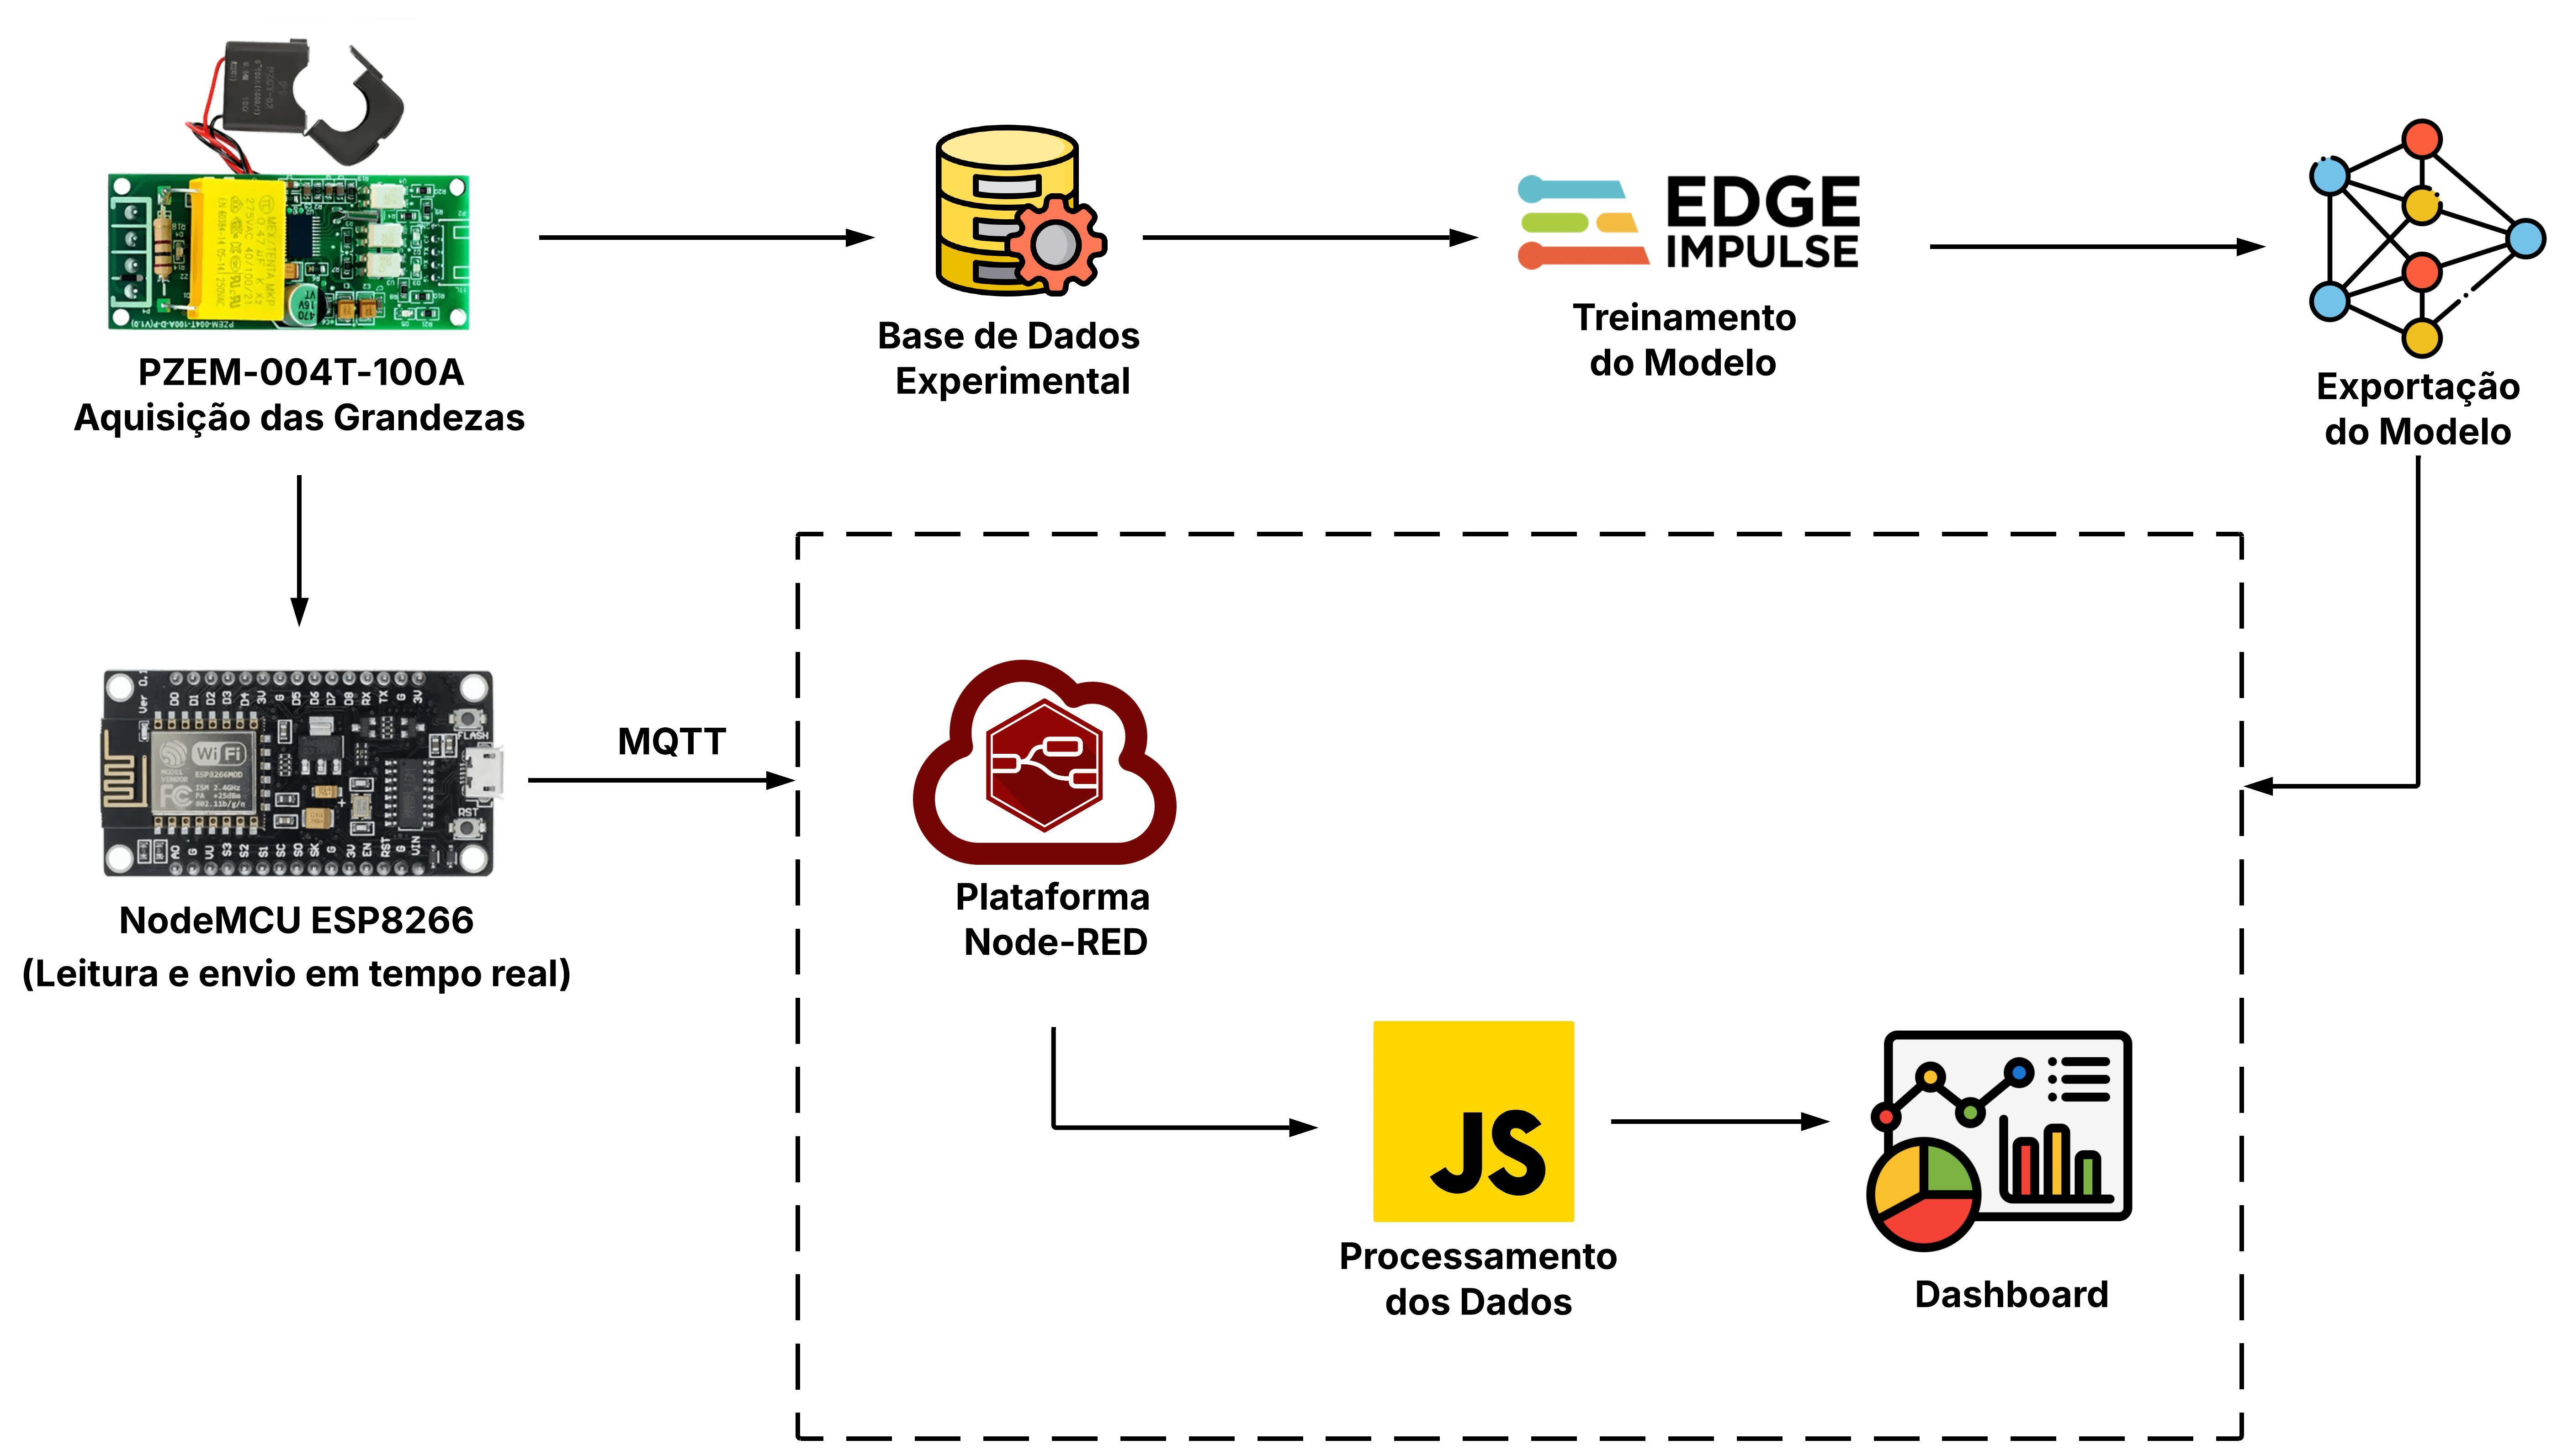
\includegraphics[width=1\textwidth]{Figuras/Integracao do sistema.jpeg} 
    \fonte{\me{2026}} 
    \label{fig:integracao_sistema} 
\end{figure}

%------------------------------------------------------------------
%------------------------------------------------------------------
\section{Materiais}
\subsection{Sensor de medição das grandezas elétrica}

Para a aquisição das grandezas elétricas necessárias ao treinamento e validação dos modelos, bem como para a visualização em tempo real dessas grandezas no painel de monitoramento, foi adotado o módulo de medição PZEM-004T-100A, mostrado na Figura \ref{fig:Medidor PZEM}. Este sensor permite a leitura de multiparâmetros elétricos em tempo real, como frequência, tensão, corrente, potência ativa, energia acumulada e fator de potência, sendo amplamente empregado em aplicações que exigem medições precisas e estáveis, como monitoramento de consumo energético.

\begin{figure}[!htbp] 
    \centering 
    \caption{Módulo PZEM-004T-100A.} 
    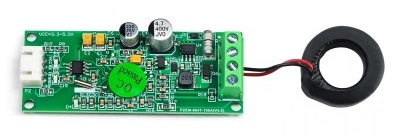
\includegraphics[width= 0.6\textwidth]{Figuras/PZEM.jpg} 
    \fonte{Extraída de \citeonline{UsinaInfo}.} 
    \label{fig:Medidor PZEM} 
\end{figure}

O módulo realiza medições em sistemas monofásicos e possui uma interface de comunicação serial TTL (\textit{Transistor-Transistor Logic} do tipo UART (\textit{Universal Asynchronous Receiver-Transmitter}), que utiliza apenas dois fios (TX e RX) para transmissão serial assíncrona, ou seja, de forma sequencial, bit a bit, sem necessidade de um sinal de clock compartilhado. Essa característica garante simplicidade e eficiência na troca de informações, facilitando a integração com microcontroladores. A Tabela \ref{tab:pzem_especificacoes} apresenta as principais especificações técnicas do sensor utilizado.

\begin{table}[!htbp]
    \centering
    \caption{Especificações técnicas do sensor PZEM-004T-100A.}
    \label{tab:pzem_especificacoes}
    \begin{tabular}{|l|c|c|}
    \hline
    \multicolumn{1}{|c|}{\textbf{Grandezas}} & \textbf{Faixa de Medição} & \textbf{Precisão (\%)} \\
    \hline
    Tensão &            80 – 260 V &        0.5 \\
    Corrente &          0 – 100 A &         0.5 \\
    Potência ativa &    0 – 23 kW &         0.5 \\
    Fator de Potência & 0,00 - 1,00 &       1.0 \\
    Energia &           0 - 9999,99 kWh &   0.5 \\
    Frequência &        45 – 65 Hz &        0.5 \\
    \hline
    \end{tabular}
    \fonte{\me{2026}}
\end{table}

Um dos grandes diferenciais deste módulo é a medição de corrente sem contato direto, feita por meio de um transformador de corrente (TC) incluso, capaz de medir até 100A AC. Diante disso, o sensor PZEM foi escolhido devido  à sua facilidade de integração, baixo custo, excelente desempenho nas medições e comunicação serial simplificada, reduzindo a complexidade do hardware.

%------------------------------------------------------------------
\subsection{NodeMCU ESP8266}
Na aquisição e transmissão dos dados elétricos foi utilizado o microcontrolador NodeMCU ESP8266, apresentado na Figura \ref{fig:nodemcu}. Este dispositivo é amplamente utilizado em aplicações de Internet das Coisas (IoT), pois integra conectividade Wi-Fi nativa, permitindo a comunicação direta com redes sem fio.

\begin{figure}[!htbp] 
    \centering
    \caption{Placa NodeMCU ESP8266.} 
    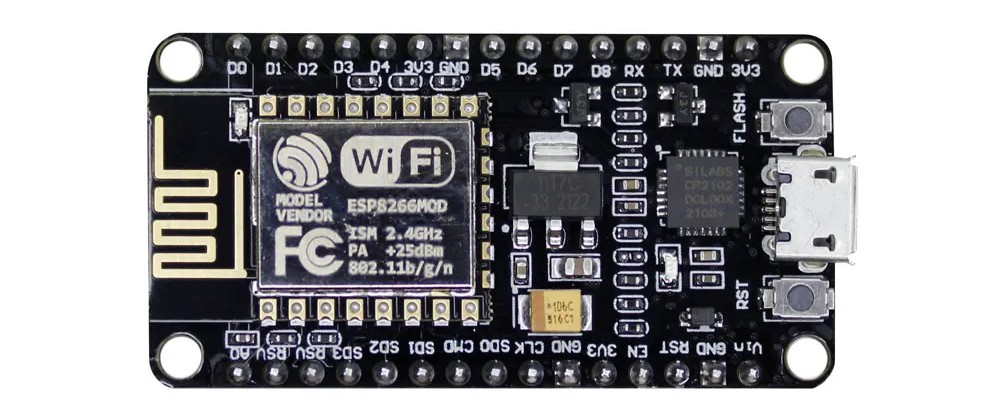
\includegraphics[width=0.6\textwidth]{Figuras/nodeMCU.jpg} 
    \fonte{Figura extraída de \citeonline{kevsrobots_esp8266}.} 
    \label{fig:nodemcu} 
\end{figure}

Conforme apresentado na Tabela \ref{tab:nodemcu_especificacoes} o NodeMCU é baseado no microcontrolador ESP8266, que possui arquitetura de 32 bits e capacidade de processamento adequada para aplicações de baixo custo. Sua principal vantagem é a integração de conectividade Wi-Fi, permitindo a transmissão dos dados coletados para plataformas de processamento e monitoramento em rede.

No sistema desenvolvido, o NodeMCU foi responsável pela leitura dos dados provenientes do sensor PZEM-004T por meio de comunicação serial e pelo envio dessas informações para o ambiente Node-RED utilizando o protocolo MQTT.

\begin{table}[!htbp]
    \centering
    \caption{Especificações técnicas do NodeMCU ESP8266}
    \label{tab:nodemcu_especificacoes}
    \begin{tabular}{|l|c|}
    \hline
    \multicolumn{1}{|c|}{\textbf{Parâmetro}} & \textbf{Especificação} \\
    \hline
    Microcontrolador & ESP8266 \\
    Arquitetura & 32 bits \\
    Frequência de operação & até 80 MHz \\
    Memória Flash & até 4 MB \\
    Conectividade & Wi-Fi 802.11 b/g/n \\
    Tensão de operação & 3,3 V \\
    GPIO & até 11 pinos de entrada/saída \\
    Interface de comunicação & UART, SPI, I2C \\
    \hline
    \end{tabular}
    \fonte{\me{2026}}
\end{table}

%------------------------------------------------------------------
\subsection{Módulo Relé}
O módulo relé, ilustrado na Figura \ref{fig:Modulo_Rele}, é um dispositivo de comutação eletromecânica que permite controlar circuitos de maior potência por meio de sinais de baixa potência provenientes do microcontrolador.

\begin{figure}[!htbp] 
    \centering
    \caption{Módulo relé utilizado para acionamento das cargas.} 
    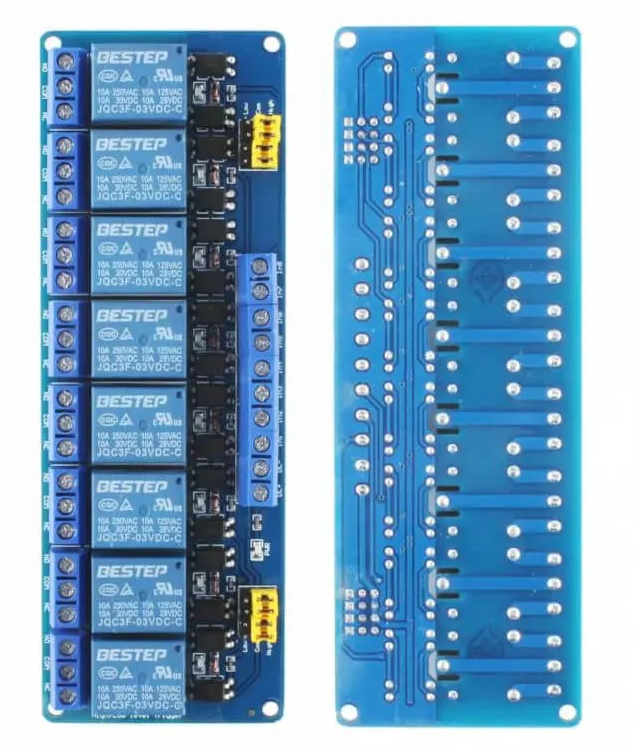
\includegraphics[width= 0.4\textwidth]{Figuras/rele8canais.png} 
    \fonte{Figura extraída de \citeonline{smartkits_rele8ch}.} 
    \label{fig:Modulo_Rele} 
\end{figure}

No sistema desenvolvido, o módulo relé foi empregado para o controle das cargas elétricas utilizadas nos experimentos, sendo acionado por sinais digitais gerados pelo microcontrolador. Quando ativado, o relé altera o estado de seus contatos internos, permitindo ou interrompendo a passagem de corrente no circuito de potência.

%------------------------------------------------------------------
\subsection{Contatores}
São dispositivos de comutação projetados para operar em circuitos de potência, sendo capazes de suportar correntes mais elevadas e maior número de ciclos de operação quando comparados a relés convencionais. Seu funcionamento baseia-se na atuação de um eletroímã que, ao ser energizado, aciona mecanicamente os contatos responsáveis pela abertura ou fechamento do circuito elétrico, conforme apresentado na Figura \ref{fig:Contactor}.

\begin{figure}[!htbp] 
    \centering
    \caption{Contator utilizado no sistema experimental.} 
    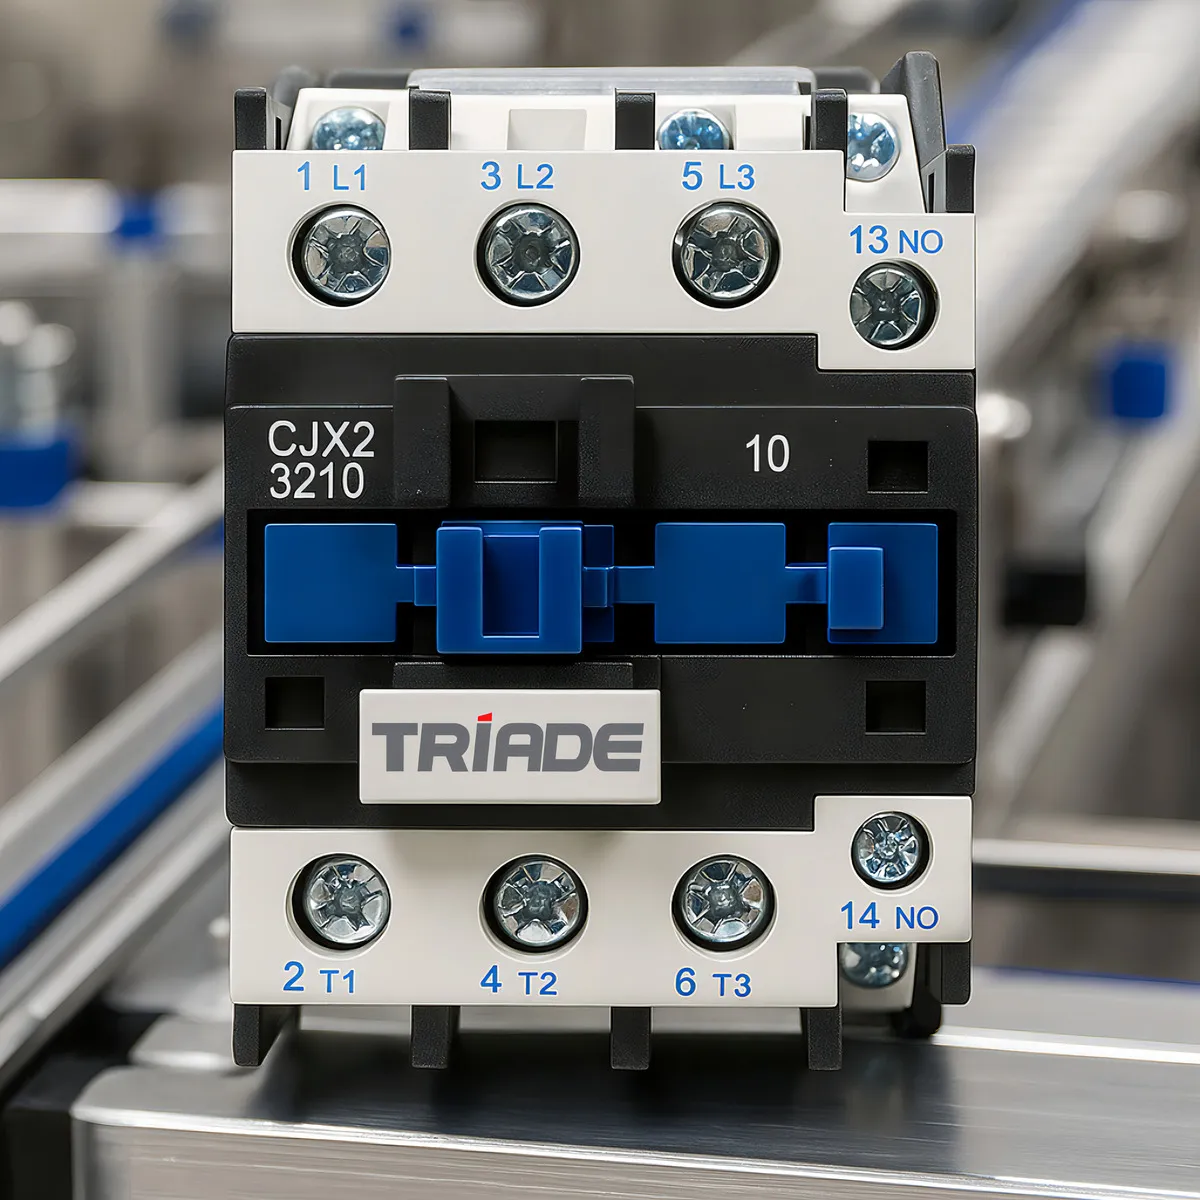
\includegraphics[width= 0.4\textwidth]{Figuras/contator.png} 
    \fonte{Figura extraída de \citeonline{ml_contator_cjx2}.} 
    \label{fig:Contactor} 
\end{figure}

Os contatores foram utilizados para o acionamento das cargas de maior potência, garantindo maior segurança elétrica e confiabilidade operacional. O controle desses dispositivos foi realizado indiretamente pelo microcontrolador por meio do módulo relé, que atua como interface de comando para a bobina do contator. Dessa forma, sinais de baixa potência provenientes do microcontrolador podem controlar cargas de maior potência de maneira segura, promovendo o isolamento entre o circuito de controle e o circuito de potência e reduzindo riscos associados à operação do sistema.

%------------------------------------------------------------------
\subsection{Integração e Ligações do Circuito}

A Figura \ref{fig:esquema_eletrico} apresenta o esquemático das conexões elétricas realizadas, detalhando a ligação entre o sensor PZEM-004T e o microcontrolador NodeMCU ESP8266, e do circuito de potência, incluindo relés, contatores e cargas. O módulo PZEM foi alimentado pelos pinos Vin e GND do NodeMCU. A comunicação entre os dispositivos ocorreu via interface serial UART, com conexão cruzada dos sinais: TX do PZEM ao RX do NodeMCU (GPIO 3) e RX do PZEM ao TX do NodeMCU (GPIO 1).

\begin{figure}[!htbp] 
    \centering
    \caption{Esquemático elétrico da aquisição de dados e controle de cargas.}
    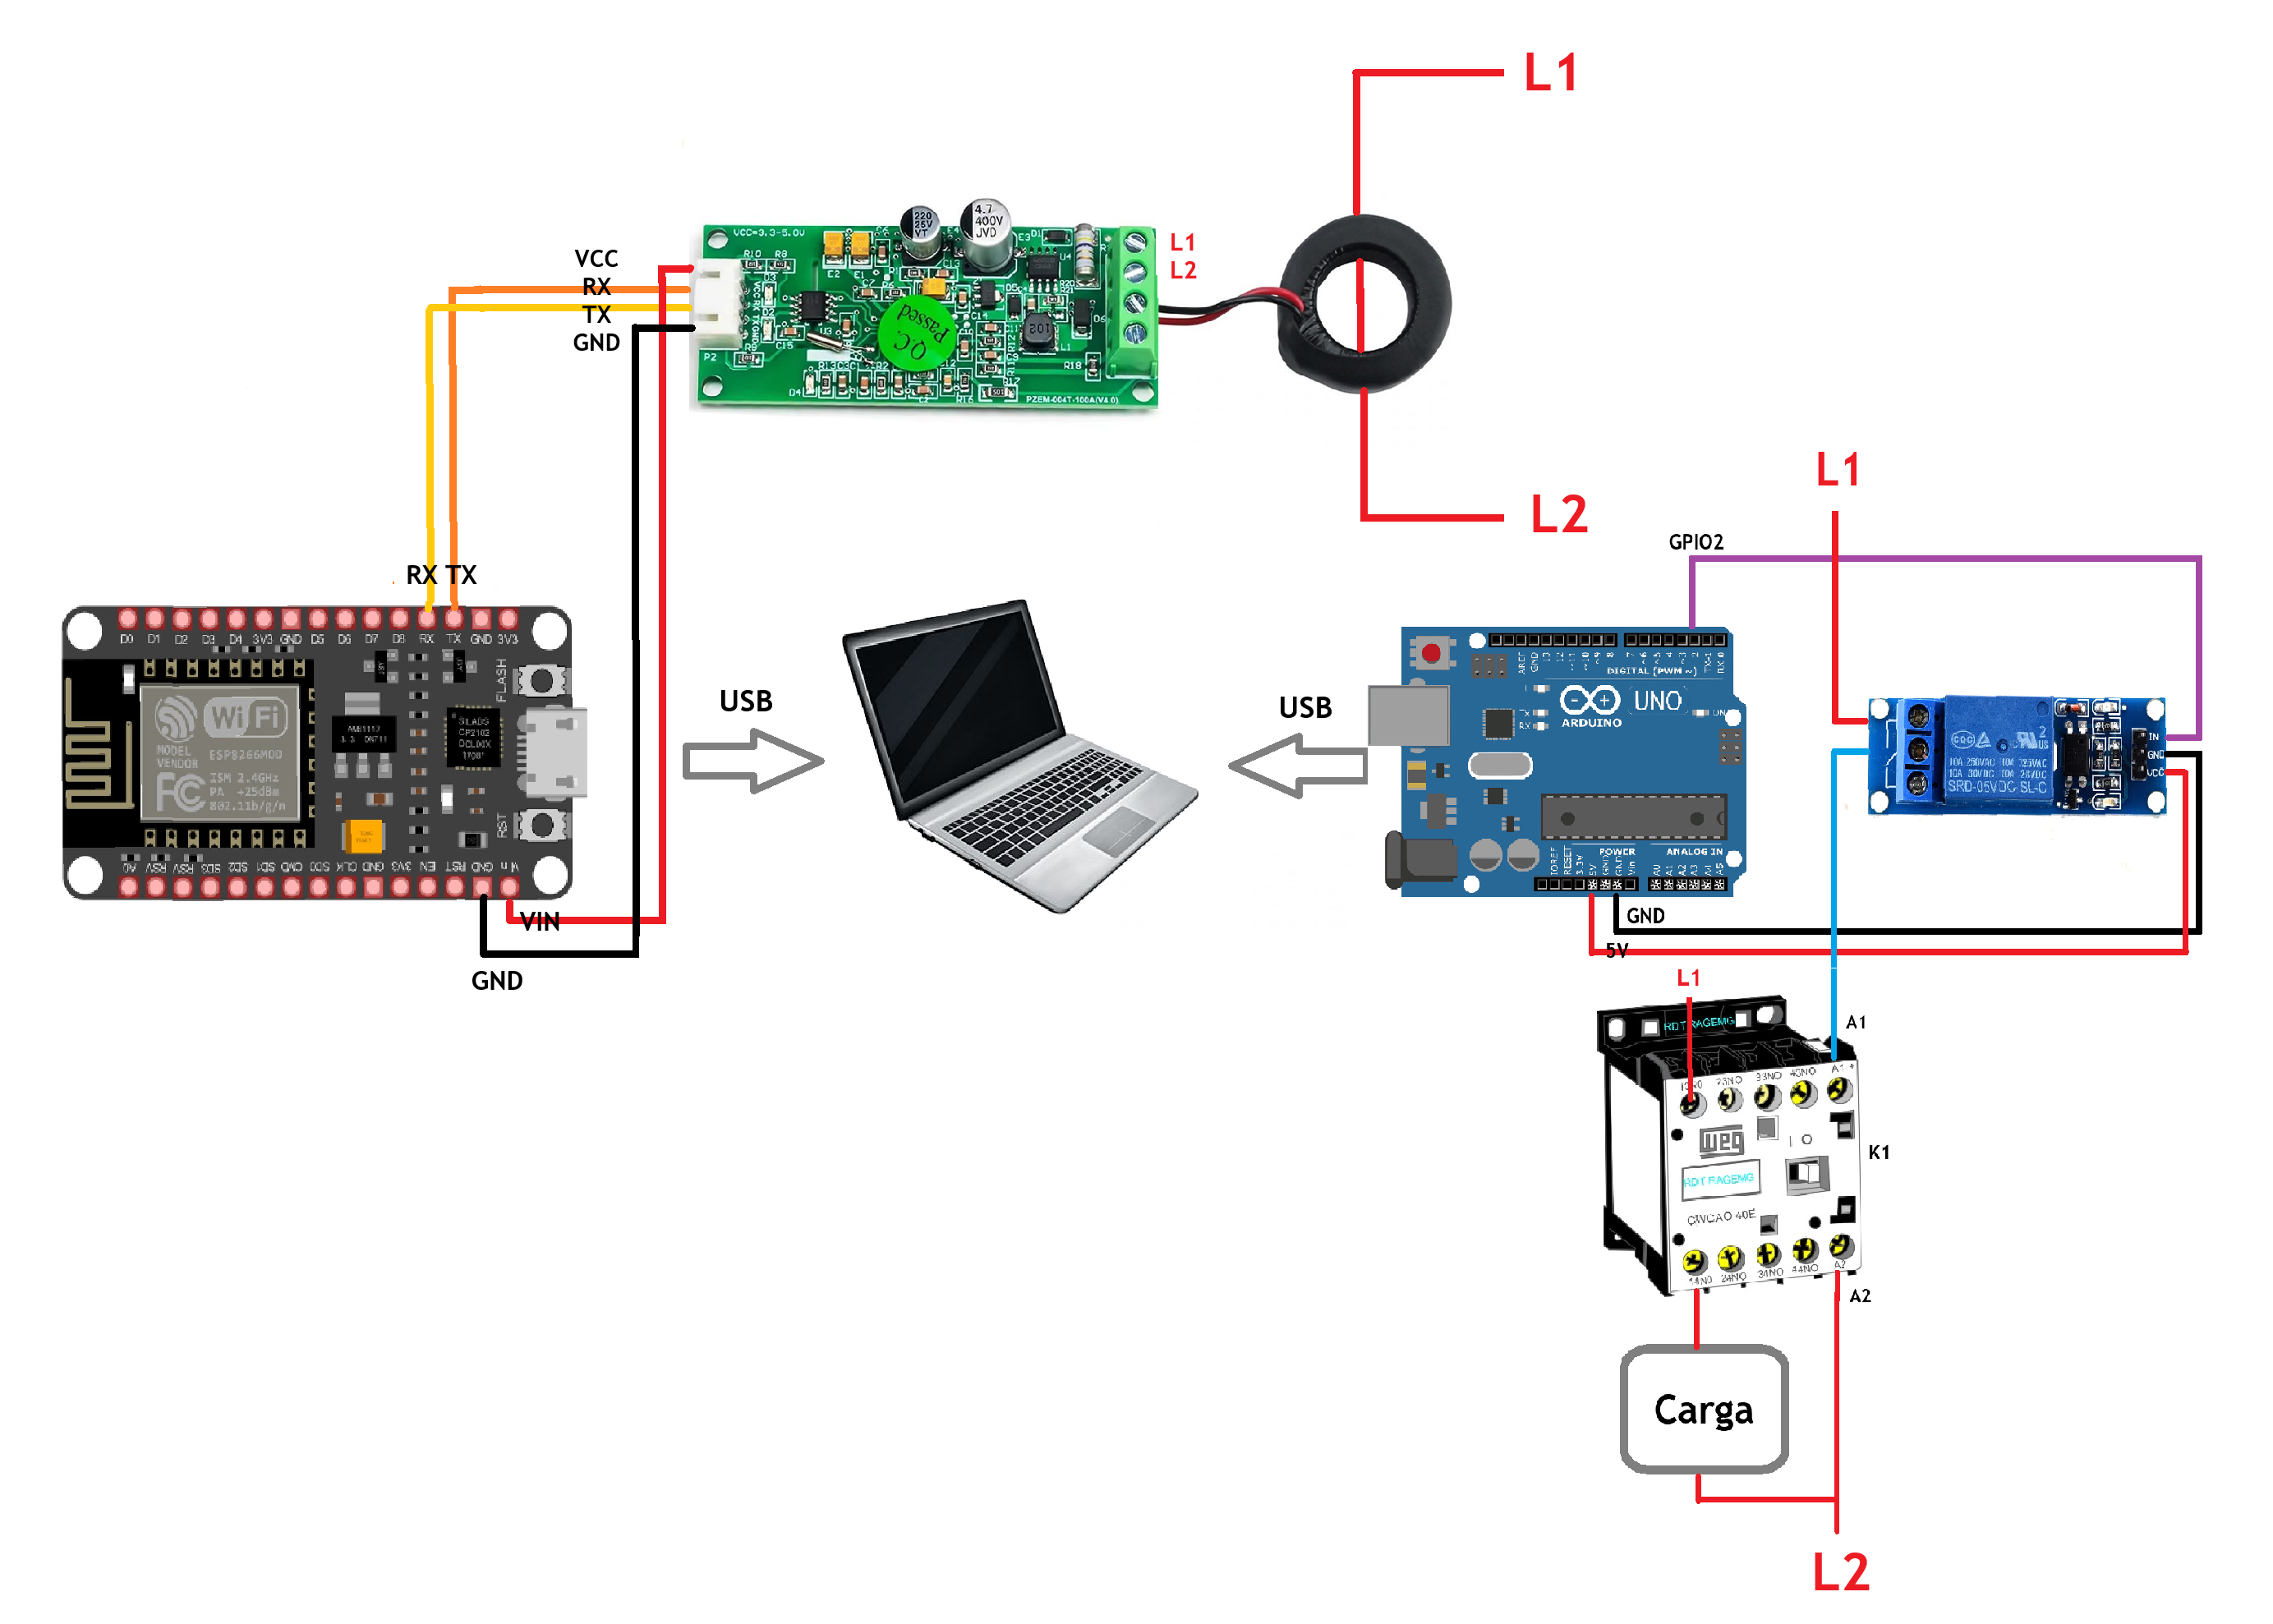
\includegraphics[width=1\textwidth]{Figuras/Esquematico_do_sistema (1).png} 
    \fonte{\me{2026}} 
    \label{fig:esquema_eletrico} 
\end{figure}

Essa arquitetura de conexão permitiu a leitura periódica das grandezas elétricas medidas pelo PZEM, possibilitando sua utilização tanto para armazenamento quanto para processamento pelos modelos implementados.

%------------------------------------------------------------------
%------------------------------------------------------------------
\section{Ambientes de Desenvolvimento e Implementação}

O Edge Impulse é uma plataforma de software especializada em soluções de Edge AI, voltada à simplificação do desenvolvimento e implantação de modelos de aprendizado de máquina, conforme ilustrado na Figura \ref{fig:edge_impulse}. A ferramenta oferece suporte completo ao ciclo de desenvolvimento de modelos de aprendizado de máquina, abrangendo etapas como aquisição de dados (com ou sem conectividade), pré-processamento, extração de características, treinamento, validação e exportação otimizada para execução em dispositivos ou ambientes de processamento \cite{STMicroelectronics}.

\begin{figure}[!htbp] 
    \centering
    \caption{Arquitetura da plataforma Edge Impulse.} 
    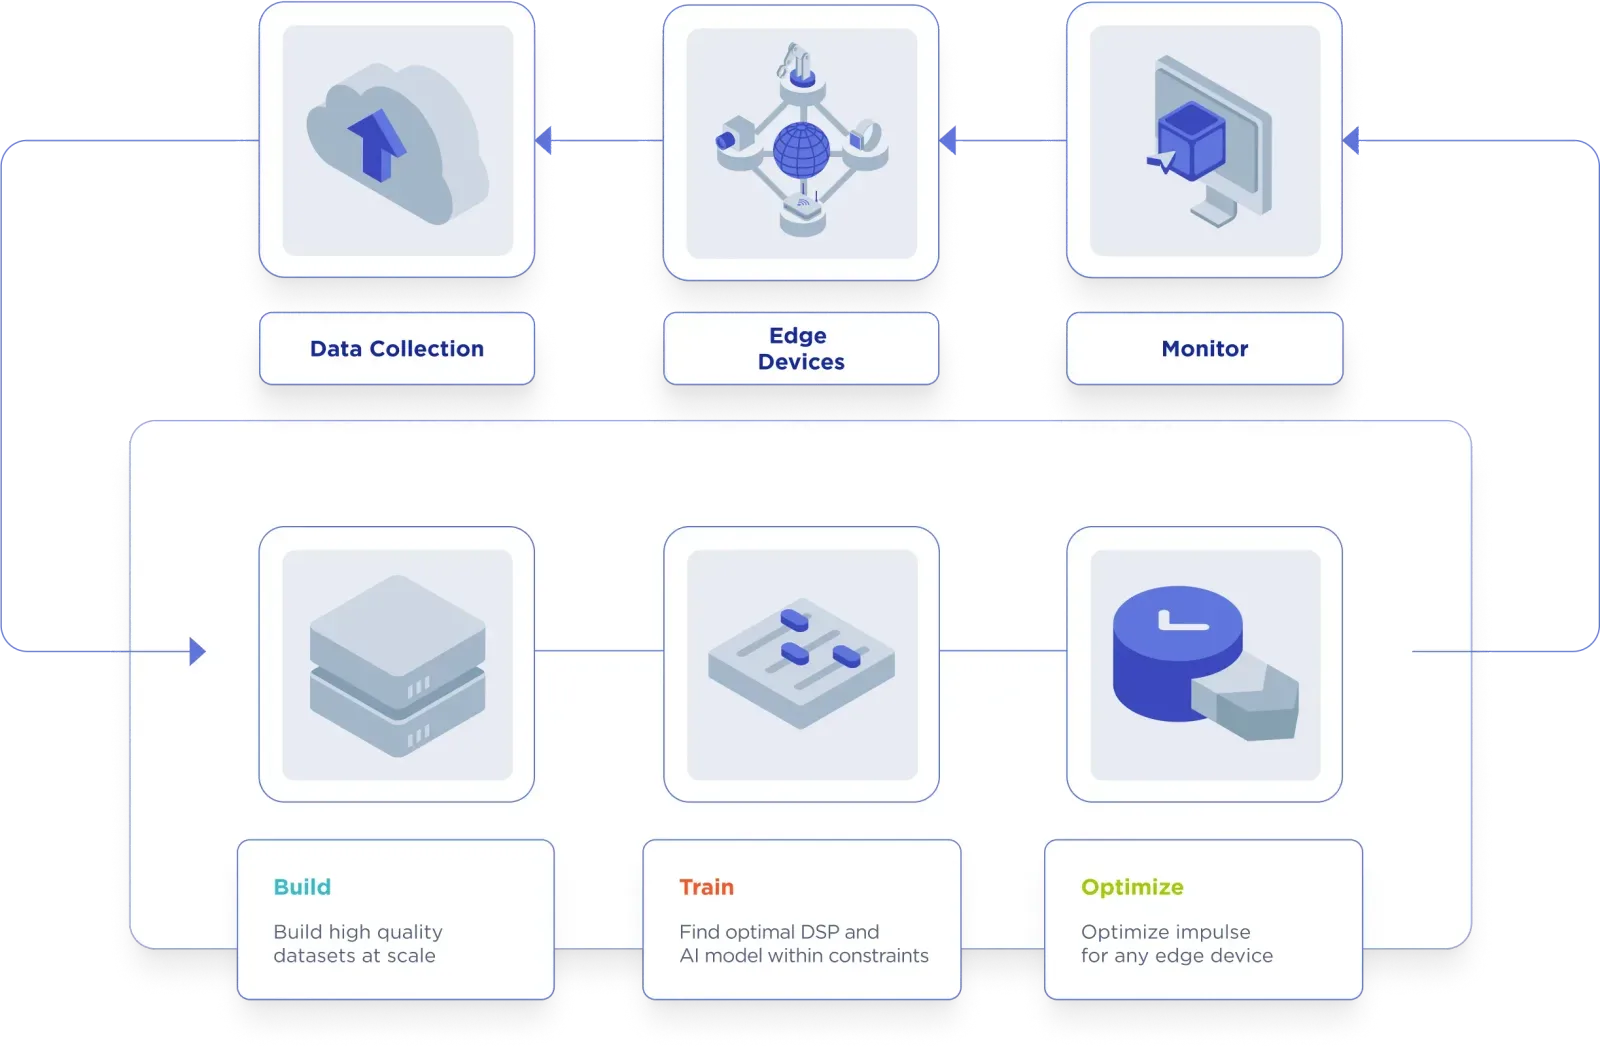
\includegraphics[width=1.0 \textwidth]{Figuras/Edge Impulse Diagrama.png} 
    \fonte{Figura extraída de \citeonline{STMicroelectronics}.} 
    \label{fig:edge_impulse} 
\end{figure}

Além da interface intuitiva e da facilidade de integração com diferentes plataformas de hardware e software, a ferramenta possibilita a realização de testes e otimizações utilizando dados reais, permitindo a identificação de inconsistências e ajustes no modelo antes de sua implantação final.

Neste trabalho, o Edge Impulse foi utilizado para a modelagem e treinamento de dois modelos baseados em redes neurais artificiais: um modelo de classificação, destinado à identificação do tipo de carga elétrica presente no sistema, e um modelo de regressão, utilizado para a estimativa do fator de potência (FP).

Os treinamentos dos modelos foram realizados em ambiente offline, utilizando dados históricos coletados durante os experimentos e previamente organizados em uma base de dados rotulada. A divisão do conjunto de dados em subconjuntos de treinamento e validação foi realizada dentro da própria plataforma Edge Impulse, permitindo a avaliação do desempenho dos modelos por meio de diferentes métricas. Após a etapa de treinamento e validação, os modelos foram exportados em formato compatível com execução em ambiente Node.js para integração no Node-RED.

O Node-RED foi utilizado para processamento e visualização dos dados em tempo real. No sistema proposto, a plataforma atua como cliente MQTT, conectando-se ao broker local para receber os dados medidos continuamente pelo sensor PZEM-004T e enviados pelo microcontrolador NodeMCU. Após o recebimento, os modelos exportados do Edge Impulse são executados no fluxo de processamento, realizando a inferência em tempo real e retornando os resultados, que são então exibidos em um dashboard web interativo desenvolvido para o acompanhamento das grandezas elétricas medidas e estimadas.

%------------------------------------------------------------------
\section{Modelagem e Treinamento dos Modelos}
\subsection{Geração da Base de Dados}
Para o treinamento dos modelos em ambiente Edge Impulse, foi necessário inicialmente construir uma base de dados rotulada representativa contendo as grandezas obtidas pelo sensor PZEM, bem como as grandezas derivadas calculadas a partir dessas medições, como potência aparente e potência reativa. Essas medições foram realizadas em bancada sob diferentes tipos de cargas em ambiente laboratorial controlado da Instituição.

Para essa etapa específica de aquisição de dados foi utilizado um microcontrolador Arduino Uno, empregado exclusivamente no controle das cargas, registro e armazenamento das medições em formato estruturado. Os códigos desenvolvidos para essa finalidade são apresentados nos Apêndices \ref{apendice_coleta_dados} e \ref{apendice_controle_cargas}.

Durante esse processo, os dados foram coletados em formato CSV, armazenados e organizados em uma planilha no \textit{Google Sheets}, apresentada no Apêndice \ref{apendice_google_sheets}, para posterior importação para o ambiente de treinamento dos modelos.

No total, foram coletadas 1000 amostras para cada tipo de carga, resultando em um conjunto de dados de 8000 amostras no total, para aplicação e avaliação dos modelos desenvolvidos. As classes de carga consideradas no processo de treinamento são apresentadas na Tabela \ref{tab_classes_carga}.

\begin{table}[!htbp]
    \centering
    \caption{Classes de carga utilizadas na base de dados}
    \label{tab_classes_carga}
    \begin{tabular}{|c|c|}
    \hline
    \textbf{Classe} & \textbf{Tipo de Carga} \\
    \hline
    0 & Sem carga \\
    \hline
    1 & Carga capacitiva \\
    \hline
    2 & Carga indutiva \\
    \hline
    3 & Carga resistiva \\
    \hline
    4 & Motor \\
    \hline
    5 & Cargas Resistiva + Capacitiva \\
    \hline
    6 & Cargas Resistiva + Indutiva \\
    \hline
    7 & Carga Capacitiva + Indutiva \\
    \hline
    \end{tabular}
    \fonte{\me{2026}}
\end{table}

\subsection{Pré-processamento dos Dados}

Antes do treinamento dos modelos, foi realizado o tratamento dos dados com o objetivo de melhorar a qualidade das informações fornecidas aos algoritmos de aprendizado de máquina.

Inicialmente, as variáveis de entrada foram submetidas a um processo de normalização utilizando o método \textit{StandardScaler}, que realiza a padronização com base na média e no desvio padrão da distribuição dos dados. Esse procedimento contribui para melhorar a convergência durante o treinamento das redes neurais. Posteriormente, o conjunto de dados foi dividido em dois subconjuntos: 80\% das amostras para treinamento e 20\% reservadas para teste e avaliação de desempenho.

\subsection{Configuração do Treinamento}
A Tabela \ref{tab_variaveis_modelo} apresenta as grandezas elétricas empregadas no treinamento dos modelos.

\begin{table}[!htbp]
    \centering
    \caption{Variáveis utilizadas no treinamento de cada modelo.}
    \label{tab_variaveis_modelo}
    \begin{tabular}{|c|c|c|}
    \hline
    \textbf{Modelo} & \textbf{Entradas}  & \textbf{Saídas} \\
    \hline
    Classificação & \makecell{Corrente, Potência Ativa, \\ Potência Aparente, Potência Reativa, \\ Fator de Potência} & Tipo de carga elétrica \\
    \hline
    Regressão & \makecell{Corrente, Potência Ativa, \\ Potência Aparente, Potência Reativa} & Fator de Potência \\
    \hline
    \end{tabular}
    \fonte{\me{2026}}
\end{table}


O treinamento foi realizado utilizando as ferramentas disponíveis na plataforma, com as seguintes configurações principais:
\begin{itemize}
    \item Número de épocas: 40
    \item Taxa de aprendizado (Learning rate): 0,0005
    \item Tamanho do conjunto de validação: 20\%
\end{itemize}

\subsection{Arquitetura da Rede Neural}

Os modelos de classificação e regressão foram implementados utilizando arquiteturas semelhantes de redes neurais do tipo MLP. Cada modelo é composto por uma camada de entrada correspondente às variáveis elétricas medidas, duas camadas intermediárias e uma camada de saída. A Tabela \ref{tab:arquitetura_modelos} apresenta a quantidade de neurônios utilizadas nas camadas de cada modelo.

\begin{table}[!htbp]
    \centering
    \caption{Arquitetura dos modelos de classificação e regressão.}
    \label{tab:arquitetura_modelos}
    \begin{tabular}{|c|c|c|}
    \hline
    \textbf{Camada} & \textbf{Classificação} & \textbf{Regressão} \\
    \hline
    Entrada & 5 & 4 \\
    \hline
    Oculta 1 & 20 & 20 \\
    \hline
    Oculta 2 & 30 & 30 \\
    \hline
    Saída & 8 & 1 \\
    \hline
    \end{tabular}
    \fonte{\me{2026}}
\end{table}

%------------------------------------------------------------------
%------------------------------------------------------------------
\section{Cenários de Aplicação e Validação dos Modelos}

As medições do sensor PZEM-004T foram lidas pelo microcontrolador NodeMCU ESP8266 e publicadas periodicamente no broker MQTT a cada 1 segundo em um tópico único denominado \textit{pzem/dados} no ambiente de processamento Node-RED. Para isso, foi necessário configurar as credenciais da rede Wi-Fi e do servidor MQTT utilizados para estabelecer a comunicação com o broker da aplicação. O código de integração entre o sensor PZEM-004T e o NodeMCU é apresentado no Apêndice \ref{cod_integracao_PZEM_MQTT}. 

Para a comunicação com o sensor foi utilizada a biblioteca \textit{PZEM004Tv30}, responsável por realizar a interface serial com o módulo de medição elétrica por meio da porta UART padrão do microcontrolador (GPIO1 e GPIO3). O programa também foi responsável por formatar os dados em um objeto no formato JSON para uso no Node-RED.

\subsection{Processamento no ambiente Node-RED}
Conforme apresentado na Figura \ref{fig:Nó edge-impulse-classify}, o ambiente Node-RED foi configurado como a camada responsável pelo processamento, integração e visualização do sistema, recebendo os dados enviados pelo microcontrolador via protocolo MQTT e executando os resultados dos modelos.

\begin{figure}[!htbp] 
    \centering
    \caption{Configuração do ambiente Node-RED.} 
    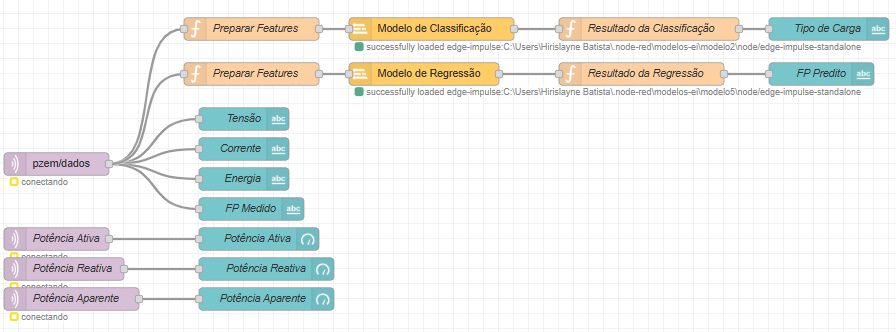
\includegraphics[width = 1\textwidth]{Figuras/Configuracao do Dashboard.png} 
    \fonte{\me{2026}} 
    \label{fig:Nó edge-impulse-classify} 
\end{figure}

As principais funcionalidades implementadas no fluxo de processamento são apresentadas na Tabela \ref{tab_fluxo_nodered}.

\begin{table}[!htbp]
    \centering
    \caption{Componentes do fluxo de processamento no Node-RED}
    \label{tab_fluxo_nodered}
    \begin{tabular}{|p{2.5cm}|p{5.5cm}|p{5.5cm}|}
    \hline
    \multicolumn{1}{|c|}{\textbf{Módulo}} & \multicolumn{1}{c|}{\textbf{Componente}} & \multicolumn{1}{c|}{\textbf{Função}} \\
    \hline
    Recepção & Nó MQTT IN (tópico \textit{pzem/dados}) & Recebe o JSON com todas as medições do sensor \\
    \hline
    Preparação & Nó Function \textit{Preparar Features} & Extrai e organiza as variáveis de entrada do modelo \\
    \hline
    Classificação e Estimativa & Nó \textit{edge-impulse-classify} & Executa o modelo \textit{WebAssembly} em tempo real \\
    \hline
    Processamento & Nós Functions \textit{Resultado da Classificação} e \textit{Resultado da Regressão} & Formatam os valores gerados pelos modelos para melhor visualização\\
    \hline
    Visualização & Nós \textit{text} e \textit{gauge} UI & Exibe medições, classificações e estimativas em tempo real \\
    \hline
    \end{tabular}
    \fonte{\me{2026}}
\end{table}

O nó \textit{Function} denominado \textit{Preparar Features} foi configurado para extrair do objeto JSON recebido via MQTT as variáveis necessárias para os modelos, organizando-as na mesma ordem utilizada durante o treinamento no Edge Impulse, conforme códigos apresentados em \ref{cod_preparacao_features_modelo_class} e \ref{cod_preparacao_features_modelo_regr}.

\begin{lstlisting}[language=JavaScript, caption={Preparação das variáveis de entrada para o modelo de classificação.}, label={cod_preparacao_features_modelo_class}]
    let dados = msg.payload;
    msg.payload = [
        Number(dados.corrente),
        Number(dados.potencia),
        Number(dados.aparente),
        Number(dados.reativa),
        Number(dados.fp)
    ];
    msg.dados = dados;
    return msg;
\end{lstlisting}

\begin{lstlisting}[language=JavaScript, caption={Preparação das variáveis de entrada para o modelo de regressão.}, label={cod_preparacao_features_modelo_regr}]
    let dados = msg.payload;
    msg.payload = [
        Number(dados.corrente),
        Number(dados.potencia),
        Number(dados.aparente),
        Number(dados.reativa)
    ];
    msg.dados = dados;
    return msg;
\end{lstlisting}

O nó \textit{edge-impulse-classify} foi configurado para executar cada um dos modelos. Para isso, basta copiar o caminho do diretório exportado do \textit{Edge Impulse} que contém os arquivos \textit{edge-impulse-standalone.js} e \textit{.wasm}, responsáveis pela execução do modelo de rede neural, e armazená-lo no diretório local do Node-RED, conforme a ilustrado na Figura \ref{fig:Nó edge-impulse-classify}.

\begin{figure}[!htbp] 
    \centering
    \caption{Configuração do nó \textit{edge-impulse-classify}.} 
    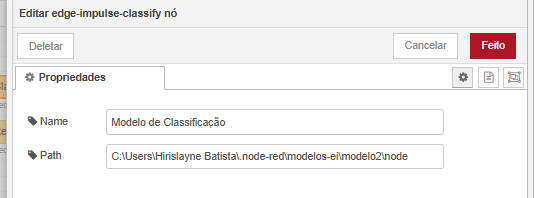
\includegraphics[width = 1\textwidth]{Figuras/Nó edge-impulse-classify.png} 
    \fonte{\me{2026}} 
    \label{fig:Nó edge-impulse-classify} 
\end{figure}

A cada novo conjunto de dados recebido, os nós executam o processo de inferência e retornam as probabilidades associadas a cada uma das oito classes de carga e o valor do FP estimado, respectivamente, enviando esses valores para os nós de função seguintes, denominados \textit{Resultado da Classificação} e \textit{Resultado da Regressão}.  Esses resultados são então enviados para os nós de função seguintes, denominados \textit{Resultado da Classificação} e \textit{Resultado da Regressão}, que interpretam e formatam as saídas para o dashboard. Os códigos referentes a essas funções são apresentados em \ref{cod_resultado_classificacao} e \ref{cod_resultado_regressao}.

\begin{lstlisting}[language=JavaScript, caption={Processamento da saída do modelo de classificação}, label={cod_resultado_classificacao}]
    // recebe a saida do Edge Impulse
    let resultados = msg.payload.results;
    
    // cria um texto formatado para o dashboard
    let classe = "";
    let maior = 0;
    
    // percorre todas as classes
    for (let i = 0; i < resultados.length; i++) {
        if (resultados[i].value > maior) {
            maior = resultados[i].value;
            classe = resultados[i].label;
        }
    }
    
    let nomes = {
        "0": "Sem carga",
        "1": "Capacitiva",
        "2": "Indutiva",
        "3": "Resistiva",
        "4": "Motor",
        "5": "Resistiva + Capacitiva",
        "6": "Resisitiva + Indutiva",
        "7": "Capacitiva + Indutiva"
    };
    
    msg.payload = nomes[classe];
    return msg;
\end{lstlisting}

\begin{lstlisting}[language=JavaScript, caption={Processamento da saída do modelo de regressão.}, label={cod_resultado_regressao}]
    let resultados = msg.payload.results;
    let valor = 0;
    valor = resultados[0].value;
    
    msg.payload = valor;
    return msg;
\end{lstlisting}

Por fim, as medições e os resultados dos modelos foram disponibilizados em um painel de monitoramento desenvolvido na plataforma Node-RED, conforme exemplo ilustrado na Figura \ref{fig:painel-monitoramento}. Esse painel permite a visualização em tempo real das grandezas medidas pelo sensor, da classe de carga identificada e do fator de potência estimado, por meio de elementos visuais como gráficos e indicadores textuais.

\begin{figure}[!htbp] 
    \centering
    \caption{ Painel de monitoramento Node-RED.} 
    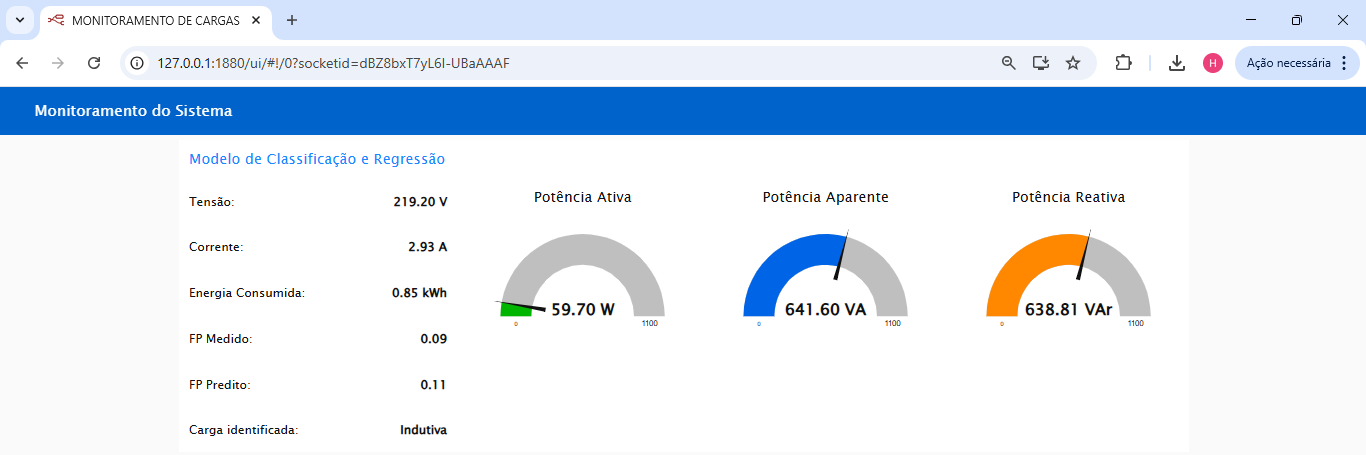
\includegraphics[width = 1\textwidth]{Figuras/tela_carga_indutiva.png} 
    \fonte{\me{2026}} 
    \label{fig:painel-monitoramento} 
\end{figure}    % Metodologia
 %-------------
% Resultados e Discussão
%--------------------------
\chapter{Resultados e Discussão} \label{Resultados e Discussão}

Este capítulo apresenta os resultados obtidos ao longo do trabalho, abrangendo uma breve análise da dispersão da base de dados experimental, o desempenho dos modelos de classificação e regressão desenvolvidos e a validação experimental do sistema proposto em tempo real.

% ---------------------------------------------------------------------------
\section{Base experimental coletada}
A Figura \ref{fig:dispersao_potencia_corrente} apresenta um gráfico de dispersão entre corrente elétrica e potência ativa para as amostras coletadas. Observa-se a formação de agrupamentos distintos de pontos associados aos diferentes tipos de carga, indicando que essas grandezas apresentam padrões característicos para cada configuração analisada.

Esse comportamento evidencia que as variáveis elétricas medidas possuem forte capacidade discriminativa, o que favorece o processo de aprendizado do modelo de classificação. Dessa forma, os dados experimentais apresentam separabilidade significativa no espaço de características, contribuindo para o elevado desempenho obtido pelos modelos de aprendizado de máquina. O código desenvolvido dessa análise está disponível no Apêndice \ref{apendice_análise_PZEM}.

\begin{figure}[!htbp]
    \centering
    \caption{Gráfico de dispersão entre corrente e potência ativa das amostras coletadas.}
    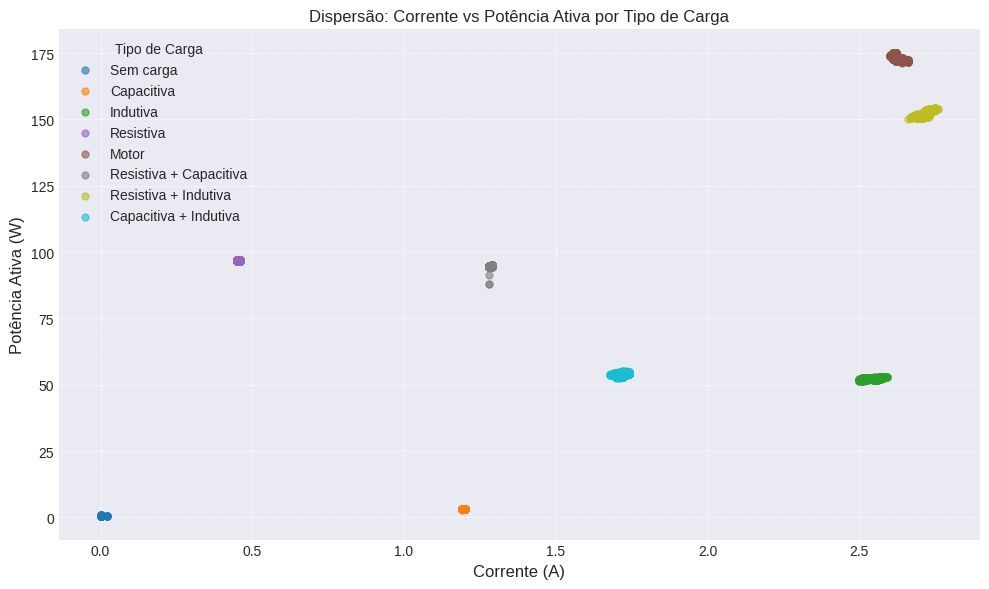
\includegraphics[width=1\textwidth]{Figuras/grafico de dispersao I vs P por tipo de carga.png}
    \fonte{\me{2026}}
    \label{fig:dispersao_potencia_corrente}
\end{figure}

% ---------------------------------------------------------------------------
\section{Desempenho do modelo de classificação}
O desempenho do modelo de classificação foi avaliado por meio das métricas de acurácia, precisão, \textit{recall} e \textit{F1-score}, além da análise da matriz de confusão obtida no conjunto de teste. O treinamento foi conduzido por 40 épocas, com monitoramento da perda (\textit{loss}) e acurácia tanto para os conjuntos de treinamento quanto de validação.

Observa-se que o modelo atingiu acurácia de 100\% no treinamento a partir da época 29, com valores de perda próximos de zero (\textit{val\_loss} de 0,0048 ao final do treinamento). Os resultados de precisão, recall e F1-score foram iguais a 1,0 para todas as classes avaliadas, indicando que o erro do modelo foi praticamente nulo (inferior a 0,5\% ao final das 40 épocas). A Figura \ref{fig:graficos_modelo_classificacao} apresenta a evolução da acurácia e da perda ao longo das épocas de treinamento. 

A matriz de confusão apresentada na Figura \ref{fig:matriz_confusao} demonstra que todas as amostras foram corretamente classificadas pelo modelo, sem ocorrência de erros entre as categorias de carga. A diagonal principal da matriz apresenta valores máximos para todas as classes, confirmando a eficácia do modelo em distinguir os diferentes tipos de carga analisados.

\begin{figure}[!htbp]
    \centering
    \caption{Matriz de confusão do modelo de classificação de cargas.}
    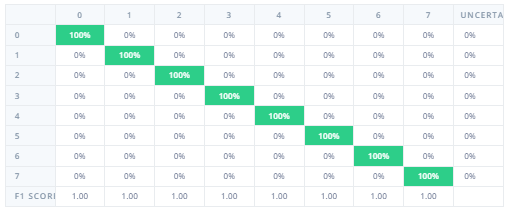
\includegraphics[width=\textwidth]{Figuras/matriz de confusao modelo de classificacao.png}
    \fonte{\me{2026}}
    \label{fig:matriz_confusao}
\end{figure}

Esses resultados evidenciam que as variáveis elétricas utilizadas como entrada apresentam forte capacidade de distinção entre os diferentes tipos de carga analisados. Além disso, a separabilidade observada nos dados experimentais, conforme demonstrado na Figura \ref{fig:dispersao_potencia_corrente}, contribuiu significativamente para facilitar o processo de aprendizado da rede neural, permitindo que o modelo convergisse rapidamente para uma solução ótima.

\begin{figure}[h]
    \centering
    \caption{Métricas de desempenho do modelo de classificação ao longo das épocas de treinamento.}
    \subfigure[Evolução da acurácia.]{
        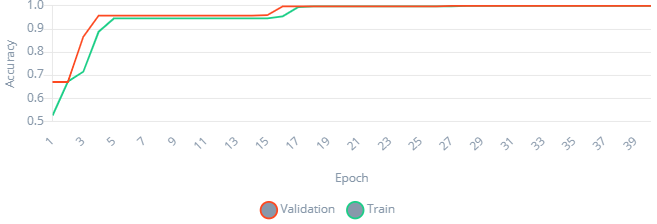
\includegraphics[width=0.9\textwidth]{Figuras/grafico de acuracia modelo classificacao.png}
    }
    \hfill
    \subfigure[Evolução da perda (loss).]{
        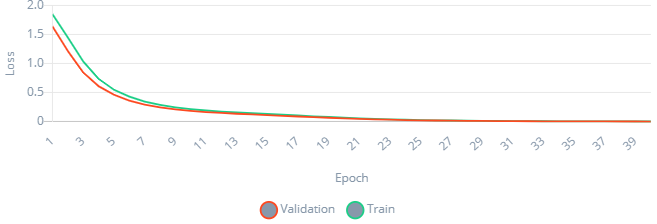
\includegraphics[width=0.9\textwidth]{Figuras/grafico de erro modelo de classificacao.png}
    }
    \hfill
    \subfigure[Evolução do treinamento do modelo.]{
        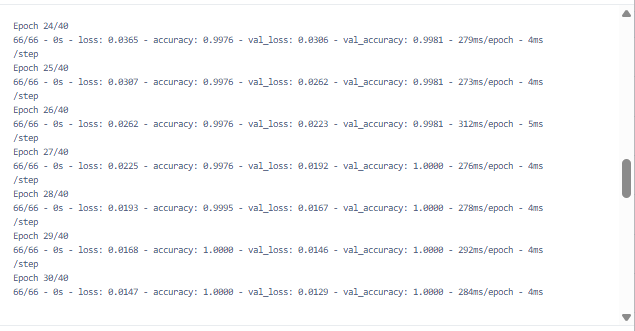
\includegraphics[width=0.9\textwidth]{Figuras/treinamento modelo classificao.png}
    }
    \fonte{\me{2026}} 
    \label{fig:graficos_modelo_classificacao}
\end{figure}

% ---------------------------------------------------------------------------
\section{Desempenho do modelo de regressão}
O desempenho do modelo de regressão foi avaliado utilizando as métricas de erro quadrático médio (MSE) e erro absoluto médio (MAE), além da análise da evolução da perda durante o treinamento. A Figura \ref{fig:graficos_modelo_regressao} apresenta a evolução do erro ao longo das épocas de treinamento. Observa-se que o modelo convergiu rapidamente, atingindo valores de perda próximos de zero já nas primeiras épocas. Ao final do treinamento, os valores de perda estabilizaram-se em torno de $0,94967 \times 10^{-5}$ para o treinamento e $3,3 \times 10^{-5}$ para a validação.

\begin{figure}[h]
    \centering
    \caption{Métricas de desempenho do modelo de regressão ao longo das épocas de treinamento.}
    \subfigure[Evolução da perda (loss).]{
        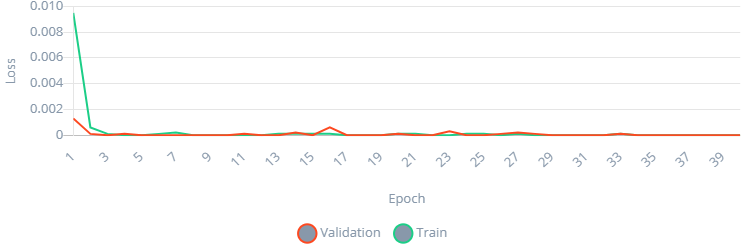
\includegraphics[width=0.9\textwidth]{Figuras/grafico de erro modelo de regressao.png}
    }
    \hfill
    \subfigure[Evolução do treinamento do modelo.]{
        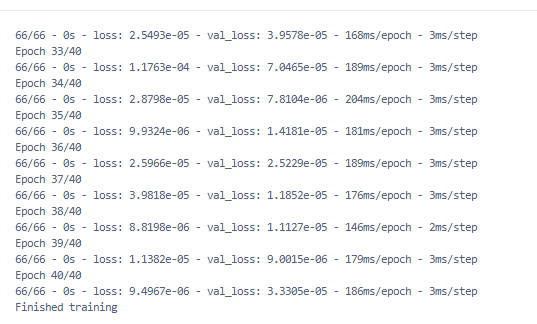
\includegraphics[width=0.7\textwidth]{Figuras/treinamento modelo regressão.png}
    }
    \fonte{\me{2026}}
    \label{fig:graficos_modelo_regressao}
\end{figure}


No conjunto de teste, o modelo apresentou MSE de $8,3 \times 10^{-6}$ e MAE de 0,00228, indicando elevada precisão na estimação do fator de potência. O coeficiente de variância explicada (\textit{explained variance score}) atingiu 0,9997, demonstrando que o modelo é capaz de explicar 99,97\% da variância dos dados, o que evidencia um excelente ajuste.

A Tabela \ref{tab:metricas_regressao} resume as principais métricas de desempenho obtidas pelo modelo nos conjuntos de validação e teste.

\begin{table}[h]
    \centering
    \caption{Métricas de desempenho do modelo de regressão.}
    \label{tab:metricas_regressao}
    \begin{tabular}{lccc}
    \hline
    \textbf{Conjunto} & \textbf{MSE} & \textbf{MAE} & \textbf{Variância Explicada} \\
    \hline
    Validação (float32) & $7,81 \times 10^{-6}$ & 0,00224 & 0,99972 \\
    Teste (float32) & $8,30 \times 10^{-6}$ & 0,00228 & 0,99970 \\
    \hline
    \end{tabular}
    \fonte{\me{2026}}
\end{table}

Os resultados obtidos demonstram que o modelo de regressão é capaz de estimar o fator de potência com erro extremamente baixo, sendo que essa precisão é atribuída principalmente à qualidade dos dados experimentais.

% ---------------------------------------------------------------------------
\section{Validação do sistema em tempo real}
% O sistema foi implementado em bancada experimental, integrando sensor PZEM-004T, microcontrolador NodeMCU ESP8266, relés, contatores, medidor de referência e as seguintes cargas: lâmpada, transformador, três capacitores de 5 $\mu$F em paralelo e motor de indução. A Figura \ref{fig:sistema_montado} ilustra a configuração utilizada nos testes.

O sistema foi implementado em bancada experimental, integrando sensor PZEM-004T, microcontrolador NodeMCU ESP8266, Arduino Uno, módulos relé, contatores, medidor de referência e as seguintes cargas: lâmpada (carga resistiva), transformador (carga indutiva), três capacitores de 5 $\mu$F em paralelo (carga capacitiva) e motor de indução. A Figura \ref{fig:sistema_montado} ilustra a configuração utilizada nos testes.

A Figura \ref{fig:sistema_montado}(a) apresenta o sistema de cargas, composto pelos contatores, medidor de referência e os elementos de carga utilizados nos experimentos. Já a Figura \ref{fig:sistema_montado}(b) mostra o sistema de aquisição, transmissão e controle, destacando o sensor PZEM-004T, o microcontrolador NodeMCU ESP8266, o Arduino Uno utilizado no controle dos relés e os módulos relé responsáveis pelo acionamento das cargas.

\begin{figure}[h]
    \centering
    \caption{Sistema experimental desenvolvido para aquisição e monitoramento das grandezas elétricas.}
    \subfigure[Sistema de cargas.]{
        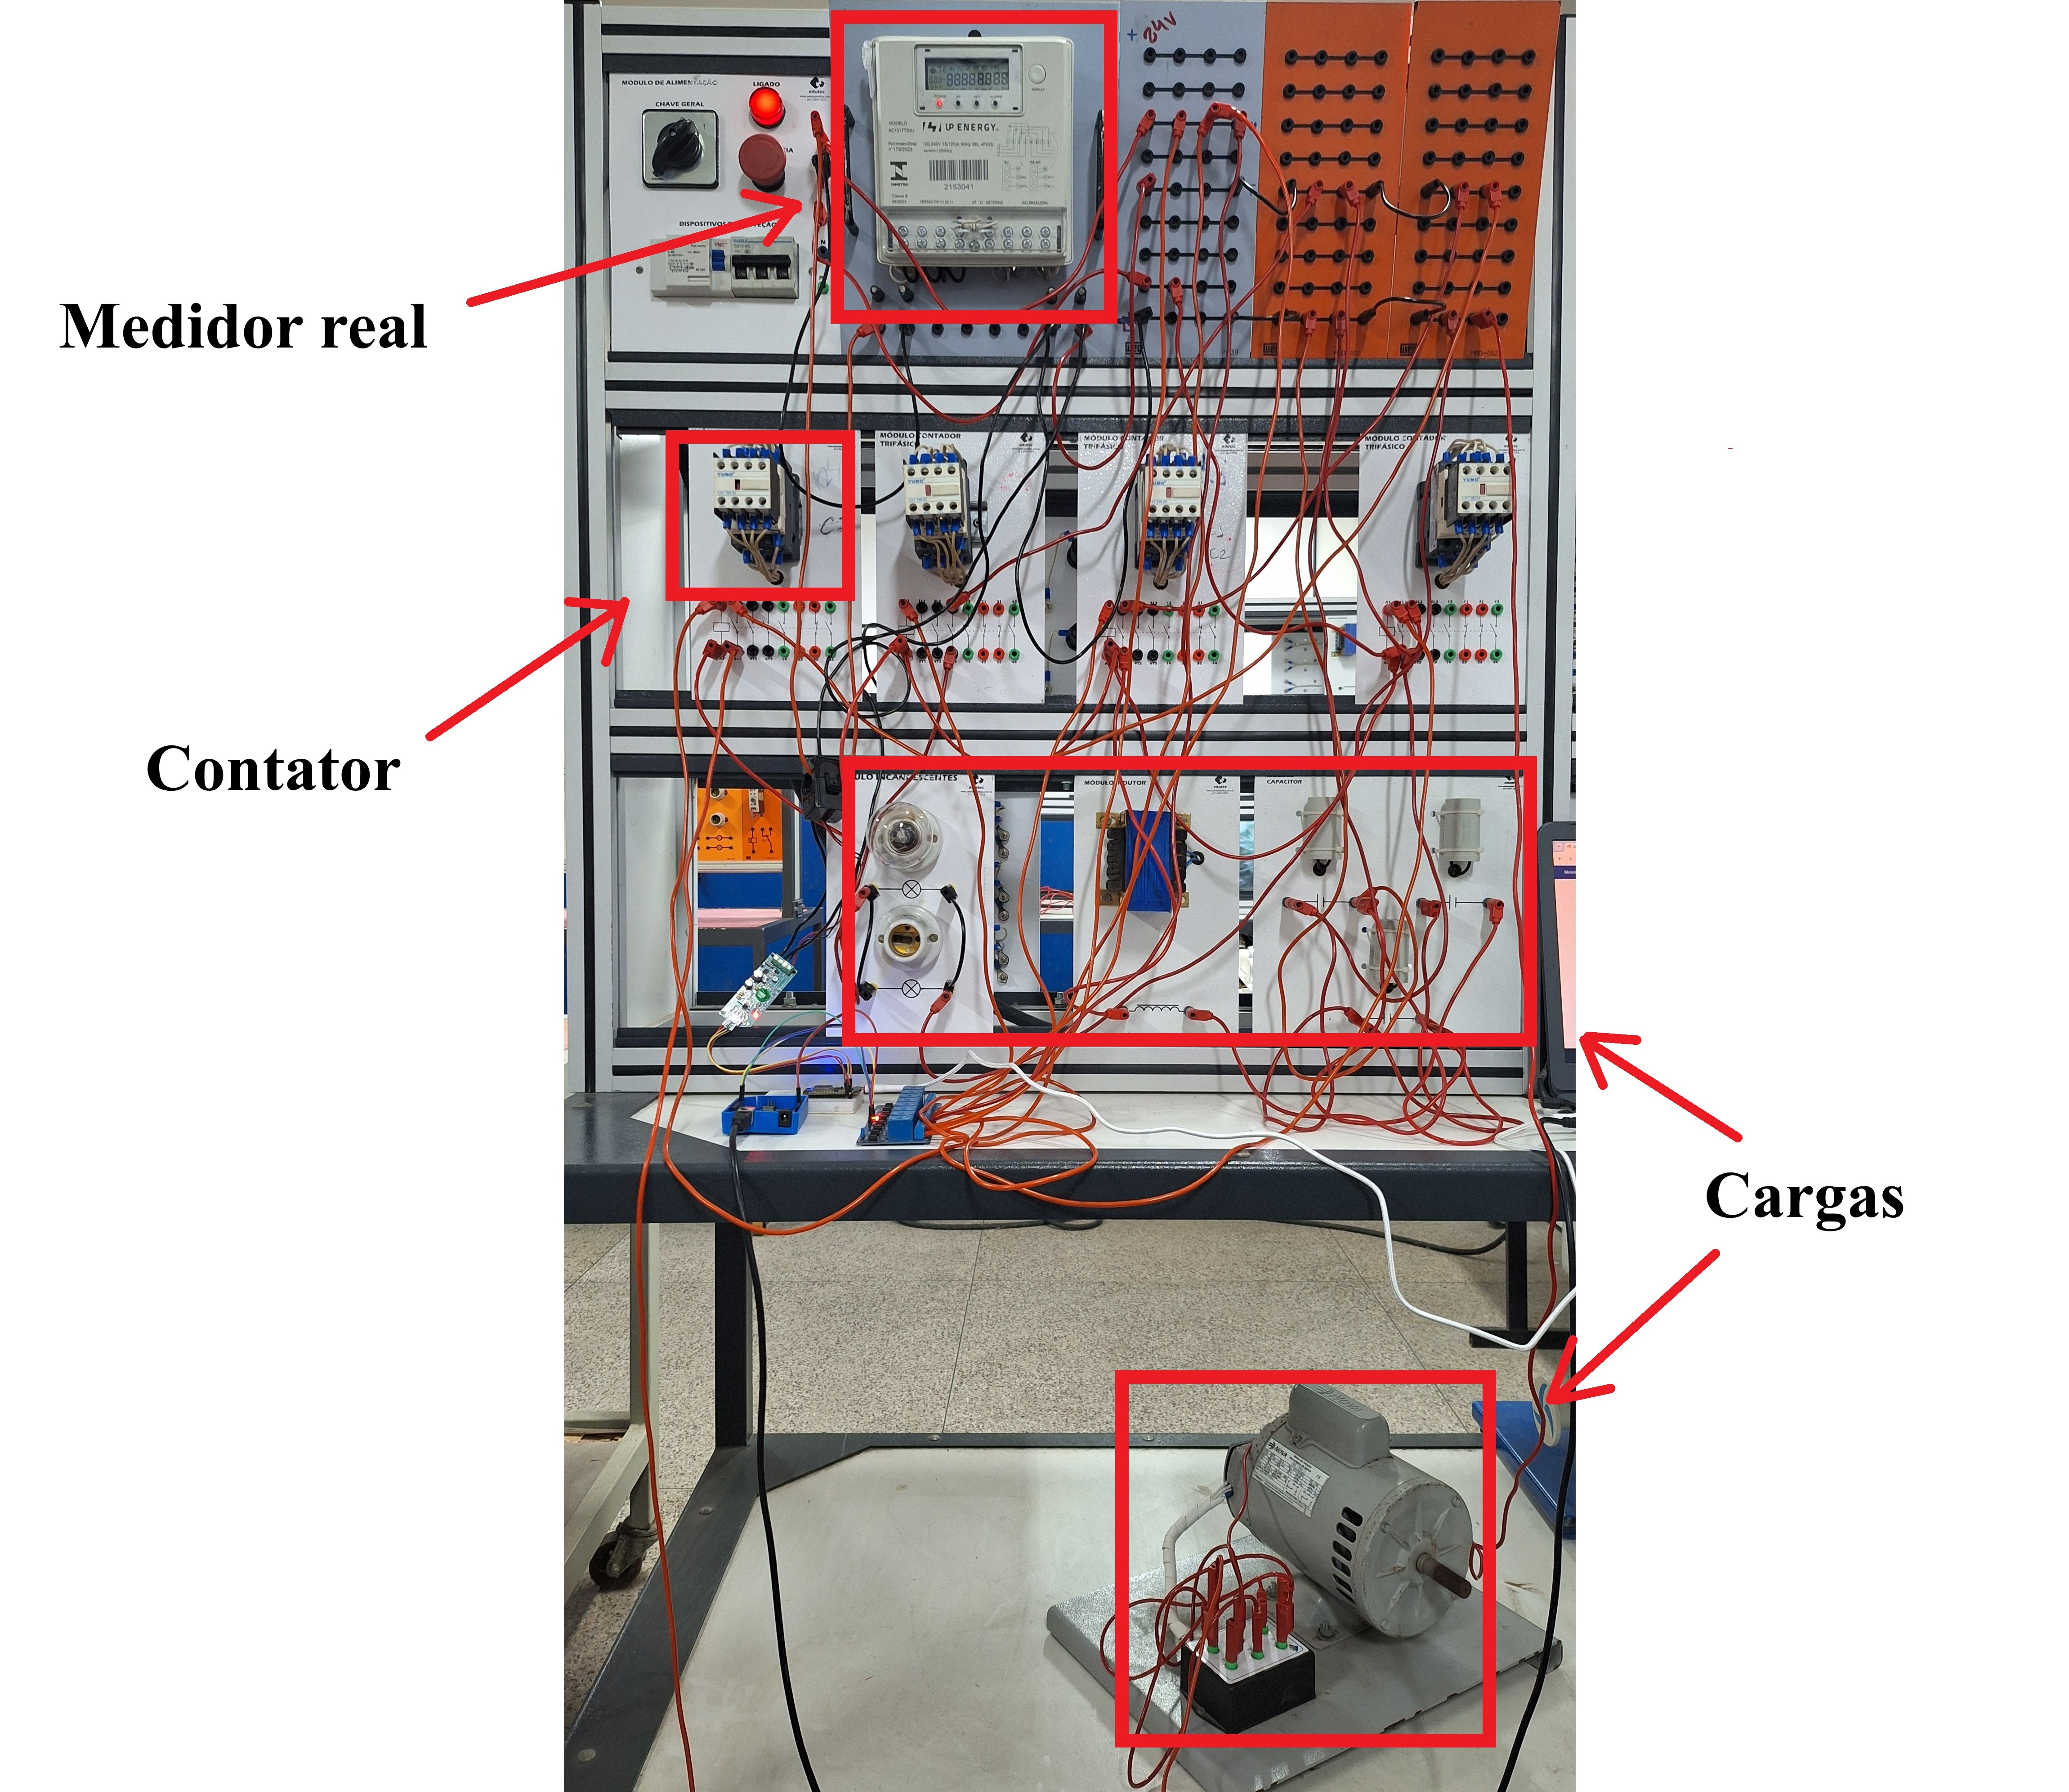
\includegraphics[width=0.8\textwidth]{Figuras/Sistema-montado.jpg}
    }
    \hfill
    \subfigure[Sistema de aquisição, transmissão e controle.]{
        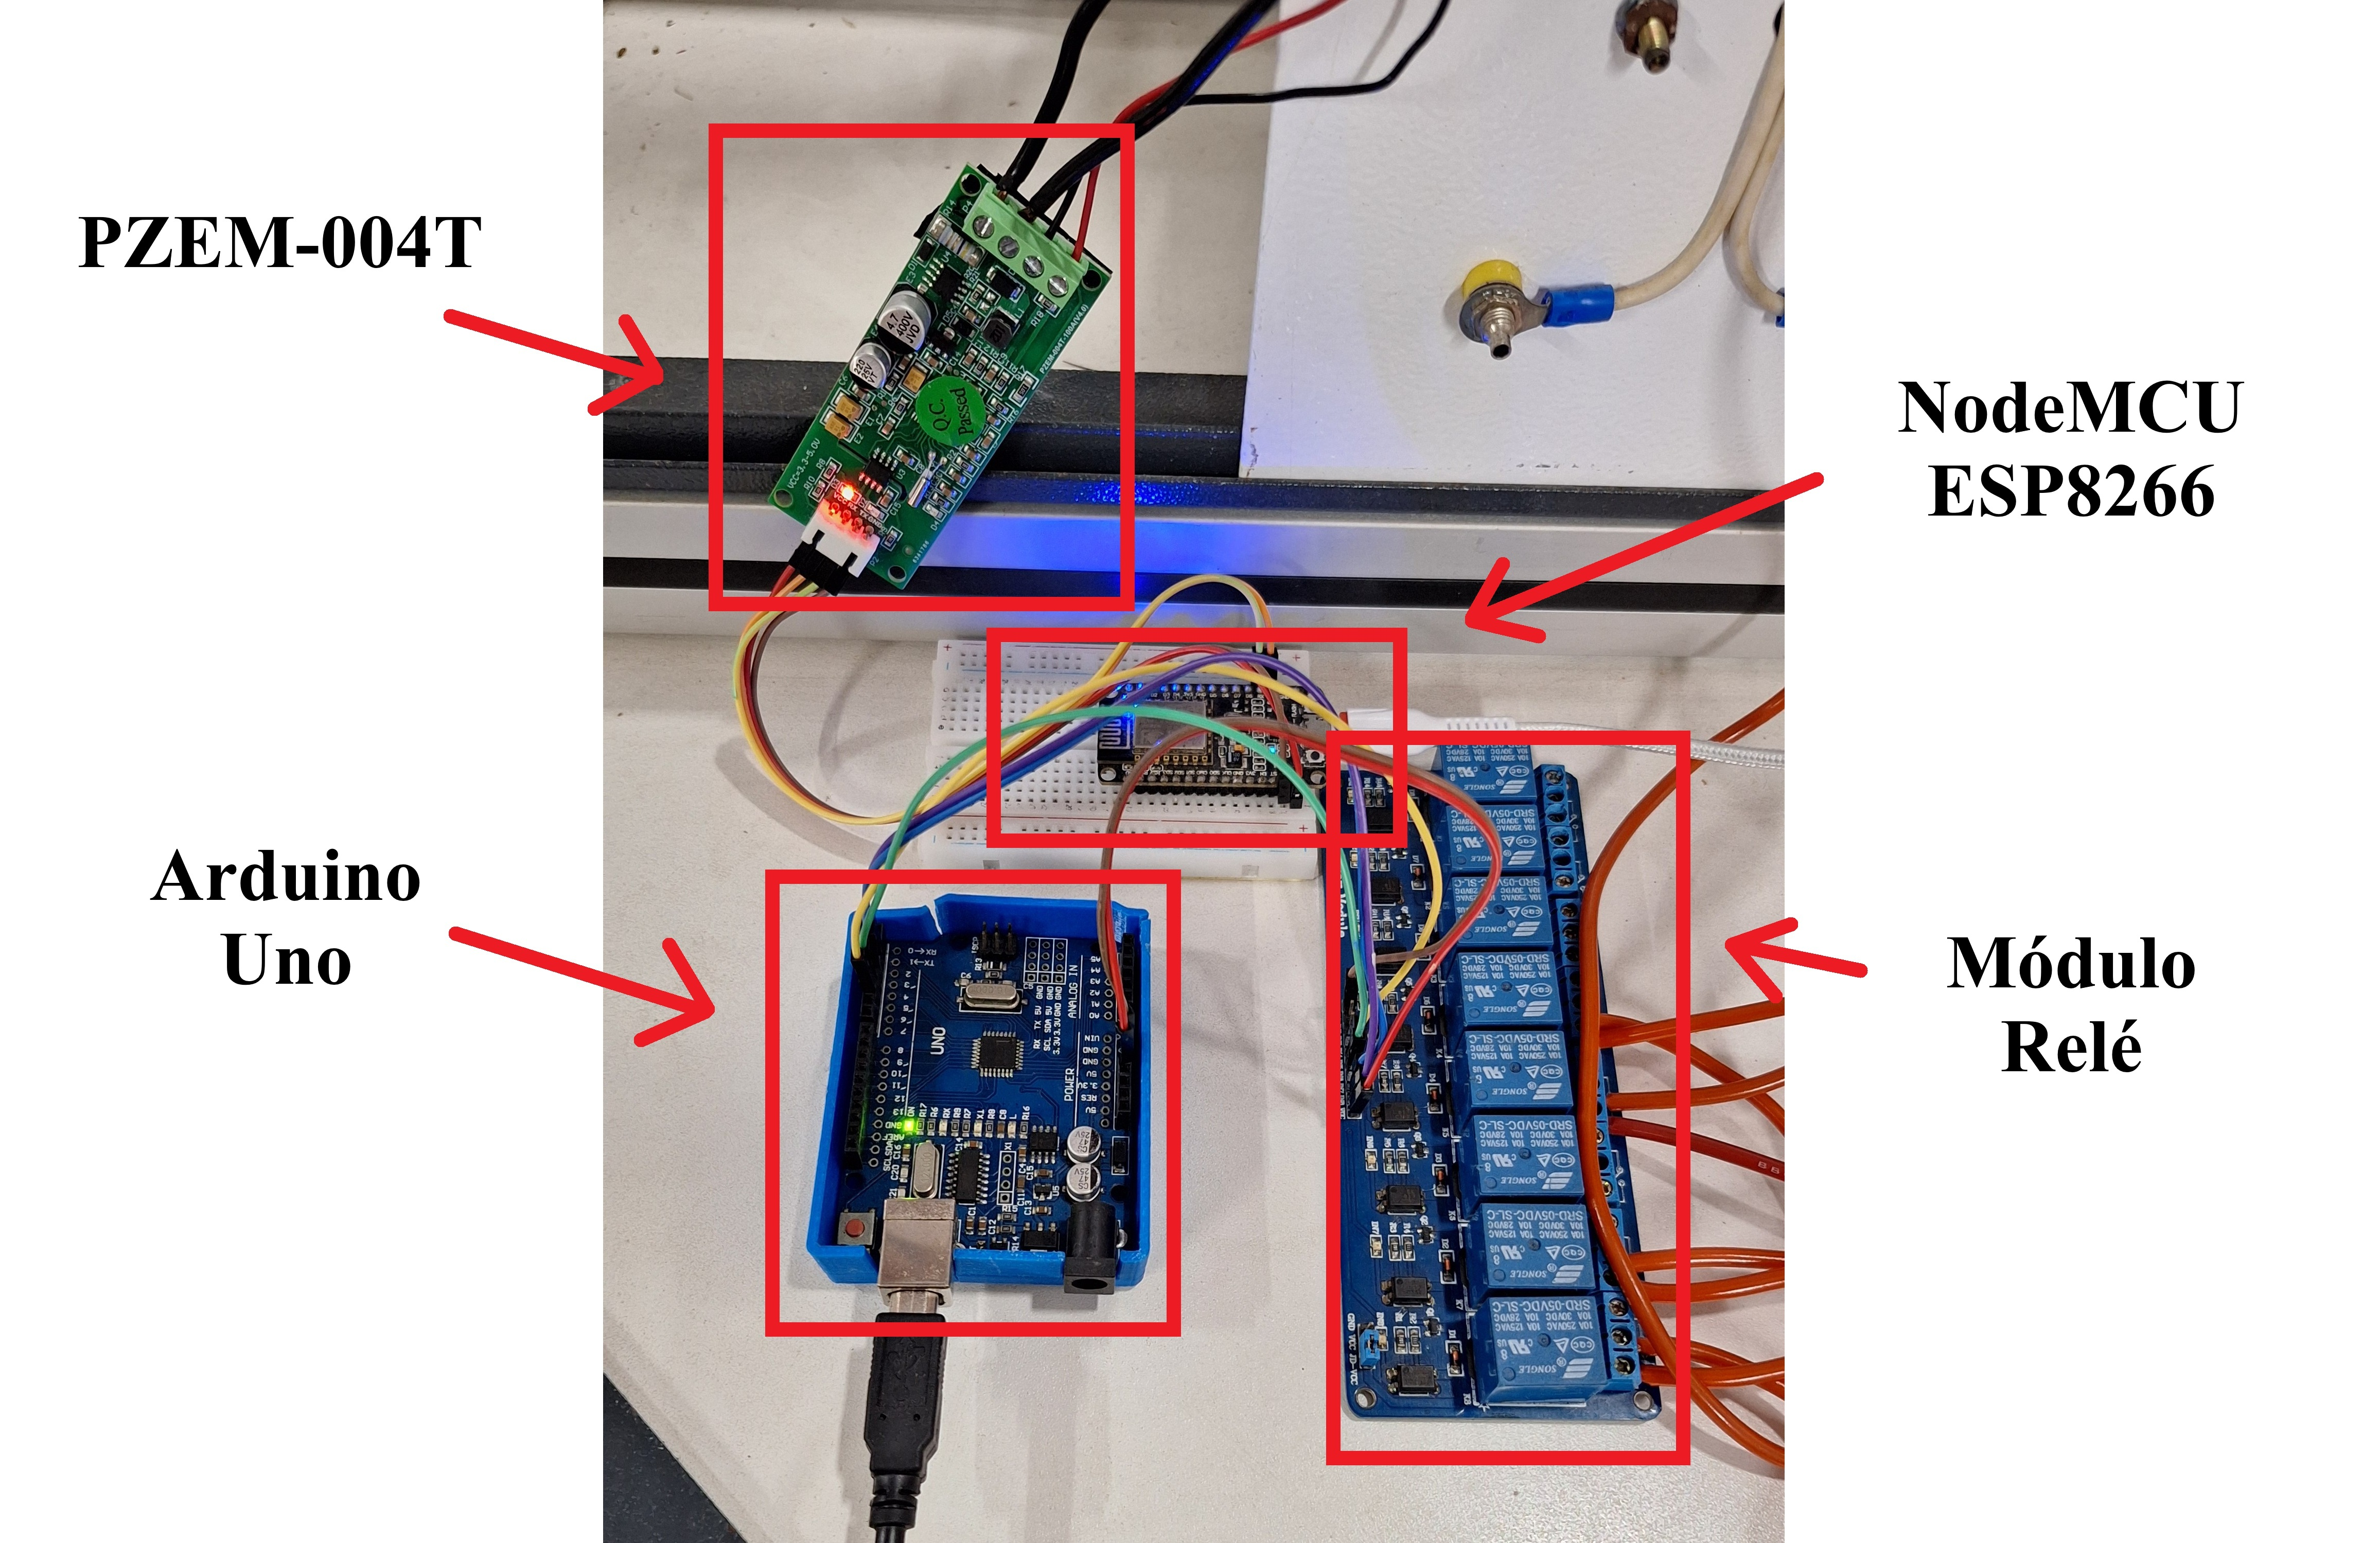
\includegraphics[width=0.7\textwidth]{Figuras/Sistema-pzem-rele-nodemcu.jpg}
    }
    \fonte{\me{2026}}
    \label{fig:sistema_montado}
\end{figure}

Durante os ensaios, as grandezas elétricas foram medidas pelo sensor PZEM-004T e transmitidas em tempo real ao Node-RED, onde foram processadas pelos modelos de aprendizado de máquina. Para validação, as medições do sensor e as estimativas dos modelos foram comparadas com um medidor comercial de referência. 

\begin{table}[!htbp]
    \centering
    \caption{Comparação entre medições do medidor de referência, sensor PZEM-004T e estimativas do modelo.}
    \begin{tabular*}{\textwidth}{@{\extracolsep{\fill}}lccccc@{}}
    \hline
    \textbf{Carga} & \textbf{FP (Ref.)} & \textbf{I (Ref.)} & \textbf{FP (PZEM)} & \textbf{I (PZEM)} & \textbf{FP Est.} \\
    \hline
    Sem carga & 1,00 & 0,00 & 1,00 & 0,00 & 0,29 \\
    Capacitiva & 0,00 & 1,19 & 0,01 & 1,23 & 0,02  \\
    Indutiva & 0,08 & 2,69 & 0,09 & 2,93 & 0,11  \\
    Resistiva & 1,00 & 0,45 & 1,00 & 0,46 & 1,01 \\
    Motor & 0,29 & 2,84 & 0,31 & 2,82 & 0,31 \\
    Resistiva + capacitiva & 0,36 & 1,29 & 0,34 & 1,32 & 0,34 \\
    Resistiva + indutiva & 0,25 & 2,75 & 0,25 & 2,96 & 0,25 \\
    Capacitiva + indutiva & 0,15 & 1,52 & 0,13 & 1,95 & 0,13 \\
    \hline
    \end{tabular*}
    \fonte{\me{2026}}
    \label{tab:validacao_tempo_real}
\end{table}

Conforme Tabela \ref{tab:validacao_tempo_real}, observam-se pequenas diferenças entre as leituras do medidor de referência e aquelas obtidas pelo sensor PZEM. Essas variações podem ser atribuídas à precisão limitada do sensor utilizado e às diferenças de resolução entre os equipamentos de medição, ou ainda, estarem associadas a possíveis imprecisões de calibração do sensor ou a pequenas resistências internas do dispositivo, como por exemplo na situação sem carga, em que o FP estimado foi de 0,29. Ainda assim, os resultados evidenciam que o modelo de regressão foi capaz de reproduzir adequadamente o comportamento das grandezas elétricas do sistema, mesmo diante de pequenas variações nas medições experimentais.

Além disso, o modelo de classificação foi capaz de identificar corretamente o tipo de carga em todos os cenários avaliados, demonstrando a viabilidade do sistema proposto para aplicações de monitoramento inteligente em tempo real.

% \newpage
Os resultados para cada cenário de carga podem ser observados nas Figuras \ref{fig:painel_sem_carga} (sem carga), \ref{fig:painel_capacitiva} (carga capacitiva), \ref{fig:painel_indutiva} (carga indutiva), \ref{fig:painel_resistiva} (carga resistiva), \ref{fig:painel_motor} (motor), \ref{fig:painel_res_cap} (resistiva + capacitiva), \ref{fig:painel_res_ind} (resistiva + indutiva) e \ref{fig:painel_cap_ind} (capacitiva + indutiva). Em cada uma, são exibidas as leituras do sensor PZEM-004T, o fator de potência estimado pelo modelo de regressão e a classe de carga identificada pelo modelo de classificação.

\begin{figure}[h]
    \centering
    \caption{Painel de monitoramento Node-RED para carga sem carga.}
    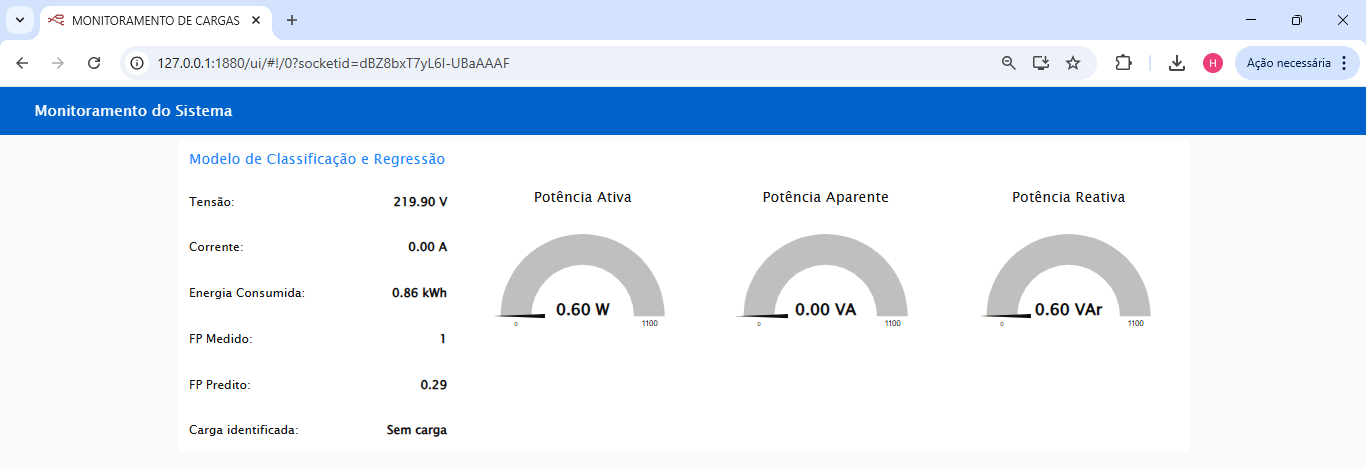
\includegraphics[width=1\textwidth]{Figuras/tela_sem_carga.png}
    \fonte{\me{2026}}
    \label{fig:painel_sem_carga}
\end{figure}

\begin{figure}[h]
    \centering
    \caption{Painel de monitoramento Node-RED para carga capacitiva.}
    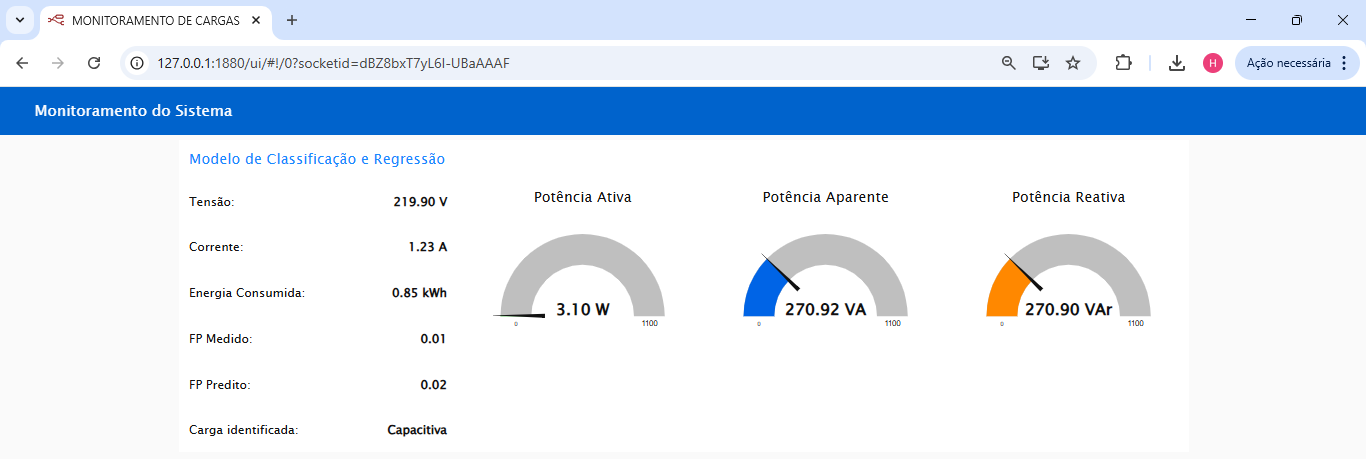
\includegraphics[width=1\textwidth]{Figuras/tela_carga_capacitiva.png}
    \fonte{\me{2026}}
    \label{fig:painel_capacitiva}
\end{figure}

\begin{figure}[h]
    \centering
    \caption{Painel de monitoramento Node-RED para carga indutiva.}
    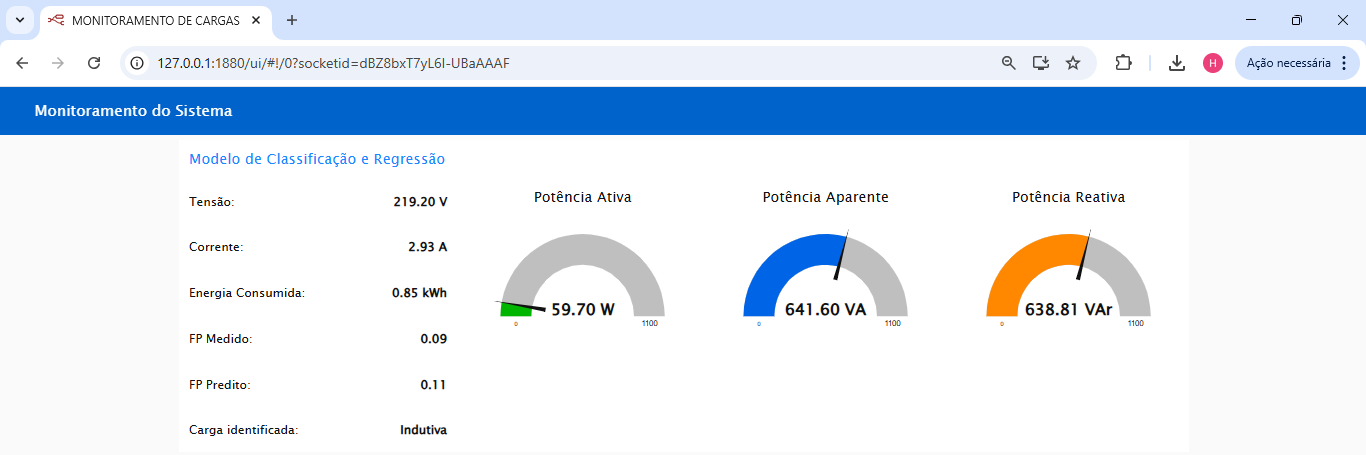
\includegraphics[width=1\textwidth]{Figuras/tela_carga_indutiva.png}
    \fonte{\me{2026}}
    \label{fig:painel_indutiva}
\end{figure}

\begin{figure}[h]
    \centering
    \caption{Painel de monitoramento Node-RED para carga resistiva.}
    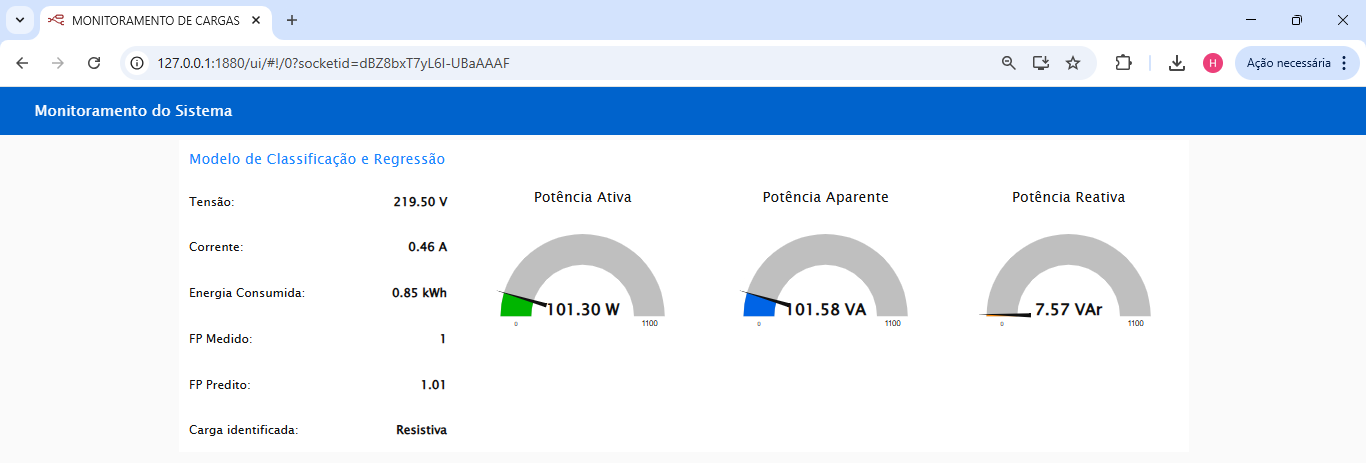
\includegraphics[width=1\textwidth]{Figuras/tela_carga_resistiva.png}
    \fonte{\me{2026}}
    \label{fig:painel_resistiva}
\end{figure}

\begin{figure}[h]
    \centering
    \caption{Painel de monitoramento Node-RED para motor.}
    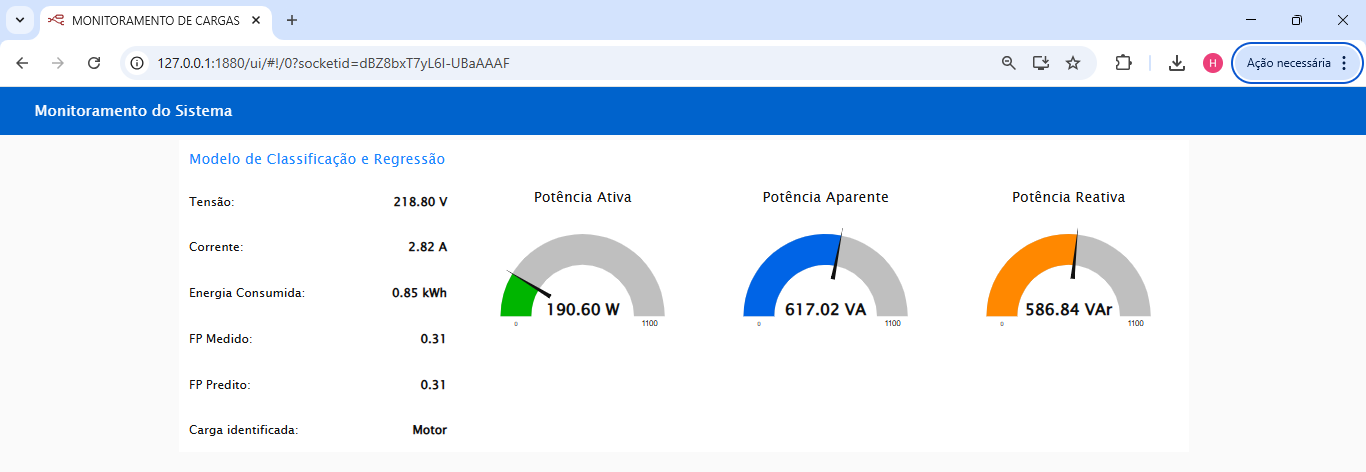
\includegraphics[width=1\textwidth]{Figuras/tela_carga_motor.png}
    \fonte{\me{2026}}
    \label{fig:painel_motor}
\end{figure}

\begin{figure}[h]
    \centering
    \caption{Painel de monitoramento Node-RED para carga resistiva + capacitiva.}
    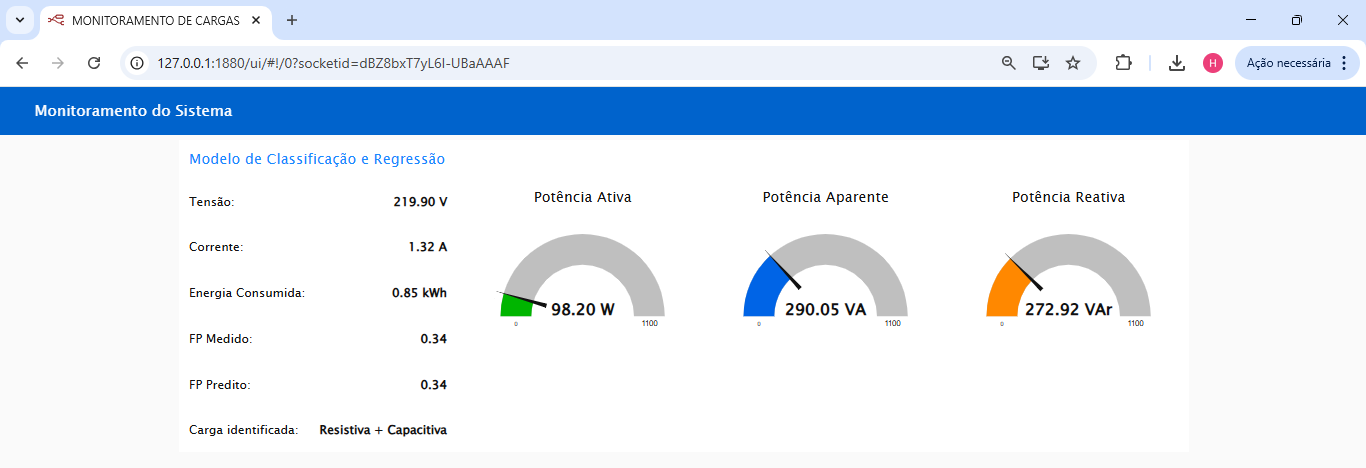
\includegraphics[width=1\textwidth]{Figuras/tela_carga_capacitiva_resisttiva.png}
    \fonte{\me{2026}}
    \label{fig:painel_res_cap}
\end{figure}

\begin{figure}[h]
    \centering
    \caption{Painel de monitoramento Node-RED para carga resistiva + indutiva.}
    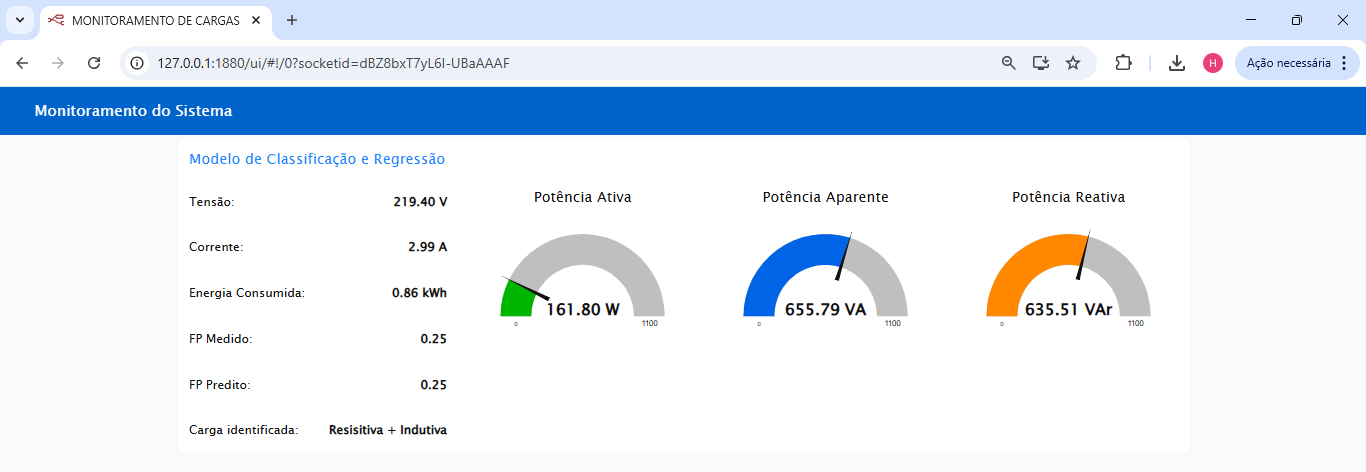
\includegraphics[width=1\textwidth]{Figuras/tela_carga_indutiva_resistiva.png}
    \fonte{\me{2026}}
    \label{fig:painel_res_ind}
\end{figure}

\begin{figure}[h]
    \centering
    \caption{Painel de monitoramento Node-RED para carga capacitiva + indutiva.}
    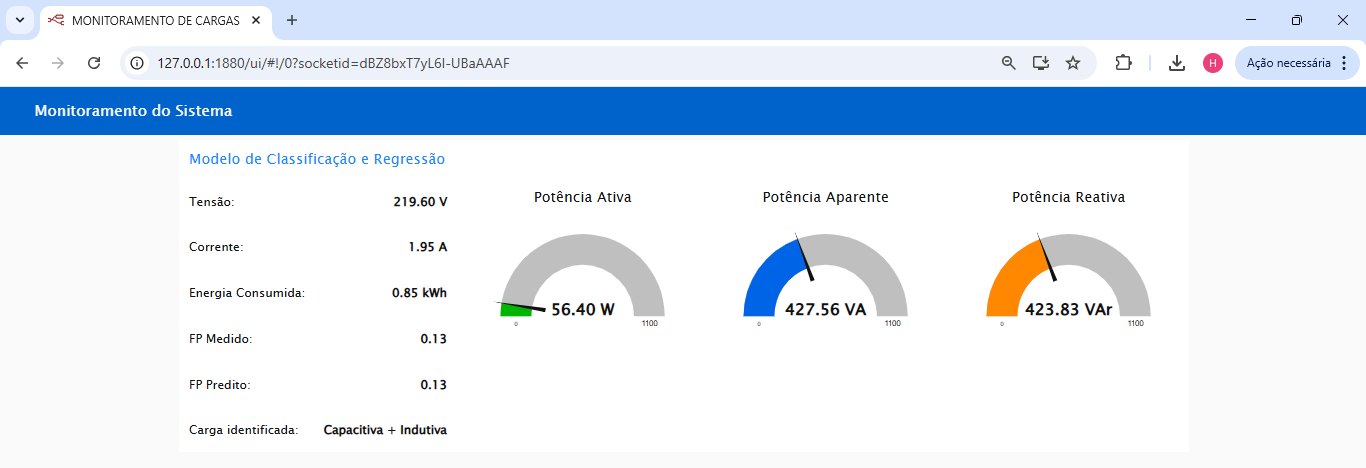
\includegraphics[width=1\textwidth]{Figuras/tela_carga_capacitiva_indutiva.png}
    \fonte{\me{2026}}
    \label{fig:painel_cap_ind}
\end{figure}

\clearpage
Apesar dos bons resultados obtidos, algumas limitações foram identificadas ao longo do desenvolvimento, para fins de considerações em melhorias futuras:
\begin{itemize}
    \item O sensor PZEM-004T apresentou pequenas variações nas medições em comparação com o medidor de referência, especialmente em condições de baixa carga;
    \item A base de dados experimental foi coletada em ambiente laboratorial controlado, podendo não refletir integralmente a complexidade de cenários reais;
    \item Os modelos foram treinados para oito classes de carga específicas (motor de indução, lâmpada incandescente, banco de capacitores de 15 $\mu$F, além de combinações entre eles), limitando sua aplicação a configurações similares e evidenciando a necessidade de expansão do horizonte de cargas;
    \item A estimativa do fator de potência na condição sem carga apresentou desvio devido a características intrínsecas do sensor.
\end{itemize}

% A Figura \ref{fig:painel_monitoramento_nodered} apresenta o painel de monitoramento desenvolvido no Node-RED, com as leituras do PZEM, o fator de potência estimado pelo modelo de regressão e a classe de carga identificada pelo modelo de classificação para cada cenário de carga testado.
% \begin{figure}[h]
%     \centering
%     \caption{Leituras do PZEM exibidas no painel de monitoramento Node-RED.}
    
%     % Linha 1
%     \subfigure[Sem carga]{
%         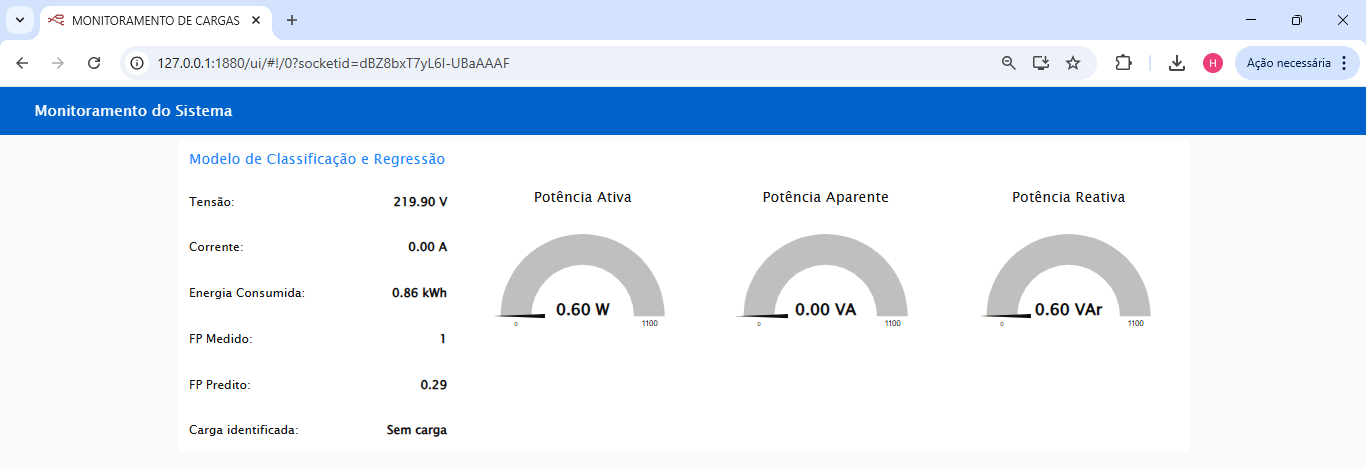
\includegraphics[width=0.48\textwidth]{Figuras/tela_sem_carga.png}
%     }
%     \hfill
%     \subfigure[Capacitiva]{
%         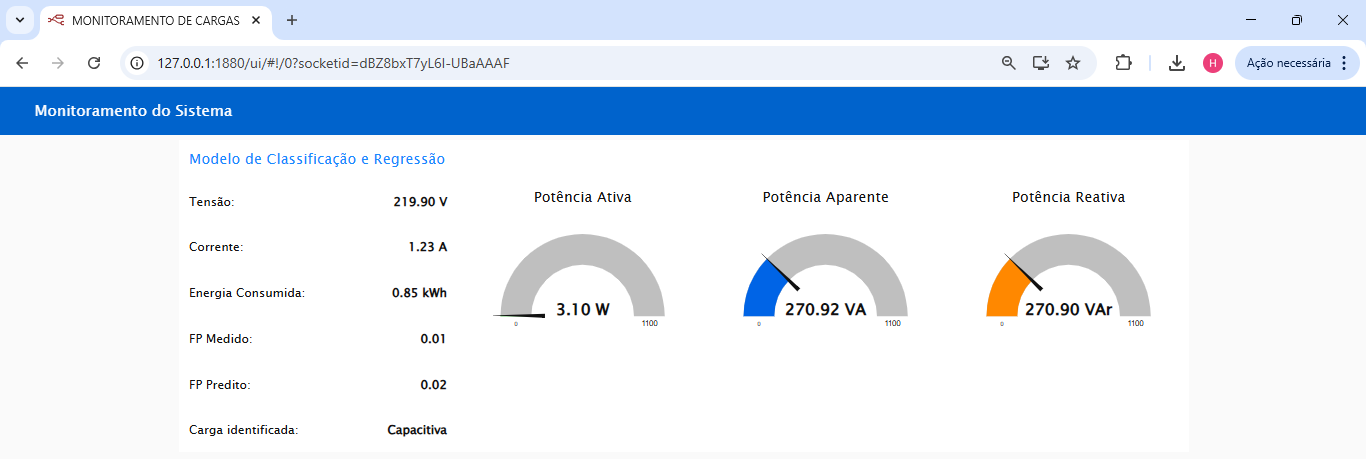
\includegraphics[width=0.48\textwidth]{Figuras/tela_carga_capacitiva.png}
%     }
    
%     \vspace{0.2cm}
    
%     % Linha 2
%     \subfigure[Indutiva]{
%         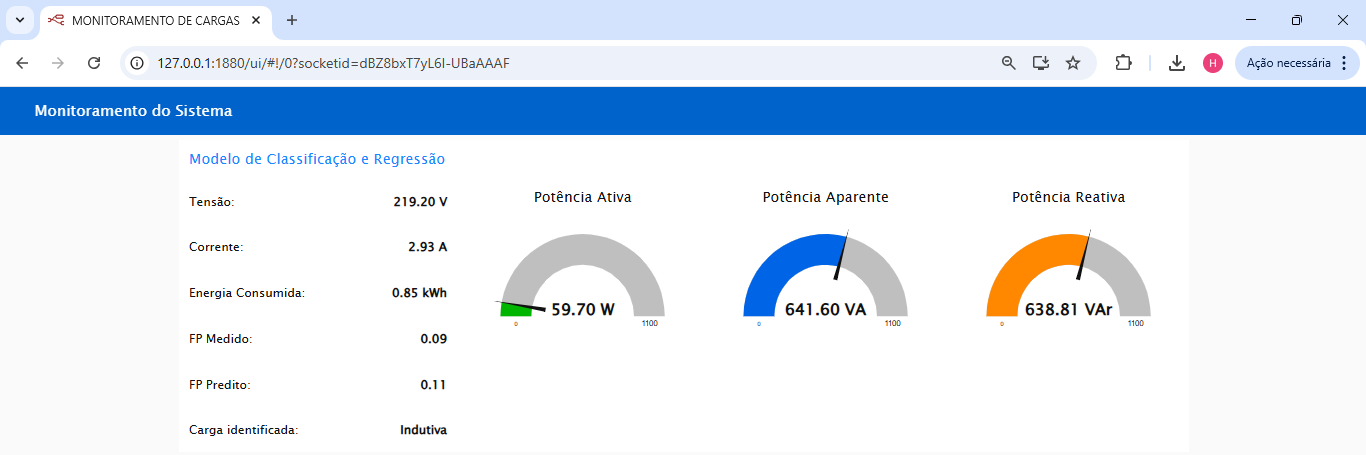
\includegraphics[width=0.48\textwidth]{Figuras/tela_carga_indutiva.png}
%     }
%     \hfill
%     \subfigure[Resistiva]{
%         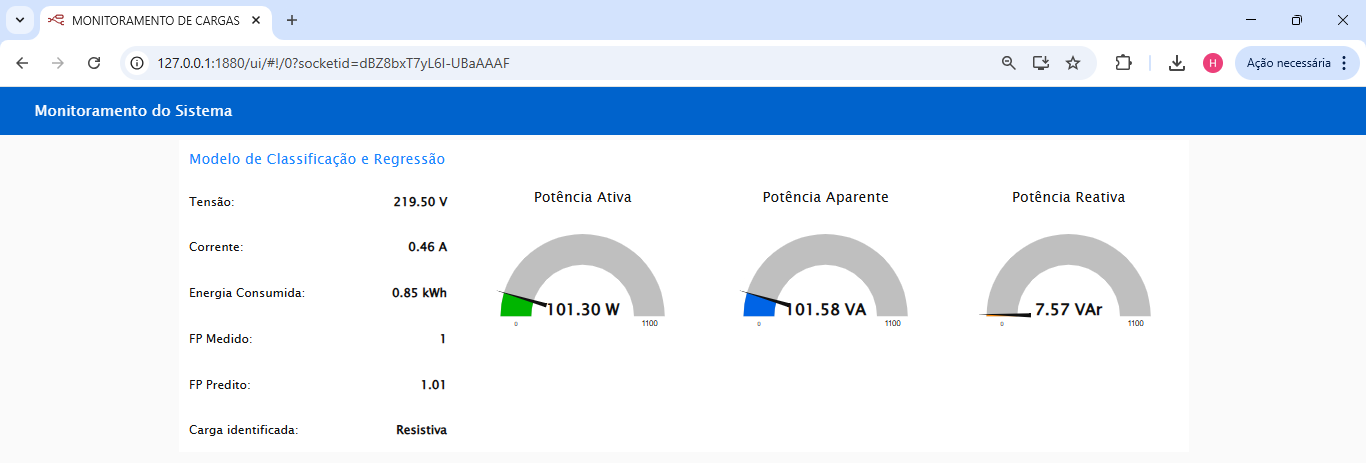
\includegraphics[width=0.48\textwidth]{Figuras/tela_carga_resistiva.png}
%     }
    
%     \vspace{0.2cm}
    
%     % Linha 3
%     \subfigure[Motor]{
%         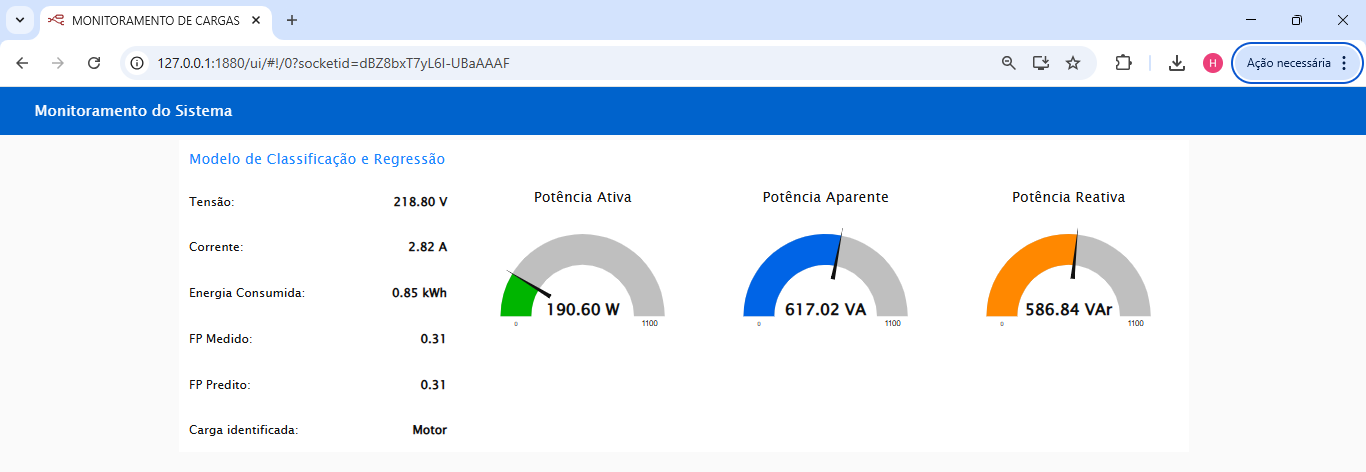
\includegraphics[width=0.48\textwidth]{Figuras/tela_carga_motor.png}
%     }
%     \hfill
%     \subfigure[Resistiva + Capacitiva]{
%         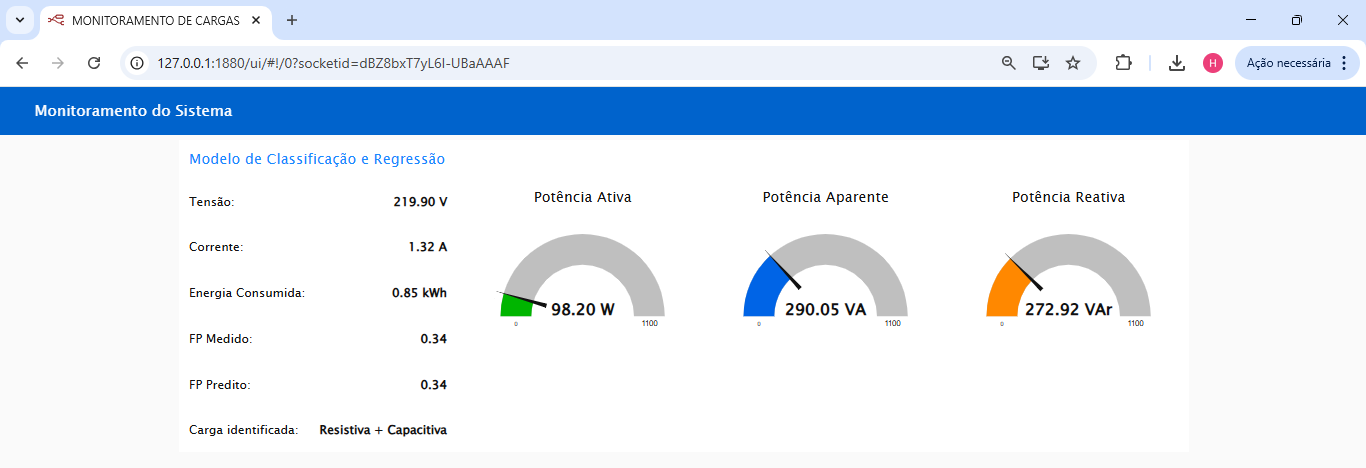
\includegraphics[width=0.48\textwidth]{Figuras/tela_carga_capacitiva_resisttiva.png}
%     }
    
%     \vspace{0.2cm}
    
%     % Linha 4
%     \subfigure[Resistiva + Indutiva]{
%         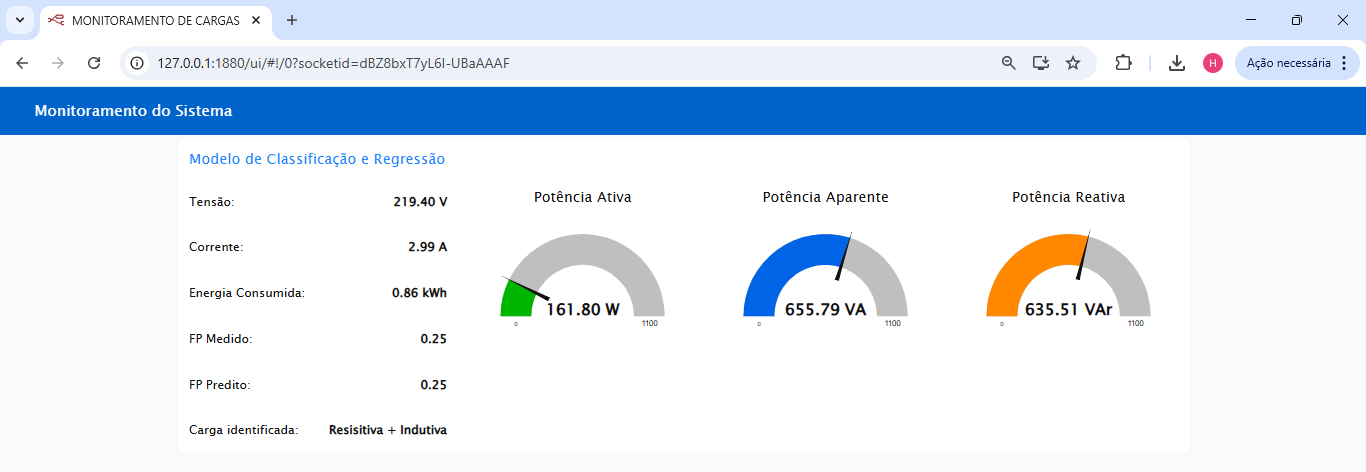
\includegraphics[width=0.48\textwidth]{Figuras/tela_carga_indutiva_resistiva.png}
%     }
%     \hfill
%     \subfigure[Capacitiva + Indutiva]{
%         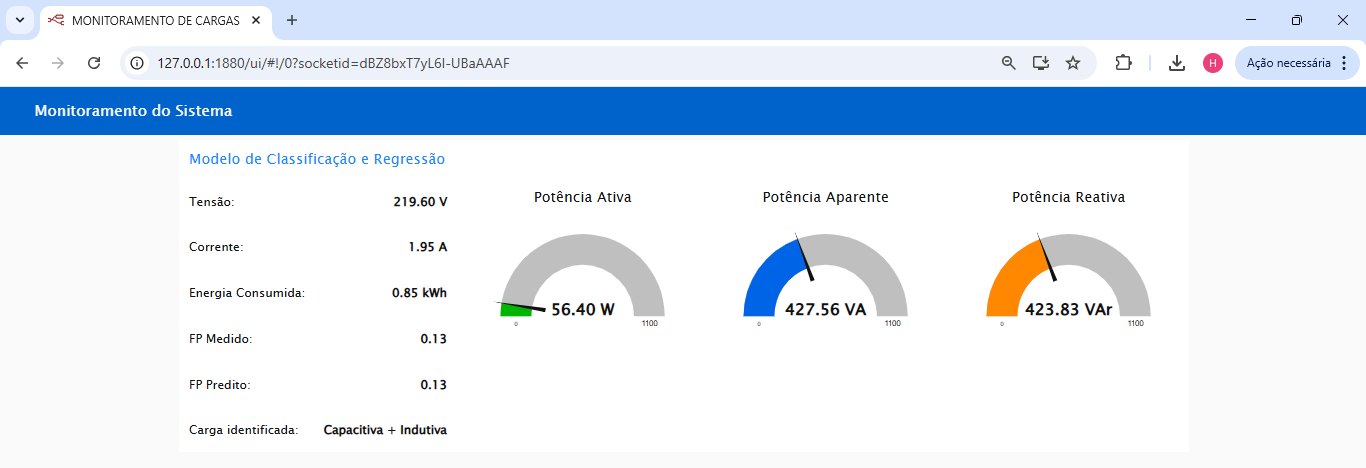
\includegraphics[width=0.48\textwidth]{Figuras/tela_carga_capacitiva_indutiva.png}
%     }
    
%     \fonte{\me{2026}}
%     \label{fig:painel_monitoramento_nodered}
% \end{figure}

% --------------------------------------------------------
% A análise exploratória da base residencial \textit{Individual Household Electric Power Consumption - UCI} teve como finalidade compreender o comportamento das grandezas elétricas e sua relação com o fator de potência (FP), com o objetivo de selecionar as variáveis de maior relevância para o treinamento dos modelos. 

% A base contempla medições realizadas entre os anos de 2006 e 2010, porém, para este estudo, foi selecionado um recorte correspondente a um ano completo de dados referente a 2010. O código desenvolvido e o acesso à base de dados dessa análise estão disponíveis no Apêndice \ref{apendice_análise_UCI}.

% Inicialmente, foi realizada uma análise da sazonalidade mensal do fator de potência médio, conforme ilustrado na Figura \ref{fig:fp_sazonalidade}. Os resultados permitem observar variações significativas ao longo do ano, indicando que o fator de potência sofre influência direta das mudanças no perfil de consumo e da combinação de cargas presentes no sistema elétrico ao longo das estações.

% \begin{figure}[!htbp] 
%     \centering
%     \caption{Análise de sazonalidade mensal do fator de potência.} 
%     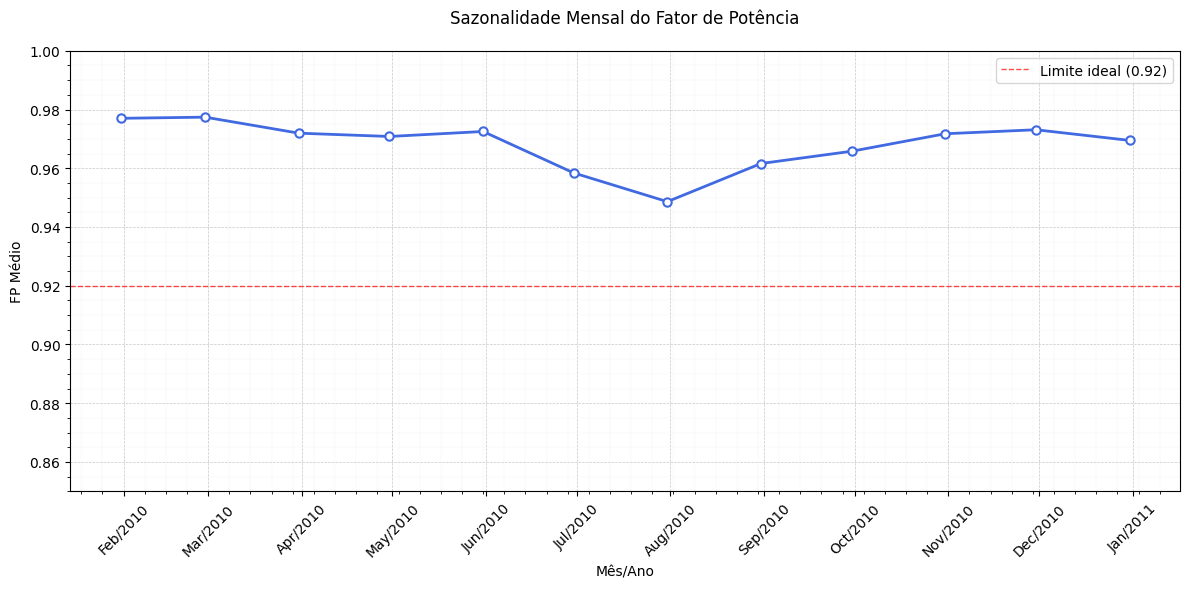
\includegraphics[width = 1\textwidth]{Figuras/sazonalidade mesal do fp.png} 
%     \fonte{\me{2026}} 
%     \label{fig:fp_sazonalidade} 
% \end{figure}

% Posteriormente, foi realizada a avaliação da correlação entre o fator de potência e as principais grandezas elétricas disponíveis na base de dados, incluindo potência ativa média global, potência reativa, tensão e intensidade de corrente média global. A matriz de correlação apresentada na Figura \ref{fig:correlacao_variaveis} mostra que o FP tem correlação negativa mais expressiva com a potência reativa ($r \approx -0{,}47$) e positiva fraca com potência ativa ($r \approx 0{,}40$). Embora as correlações entre o fator de potência, corrente e potência aparente sejam moderadas ($r \approx 0{,}38$), a corrente apresenta forte correlação com a potência ativa ($r \approx 1$) e com a potência aparente ($r \approx 1$), evidenciando a relação esperada entre essas grandezas. Por outro lado, a tensão apresentou correlação com o fator de potência praticamente nula ($r \approx 0{,}13$), o que indica que essa grandeza, isoladamente, não é um bom preditor do FP. Por esse motivo, não foi incluída como variável de entrada no treinamento dos modelos.

% \begin{figure}[!htbp] 
%     \centering
%     \caption{Matriz de correlação das variáveis elétricas.} 
%     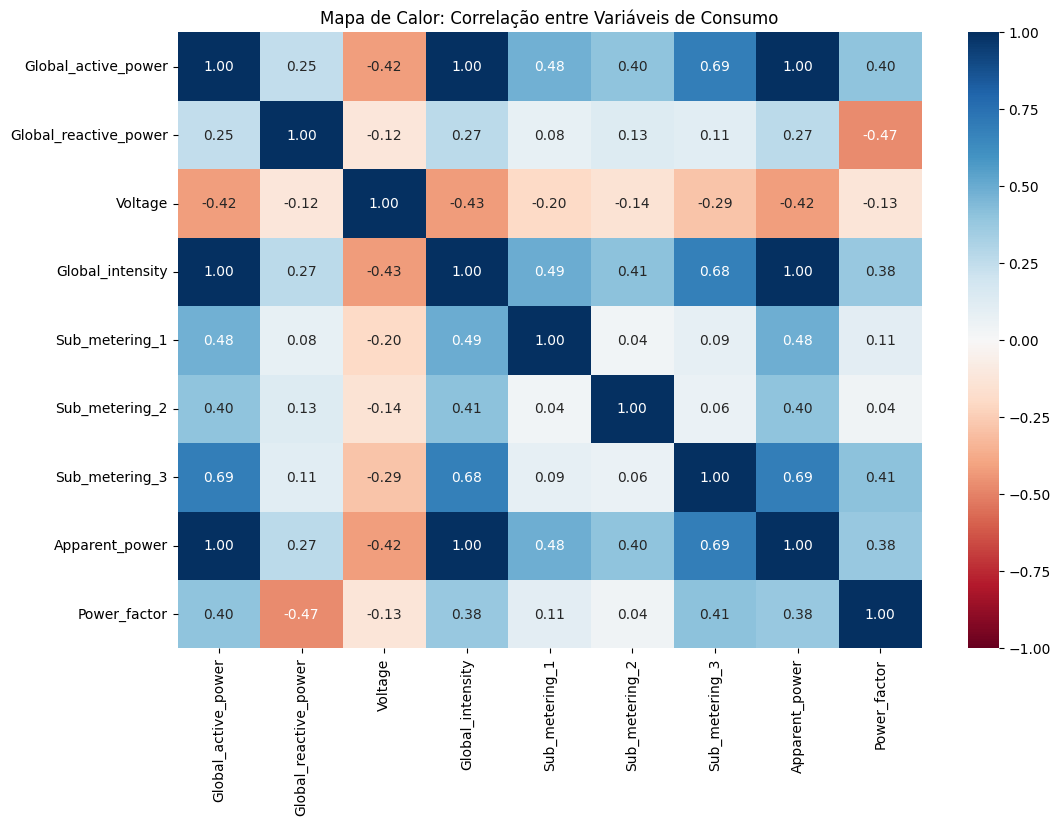
\includegraphics[width = 1\textwidth]{Figuras/mapa de correlação.png} 
%     \fonte{\me{2026}} 
%     \label{fig:correlacao_variaveis} 
% \end{figure}

% A análise evidenciou que o fator de potência apresenta relação significativa com as variáveis associadas às potências ativa, reativa, aparente e intensidade de corrente, conforme detalhado na Figura \ref{fig:graficos_relacao_fp}. Tal comportamento é esperado do ponto de vista físico, uma vez que o fator de potência está diretamente relacionado à relação entre potência ativa e aparente em sistemas elétricos, conforme Equação \eqref{eq:fp}. Dessa forma, variações nas potências e na corrente de consumo impactam diretamente o valor do fator de potência observado.

% Além disso, foram investigados os períodos de ocorrência dos menores valores de fator de potência ao longo da série temporal, buscando identificar possíveis padrões associados a mudanças no perfil de consumo. Para essa análise, foram considerados os 1\% menores valores de fator de potência da base de dados, correspondendo a valores iguais ou inferiores a 0,8057. Nesse subconjunto, observou-se um valor médio de 0,7829, com mínimo de 0,6175 e máximo de 0,8057, conforme Figura \ref{fig:resumo_estatistico_menores_FP}, caracterizando as condições mais críticas de operação em termos de fator de potência.

% \begin{figure}[!htbp] 
%     \centering
%     \caption{Resumo estatístico dos menores FPs.} 
%     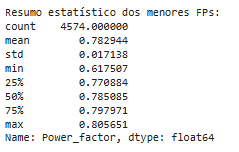
\includegraphics{Figuras/Resumo estatístico dos menores FPs.png} 
%     \fonte{\me{2026}} 
%     \label{fig:resumo_estatistico_menores_FP} 
% \end{figure}

% A distribuição temporal dessas ocorrências revelou um padrão horário bem definido. Conforme ilustrado na Figura \ref{fig:distribuicao_menores_fp}, a maior concentração de valores críticos ocorre durante o período da madrugada, com pico de ocorrências às 4h (377 registros). Esse comportamento sugere que os menores valores de fator de potência tendem a ocorrer em períodos de menor demanda elétrica global, quando a participação relativa de cargas com características reativas se torna mais significativa. Esse padrão pode estar associado ao funcionamento de determinados equipamentos operando em regime contínuo durante a madrugada, como motores de pequena potência e sistemas de refrigeração.

% \begin{figure}[!htbp] 
%     \centering
%     \caption{Distribuição horária das ocorrências dos menores valores de fator de potência.} 
%     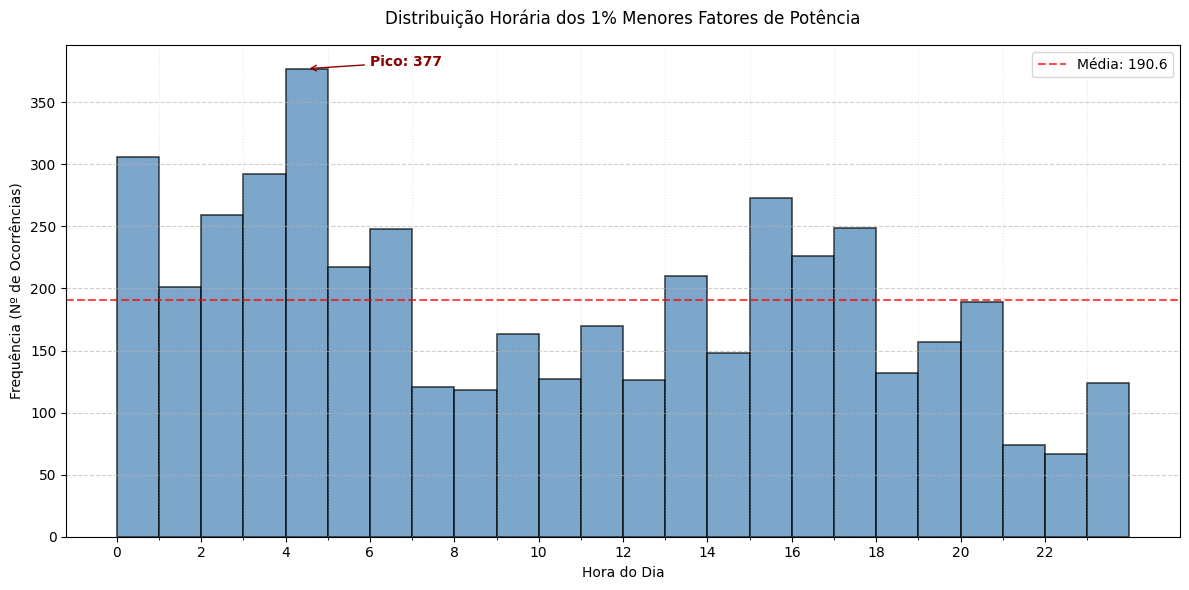
\includegraphics[width=1\textwidth]{Figuras/distribuicao menores fp.png} 
%     \fonte{\me{2026}} 
%     \label{fig:distribuicao_menores_fp} 
% \end{figure} 

% \begin{figure}[h]
%     \centering
%     \caption{Relações entre grandezas elétricas e o fator de potência}
%     \subfigure[Relação P x FP.]{
%         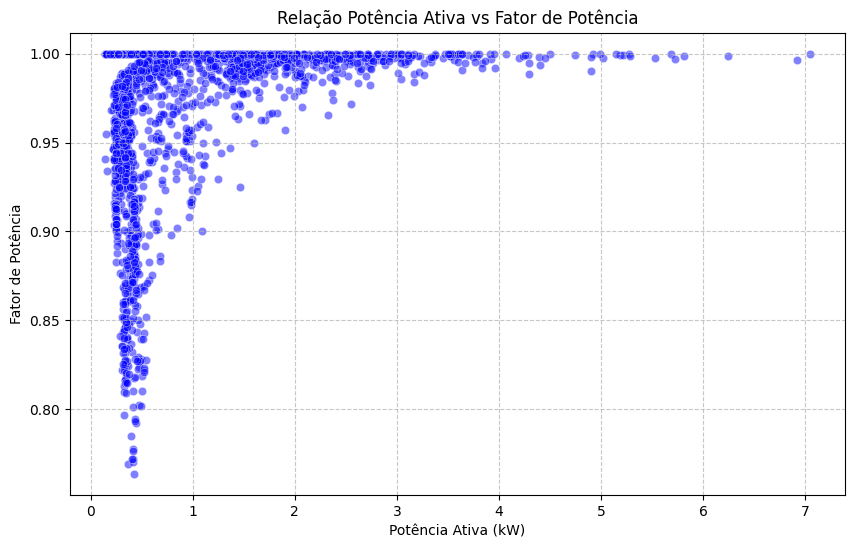
\includegraphics[width=0.75\textwidth]{Figuras/grafico de relação P VS fp.png}
%     }
%     \hfill % Adiciona espaço entre as imagens
%     \subfigure[Relação Q x FP.]{
%         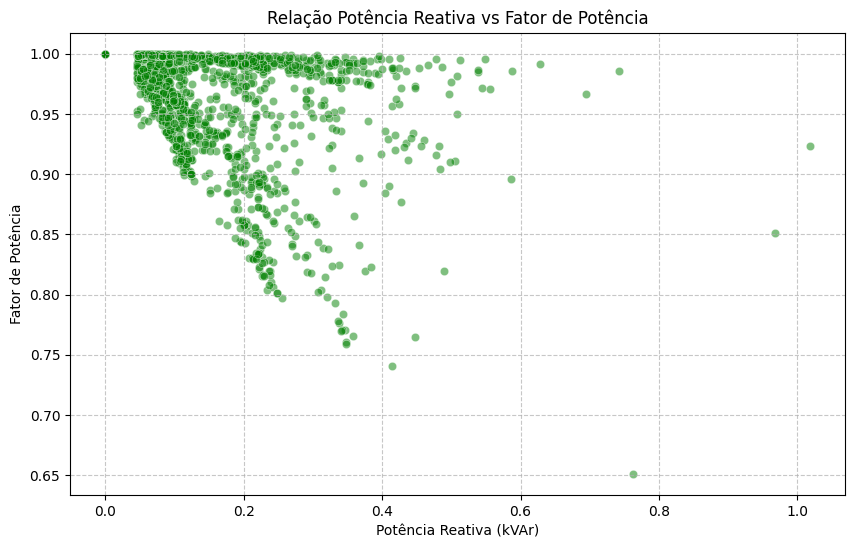
\includegraphics[width=0.75\textwidth]{Figuras/grafico de relação Q VS fp.png}
%     }
%     \hfill
%     \subfigure[Relação I x FP.]{
%         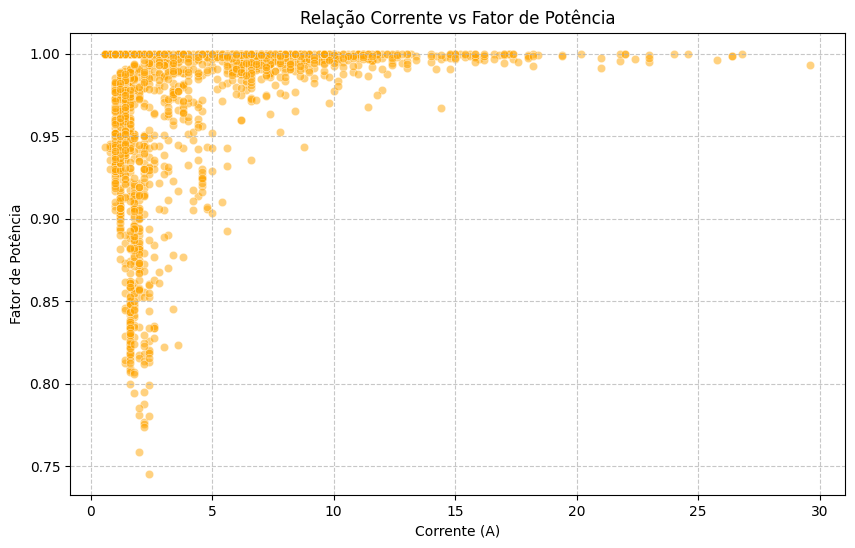
\includegraphics[width=0.75\textwidth]{Figuras/grafico de relação I VS fp.png}
%     }
%     \fonte{\me{2026}} 
%     \label{fig:graficos_relacao_fp}
% \end{figure}
    % Resultados e Discussão
 \chapter{Conclusão} \label{Conclusão}

Este trabalho apresentou o desenvolvimento de um sistema inteligente de monitoramento elétrico em tempo real, integrando sensoriamento de baixo custo, comunicação IoT e modelos de aprendizado de máquina para classificação de cargas e estimativa do fator de potência. A solução proposta foi implementada utilizando o sensor PZEM-004T para aquisição das grandezas elétricas, o microcontrolador NodeMCU ESP8266 para transmissão dos dados via protocolo MQTT e a plataforma Node-RED para processamento e visualização em tempo real.

Os modelos de aprendizado de máquina, baseados na arquitetura Multilayer Perceptron (MLP), foram treinados na plataforma Edge Impulse a partir de uma base de dados experimental contendo 1000 amostras para cada uma das oito classes de carga consideradas. O modelo de classificação alcançou acurácia de 100\%, com valores de precisão, recall e F1-score iguais a 1,0 para todas as classes, demonstrando excelente capacidade de distinção entre os diferentes tipos de carga. O modelo de regressão apresentou erro quadrático médio de \(8,30 \times 10^{-6}\) e erro absoluto médio de 0,00228 no conjunto de teste, com coeficiente de variância explicada de 0,9997, evidenciando elevada precisão na estimativa do fator de potência.

A validação experimental em bancada confirmou a eficácia do sistema, com o modelo de classificação identificando corretamente o tipo de carga em todos os cenários avaliados e o modelo de regressão apresentando estimativas consistentes com as medições do sensor. A integração com a plataforma Node-RED permitiu o desenvolvimento de um painel de monitoramento intuitivo, possibilitando a visualização em tempo real das grandezas elétricas, da classe de carga identificada e do fator de potência estimado.

Os resultados obtidos demonstram que é viável desenvolver sistemas de monitoramento inteligente de baixo custo combinando tecnologias acessíveis como o PZEM-004T, NodeMCU ESP8266, Node-RED e modelos de aprendizado de máquina. A solução proposta apresenta potencial para melhorias e expansão visando a aplicação em ambientes residenciais, comerciais e/ou industriais, contribuindo para a eficiência energética, a redução de custos operacionais e a prevenção de penalidades regulatórias associadas ao baixo fator de potência.

\section{Trabalhos Futuros}
A partir dos resultados obtidos, destacam-se as seguintes oportunidades para continuidade e aprimoramento da pesquisa:

\begin{itemize}
    \item \textbf{Ampliação da base de dados}: expandir o conjunto de amostras para incluir um número maior de configurações de carga e diferentes condições operacionais, aumentando a representatividade e a robustez dos modelos;

    \item \textbf{Combinações mais complexas de cargas}: explorar cenários com múltiplas cargas operando simultaneamente em diferentes combinações, aproximando o sistema das condições reais de operação em instalações elétricas;

    \item \textbf{Avaliação de técnicas mais sofisticadas}: investigar o desempenho de arquiteturas mais avançadas, como redes neurais recorrentes (RNNs) ou redes de memória de longo prazo (LSTM), para capturar dependências temporais mais complexas;

    \item \textbf{Aplicação de TinyML e Edge AI}: implementar os modelos diretamente no microcontrolador utilizando técnicas de TinyML, eliminando a dependência de processamento externo e viabilizando a execução em sistemas com recursos limitados de memória e energia;

    \item \textbf{Integração com sistemas de gerenciamento energético}: o modelo de classificação pode ser empregado para identificação automática do perfil de consumo, permitindo ações corretivas como o acionamento seletivo de bancos de capacitores;

    \item \textbf{Tomada de decisão automatizada}: a classificação em tempo real viabiliza sistemas inteligentes que ajustam automaticamente a operação de equipamentos com base no tipo de carga identificada;

    \item \textbf{Monitoramento preditivo}: a combinação entre classificação de cargas e estimativa do fator de potência pode subsidiar a detecção precoce de falhas e o planejamento de manutenções preventivas;

    % \item \textbf{Otimização para sistemas embarcados}: explorar técnicas de quantização, poda e compressão de modelos para reduzir o consumo de memória e energia, permitindo a execução eficiente em dispositivos de borda;

    \item \textbf{Validação em cenários reais}: testar o sistema em instalações elétricas reais por períodos prolongados, avaliando seu desempenho sob condições variáveis de operação e carga;

    % \item \textbf{Integração com sistemas de correção automática}: acoplar o sistema de monitoramento a dispositivos de compensação de potência reativa, permitindo a correção automática do fator de potência em tempo real.
\end{itemize}    % Conclusão

% ---------------------------------------------------------------
% ELEMENTOS PÓS-TEXTUAIS
% ---------------------------------------------------------------
\postextual

\bibliography{Referencias}	% Referências bibliográficas - Elemento Obrigatório
%\include{PosTextuais/Glossario}				% Elemento Opcional
% ----------------------------------------------------------
% Apêndices
% ----------------------------------------------------------
\begin{apendicesenv}

% Imprime uma página indicando o início dos apêndices
% \partapendices

% Configuração global de estilo para todos os códigos
\definecolor{codered}{RGB}{221,0,0}
\definecolor{codegreen}{RGB}{0,170,0}
\definecolor{codebrown}{RGB}{146,73,0}
\definecolor{codeorange}{RGB}{255,119,0}
\definecolor{backcolour}{RGB}{255,255,255}

\lstdefinestyle{mystyle}{
    backgroundcolor=\color{backcolour},   
    commentstyle=\color{codered},
    keywordstyle=\color{codeorange},
    numberstyle=\tiny\color{codebrown},
    stringstyle=\color{codegreen},
    basicstyle=\ttfamily\footnotesize,
    breakatwhitespace=false,         
    breaklines=true,                 
    captionpos=b,                    
    keepspaces=true,                 
    numbers=left,                    
    numbersep=5pt,                  
    showspaces=false,                
    showstringspaces=false,
    showtabs=false,                  
    tabsize=2,
    frame=single,
    frameround=tttt,
    rulecolor=\color{black!30},
    aboveskip=20pt,
    belowskip=20pt
}

\lstset{style=mystyle}

% Configuração para acentuação
\lstset{literate=
    {á}{{\'a}}1 {à}{{\`a}}1 {ã}{{\~a}}1 {â}{{\^a}}1
    {é}{{\'e}}1 {ê}{{\^e}}1 {í}{{\'i}}1 {ó}{{\'o}}1
    {õ}{{\~o}}1 {ô}{{\^o}}1 {ú}{{\'u}}1 {ü}{{\"u}}1
    {ç}{{\c{c}}}1 {Á}{{\'A}}1 {À}{{\`A}}1 {Ã}{{\~A}}1
    {Â}{{\^A}}1 {É}{{\'E}}1 {Ê}{{\^E}}1 {Í}{{\'I}}1
    {Ó}{{\'O}}1 {Õ}{{\~O}}1 {Ú}{{\'U}}1 {Ç}{{\c{C}}}1
    {_}{{\_}}1
}

% ----------------------------------------------------------
% ----------------------------------------------------------
% ----------------------------------------------------------
% APÊNDICE A - Código Arduino para Coleta de Dados
% ----------------------------------------------------------
\chapter{Código de coleta dos dados do sensor PZEM}
\label{apendice_coleta_dados}

Código implementado EM C++ para leitura e coleta das grandezas medidas pelo sensor PZEM via monitor serial.

\begin{lstlisting}[language=C++, caption={Coleta dos dados do sensor PZEM.}, label=cod_controle_manual]
/*
===================================================================
Autor: Hirislayne Batista Ramos dos Santos

COLETA DE DADOS PZEM004T - ARDUINO UNO 
Coleta 1000 amostras a 1 segundo
Sem acionamento de relés - Controle de cargas externamente
===================================================================
*/

#include <PZEM004Tv30.h>
#include <SoftwareSerial.h>

#define TOTAL_AMOSTRAS 1000      // 1000 amostras no total
#define INTERVALO_AMOSTRA 1000   // 1 amostra por segundo

// ===== PINOS DO PZEM =====
#define PZEM_RX_PIN 11
#define PZEM_TX_PIN 12
SoftwareSerial pzemSWSerial(PZEM_RX_PIN, PZEM_TX_PIN);
PZEM004Tv30 pzem(pzemSWSerial);

int numAmostras = 0;
unsigned long ultimaAmostra = 0;
bool coletaConcluida = false;

// Variável para identificar a carga manualmente
int cargaAtual = 5;  // Mudar este valor manualmente no código antes de cada coleta

void setup() {
  Serial.begin(115200);
  
  Serial.println(F("=========================================="));
  Serial.println(F("COLETA DE DADOS - PZEM004T"));
  Serial.println(F("=========================================="));
  Serial.print(F("Total de amostras: "));
  Serial.println(TOTAL_AMOSTRAS);
  Serial.print(F("Intervalo: 1 segundo\n"));
  Serial.println(F("IMPORTANTE: Altere a variável 'cargaAtual' no código"));
  Serial.println(F("para identificar qual carga está sendo testada:"));
  Serial.println(F("  0 = SEM CARGA"));
  Serial.println(F("  1 = CAPACITIVA"));
  Serial.println(F("  2 = INDUTIVA"));
  Serial.println(F("  3 = RESISTIVA"));
  Serial.println(F("  4 = MOTOR"));
  Serial.println(F("  5 = CAPACITIVA + RESISTIVA"));
  Serial.println(F("  6 = INDUTIVA + RESISTIVA"));
  Serial.println(F("  7 = CAPACITIVA + INDUTIVA"));
  Serial.println(F("=========================================="));
  
  // Cabeçalho CSV
  Serial.println(F("Carga,Tensao(V),Corrente(A),Potencia_Ativa(W),Potencia_Aparente(VA),Potencia_Reativa(VAR),Fator_Potencia,Energia(kWh),Frequencia(Hz)"));
  
  ultimaAmostra = millis();
}

void loop() {
  // Verifica se a coleta já foi concluída
  if (coletaConcluida) {
    Serial.println(F("=== COLETA CONCLUIDA ==="));
    Serial.print(F("Total de "));
    Serial.print(TOTAL_AMOSTRAS);
    Serial.println(F(" amostras coletadas."));
    while(1);  // Para aqui
  }
  
  // Verifica se é hora de nova amostra
  if (millis() - ultimaAmostra >= INTERVALO_AMOSTRA) {
    
    // Leitura do PZEM
    float V = pzem.voltage();
    float I = pzem.current();
    float P = pzem.power();
    float E = pzem.energy();
    float F = pzem.frequency();
    float FP = pzem.pf();
    
    // Verifica se as leituras são válidas
    if (!isnan(V) && !isnan(I) && !isnan(P) && !isnan(E) && !isnan(F) && !isnan(FP)) {
      
      // Cálculos das potências
      float S = V * I;  // Potência Aparente
      float Q = sqrt(abs(S*S - P*P));  // Potência Reativa
      if (FP < 0) Q = -Q;  // Ajuste de sinal (capacitivo/indutivo)
      
      // ENVIA A AMOSTRA (formato CSV)
      Serial.print(cargaAtual); Serial.print(",");
      Serial.print(V); Serial.print(",");
      Serial.print(I); Serial.print(",");
      Serial.print(P); Serial.print(",");
      Serial.print(S); Serial.print(",");
      Serial.print(Q); Serial.print(",");
      Serial.print(FP); Serial.print(",");
      Serial.print(E); Serial.print(",");
      Serial.println(F);
      
      numAmostras++;
      
      // Verifica se completou
      if (numAmostras >= TOTAL_AMOSTRAS) {
        coletaConcluida = true;
      }
    } else {
      Serial.println(F("ERRO: Leitura inválida do PZEM"));
    }
    
    ultimaAmostra = millis();
  }
}
\end{lstlisting}

% ----------------------------------------------------------
% ----------------------------------------------------------
% APÊNDICE B - Código para Controle dos Relés
% ----------------------------------------------------------
\chapter{Código controle Manual dos Relés via Monitor Serial}
\label{apendice_controle_cargas}

Código implementado em C++ para acionamento manual dos relés das cargas elétricas por meio de comandos enviados via monitor serial.

\begin{lstlisting}[language=C++, caption={Controle manual dos relés das cargas.}, label=cod_controle_manual]
/*
===================================================================
Autor: Hirislayne Batista Ramos dos Santos

COMANDOS:
- 1: Liga relé 2 (Carga Capacitiva)
- q: Desliga relé 2
- 2: Liga relé 3 (Carga Indutiva)
- w: Desliga relé 3
- 3: Liga relé 4 (Lâmpada)
- e: Desliga relé 4
- 4: Liga relé 5 (Motor)
- r: Desliga relé 5
- a: Liga todos os relés
- s: Desliga todos os relés
- h: Mostra esta ajuda
===================================================================
*/

// Definição dos pinos dos relés
const int rele_capacitiva = 2;
const int rele_indutiva = 3;
const int rele_resistiva = 4;
const int rele_motor = 5;

void setup() {
  Serial.begin(115200);
  
  // Configura todos os pinos como saída
  pinMode(rele_capacitiva, OUTPUT);
  pinMode(rele_indutiva, OUTPUT);
  pinMode(rele_resistiva, OUTPUT);
  pinMode(rele_motor, OUTPUT);
  
  // Garante que todos começam desligados (HIGH = desligado para relé de estado sólido)
  digitalWrite(rele_capacitiva, HIGH);
  digitalWrite(rele_indutiva, HIGH);
  digitalWrite(rele_resistiva, HIGH);
  digitalWrite(rele_motor, HIGH);
  
  // Mensagem inicial
  Serial.println("=================================");
  Serial.println("CONTROLE MANUAL DOS RELÉS");
  Serial.println("=================================");
  mostrarAjuda();
  Serial.println("Aguardando comandos...\n");
}

void loop() {
  if (Serial.available()) {
    char comando = Serial.read();
    processarComando(comando);
  }
}

void processarComando(char cmd) {
  switch(cmd) {
    // Relé 2 - Capacitiva
    case '1':
      digitalWrite(rele_capacitiva, LOW);
      Serial.println("- Relé 2 LIGADO (Carga Capacitiva)");
      break;
    case 'q':
      digitalWrite(rele_capacitiva, HIGH);
      Serial.println("- Relé 2 DESLIGADO (Carga Capacitiva)");
      break;
    
    // Relé 3 - Indutiva
    case '2':
      digitalWrite(rele_indutiva, LOW);
      Serial.println("- Relé 3 LIGADO (Carga Indutiva)");
      break;
    case 'w':
      digitalWrite(rele_indutiva, HIGH);
      Serial.println("- Relé 3 DESLIGADO (Carga Indutiva)");
      break;
    
    // Relé 4 - Lâmpada
    case '3':
      digitalWrite(rele_resistiva, LOW);
      Serial.println("- Relé 4 LIGADO (Lâmpada)");
      break;
    case 'e':
      digitalWrite(rele_resistiva, HIGH);
      Serial.println("- Relé 4 DESLIGADO (Lâmpada)");
      break;
    
    // Relé 5 - Motor
    case '4':
      digitalWrite(rele_motor, LOW);
      Serial.println("- Relé 5 LIGADO (Motor)");
      break;
    case 'r':
      digitalWrite(rele_motor, HIGH);
      Serial.println("- Relé 5 DESLIGADO (Motor)");
      break;
    
    // Comandos globais
    case 'a': // Liga todos
      digitalWrite(rele_capacitiva, LOW);
      digitalWrite(rele_indutiva, LOW);
      digitalWrite(rele_resistiva, LOW);
      digitalWrite(rele_motor, LOW);
      Serial.println("- TODOS os relés LIGADOS");
      break;
      
    case 's': // Desliga todos
      digitalWrite(rele_capacitiva, HIGH);
      digitalWrite(rele_indutiva, HIGH);
      digitalWrite(rele_resistiva, HIGH);
      digitalWrite(rele_motor, HIGH);
      Serial.println("- TODOS os relés DESLIGADOS");
      break;
      
    case 'h': // Ajuda
    case 'H':
      mostrarAjuda();
      break;
      
    default:
      Serial.print("- Comando '");
      Serial.print(cmd);
      Serial.println("' não reconhecido. Digite 'h' para ajuda.");
      break;
  }
  
  // Mostra status atual após cada comando
  mostrarStatus();
}

void mostrarAjuda() {
  Serial.println("\--------- COMANDOS ---------");
  Serial.println(" 1 - Liga Relé 2 (Capacitiva)");
  Serial.println(" q - Desliga Relé 2");
  Serial.println(" 2 - Liga Relé 3 (Indutiva)");
  Serial.println(" w - Desliga Relé 3");
  Serial.println(" 3 - Liga Relé 4 (Lâmpada)");
  Serial.println(" e - Desliga Relé 4");
  Serial.println(" 4 - Liga Relé 5 (Motor)");
  Serial.println(" r - Desliga Relé 5");
  Serial.println(" a - Liga TODOS os relés");
  Serial.println(" s - Desliga TODOS os relés");
  Serial.println(" h - Mostrar esta ajuda");
  Serial.println("-----------------------------\n");
}

void mostrarStatus() {
  Serial.print("Status: ");
  if (digitalRead(rele_capacitiva) == LOW) Serial.print("[CAPACITIVA] ");
  if (digitalRead(rele_indutiva) == LOW) Serial.print("[INDUTIVA] ");
  if (digitalRead(rele_resistiva) == LOW) Serial.print("[LAMPADA] ");
  if (digitalRead(rele_motor) == LOW) Serial.print("[MOTOR] ");
  
  if (digitalRead(rele_capacitiva) == HIGH && 
      digitalRead(rele_indutiva) == HIGH && 
      digitalRead(rele_resistiva) == HIGH && 
      digitalRead(rele_motor) == HIGH) {
    Serial.print("TODOS DESLIGADOS");
  }
  Serial.println();
}
\end{lstlisting}

% ----------------------------------------------------------
% APÊNDICE C - Base de Dados Experimental
% ----------------------------------------------------------
\chapter{BASE DE DADOS EXPERIMENTAL}
\label{apendice_google_sheets}
As medições realizadas durante os experimentos foram organizadas e armazenadas em planilhas no \textit{Google Sheets}. Esta base de dados serviu como suporte fundamental para o processo de rotulagem e validação das amostras utilizadas no treinamento dos modelos de classificação e regressão.

As Figuras \ref{fig:planilha_dados_class} e \ref{fig:planilha_dados_reg} apresentam uma visualização parcial da planilha desenvolvida, ilustrando a organização dos dados coletados durante os experimentos.

\begin{figure}[!htbp]
    \centering
    \caption{Visualização parcial da planilha de dados experimentais para o modelo de Classificação.}
    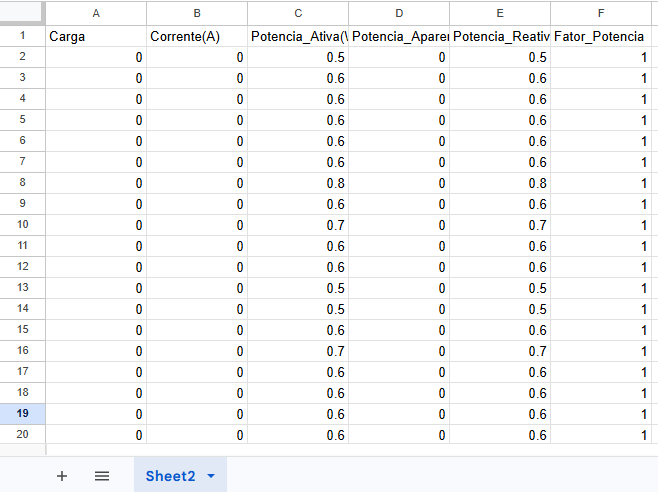
\includegraphics[width=\textwidth]{Figuras/Base de Dados - sheet2.png}
    \label{fig:planilha_dados_class}
    \fonte{\me{2026}}
\end{figure}

\begin{figure}[!htbp]
    \centering
    \caption{Visualização parcial da planilha de dados experimentais para o modelo de Regressão.}
    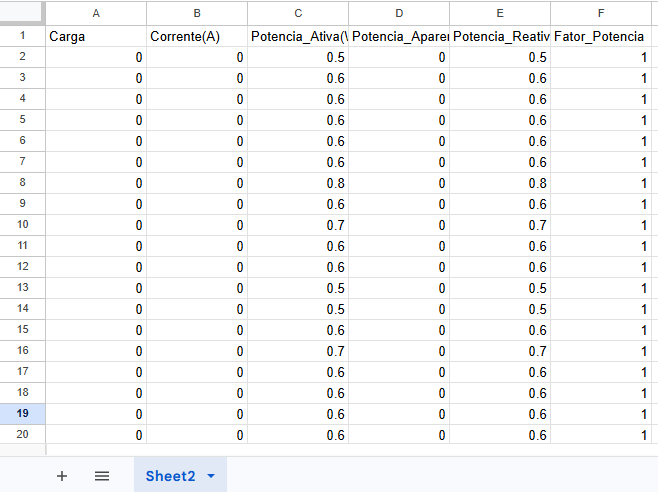
\includegraphics[width=\textwidth]{Figuras/Base de Dados - sheet2.png}
    \label{fig:planilha_dados_reg}
    \fonte{\me{2026}}
\end{figure}

As planilhas completas pode ser acessadas publicamente por meio do link:
\textbf{\url{https://drive.google.com/drive/folders/1i04sDnp_ZCUW4ox6y58tLU4OqA8bNqsv?usp=sharing}}


% ----------------------------------------------------------
% ----------------------------------------------------------
% APÊNDICE D - Código de integração entre o sensor PZEM-004T e o NodeMCU
% ----------------------------------------------------------
\chapter{Código de integração entre o sensor PZEM-004T e o Node MCU}
\label{apendice_integracao_PZEM_MQTT}

Código implementado em C++ para integração entre as medições do sensor PZEM-004T ao MQTT.

\begin{lstlisting}[language=C++, caption={Integração entre PZEM e MQTT.}, label=cod_integracao_PZEM_MQTT]
/*
===================================================================
Autor: Hirislayne Batista Ramos dos Santos
===================================================================
*/

#include <Arduino.h>
#include <PZEM004Tv30.h>
#include <ESP8266WiFi.h>
#include <PubSubClient.h>
#include <NTPClient.h>
#include <WiFiUdp.h>

#define BUILTIN_LED 2

// USANDO A SERIAL PADRÃO (GPIO1 E GPIO3) - NÃO USA SOFTWARE SERIAL!
PZEM004Tv30 pzem(Serial);  // PZEM nos pinos 1(TX) e 3(RX)

// Configurações de Rede e MQTT
const char* ssid = "NOME_RED_WIFI";
const char* password = "SENHA_REDE_WIFI";
const char* mqtt_server = "IP_REDE";
const char *mqtt_username = "tcc_hiris";
const char *mqtt_password = "tcc_hiris";

WiFiClient espClient;
PubSubClient client(espClient);
long lastMsg = 0;
char msg[200];

// Configuração do NTP
WiFiUDP ntpUDP;
NTPClient timeClient(ntpUDP, "a.st1.ntp.br", -3 * 3600, 60000); // -3 para Brasil

// Variáveis globais
float voltage = 0;
float current = 0;
float power = 0;
float energy = 0;
float frequency = 0;
float pf = 0;
float apparent = 0;
float reactive = 0;

void setup_wifi() {
  delay(10);
  // Sem debug, não podemos ver mensagens
  WiFi.begin(ssid, password);
  while (WiFi.status() != WL_CONNECTED) {
    delay(500);
    // Sem debug
  }
  randomSeed(micros());
}

void callback(char* topic, byte* payload, unsigned int length) {
  if ((char)payload[0] == '1') {
    digitalWrite(BUILTIN_LED, HIGH);
  } else {
    digitalWrite(BUILTIN_LED, LOW);
  }
}

void reconnect() {
  while (!client.connected()) {
    String clientId = "ESP8266Client-";
    clientId += String(random(0xffff), HEX);
    
    if (client.connect(clientId.c_str(), mqtt_username, mqtt_password)) {
      client.publish("status", "conectado!");
      client.subscribe("status");
    } else {
      delay(5000);
    }
  }
}

void setup() {
  // NÃO inicialize Serial.begin() - isso atrapalharia o PZEM!
  pinMode(BUILTIN_LED, OUTPUT);
  digitalWrite(BUILTIN_LED, LOW);
  
  setup_wifi();
  client.setServer(mqtt_server, 1883);
  client.setCallback(callback);
}

void loop() {
  if (!client.connected()) {
    reconnect();
  }
  client.loop();

  // Atualiza o horário
  timeClient.update();
  
  // Lê os dados do PZEM
  voltage = pzem.voltage();
  current = pzem.current();
  power = pzem.power();
  energy = pzem.energy();
  frequency = pzem.frequency();
  pf = pzem.pf();
  
  if(!isnan(voltage) && !isnan(current) && !isnan(power) && 
     !isnan(energy) && !isnan(frequency) && !isnan(pf)) {
    
    apparent = voltage * current;
    reactive = sqrt(abs(apparent * apparent - power * power));
    if (pf < 0) reactive = -reactive;
    
    long now = millis();
    if (now - lastMsg > 1000) {
      lastMsg = now;

      // Timestamp real
      unsigned long epochTime = timeClient.getEpochTime();
      String formattedTime = timeClient.getFormattedTime();
    
      // Criar um objeto JSON com todos os dados
      String payload = "{";
      payload += "\"tensao\":" + String(voltage) + ",";
      payload += "\"corrente\":" + String(current) + ",";
      payload += "\"potencia\":" + String(power) + ",";
      payload += "\"aparente\":" + String(apparent) + ",";
      payload += "\"reativa\":" + String(reactive) + ",";
      payload += "\"energia\":" + String(energy) + ",";
      payload += "\"frequencia\":" + String(frequency) + ",";
      payload += "\"fp\":" + String(pf) + ",";      
      payload += "\"timestamp\":" + String(epochTime) + ",";        // Unix timestamp
      payload += "\"hora\":\"" + formattedTime + "\",";             // Hora formatada
      payload += "\"timestamp_ms\":" + String(millis());            // ms desde boot
      payload += "}";
      
      // Publicar tudo em um único tópico
      client.publish("pzem/dados", payload.c_str());

      // Publicar os tópicos individuais
      snprintf(msg, 50, "%f", voltage);
      client.publish("tensao", msg);
      
      snprintf(msg, 50, "%f", current);
      client.publish("corrente", msg);
      
      snprintf(msg, 50, "%f", power);
      client.publish("potencia", msg);
      
      snprintf(msg, 50, "%f", apparent);
      client.publish("aparente", msg);
      
      snprintf(msg, 50, "%f", reactive);
      client.publish("reativa", msg);
      
      snprintf(msg, 50, "%f", energy);
      client.publish("energia", msg);
      
      snprintf(msg, 50, "%f", frequency);
      client.publish("frequencia", msg);
      
      snprintf(msg, 50, "%f", pf);
      client.publish("fp", msg);
      
    }
  }
  
  delay(1000);
}

\end{lstlisting}


% ----------------------------------------------------------
% ----------------------------------------------------------
% APÊNDICE E - Código da Análise da base de dados do PZEM
% ----------------------------------------------------------

\chapter{Código de Análise da Base de dados do PZEM}
\label{apendice_análise_PZEM}

Código implementado em Python utilizado na análise exploratória da base de dados coletada com o sensor PZEM-004T para ler o arquivo CSV com as medições e gerar um gráfico de dispersão que ilustra a relação entre corrente elétrica e potência ativa, destacando os agrupamentos correspondentes a cada tipo de carga.

\begin{lstlisting}[language=python, caption={Análise exploratória da base de dados do PZEM-004T.}, label=cod_analise_base_dados_pzem]
# ================================================================
# Autor: Hirislayne Batista Ramos dos Santos
# ================================================================

import pandas as pd
import matplotlib.pyplot as plt
import seaborn as sns
import numpy as np

df = pd.read_csv("/content/PZEM_dados - Sheet2.csv")

# Mapeamento das cargas
carga_map = {
    0: "Sem carga",
    1: "Capacitiva",
    2: "Indutiva",
    3: "Resistiva",
    4: "Motor",
    5: "Resistiva + Capacitiva",
    6: "Resistiva + Indutiva",
    7: "Capacitiva + Indutiva"
}

# Criar gráfico
plt.figure(figsize=(10, 6))

# Plotar cada carga
cargas = sorted(df['Carga'].unique())
cores = plt.cm.tab10(np.linspace(0, 1, len(cargas)))

for carga, cor in zip(cargas, cores):
    subset = df[df['Carga'] == carga]
    plt.scatter(subset['Corrente(A)'], 
               subset['Potencia_Ativa(W)'],
               color=cor, 
               label=carga_map[carga],
               alpha=0.6,
               s=25)

plt.xlabel('Corrente (A)', fontsize=12)
plt.ylabel('Potência Ativa (W)', fontsize=12)
plt.title('Corrente vs Potência Ativa por Tipo de Carga', fontsize=12)
plt.grid(True, linestyle='--', alpha=0.7)
plt.legend(title='Tipo de Carga', loc='upper left', fontsize=10)
plt.tight_layout()
plt.savefig('disp_corrente_potencia.png', dpi=300)
plt.show()

\end{lstlisting}

\end{apendicesenv}


% ----------------------------------------------------------
% ----------------------------------------------------------
% APÊNDICE F - Código da Análise descritiva da Base UCI
% ----------------------------------------------------------
% \chapter{Código de Análise da Base de dados da UCI}
% \label{apendice_análise_UCI}

% Código implementado em Python utilizado na análise exploratória da base UCI para realizar o pré-processamento dos dados, calcular o fator de potência e gerar as análises estatísticas e gráficos apresentados no Capítulo \ref{Resultados e Discussão}.

% \begin{lstlisting}[language=python, caption={Análise da Base de dados da UCI.}, label=cod_análise_base_dados_UCI]
% #  =============================================================
% #  Autor: Hirislayne Batista Ramos dos Santos
% #  =============================================================
% import pandas as pd
% import numpy as np
% import matplotlib.pyplot as plt
% import seaborn as sns
% import matplotlib.dates as mdates

% # ------- PRÉ-PROCESSAMENTO E ANÁLISE INICIAL ----
% # ---- Carregamento das Bases de dados - ano 2010 -------
% file_path = '/content/New_household_power_consumption_2010.csv'
% df= pd.read_csv(file_path, sep=',')
% df.head(5)
% df["Datetime"] = pd.to_datetime(df["Date"] + " " + df["Time"], format="mixed")
% df.set_index('Datetime', inplace=True)
% df.drop(['Date', 'Time'], axis=1, inplace=True)

% # ---- Informações gerais ----
% df.info()
% df.describe()

% # ----- Limpeza de valores ausentes por coluna ----
% print(df.isna().sum())
% df = df.dropna()
% print(df.isna().sum())

% # ---- Cálculo do FP -----
% df["Apparent_power"] = np.sqrt(df["Global_active_power"]**2 + df["Global_reactive_power"]**2)
% df["Power_factor"] = df["Global_active_power"] / df["Apparent_power"]
% df['Power_factor'] = df['Power_factor'].fillna(1.0) # Como podem haver divisões por zero (quando o consumo é 0), preenchemos com 1.0 (eficiência perfeita)


% # -------- ANÁLISES ----------
% # ------ Estatística do FP -----
% print("\nEstatísticas descritivas do Fator de Potência:")
% print(df["Power_factor"].describe())

% # ------Sazonalidade mensal do FP -----
% monthly_fp = df["Power_factor"].resample("M").mean()

% print("\n--- FP médio por mês ---")
% print(monthly_fp)

% # Criando a figura com tamanho adequado
% plt.figure(figsize=(12, 6))

% # Plot com marcadores para destacar os pontos
% plt.plot(monthly_fp.index, monthly_fp.values, 
%          marker='o',           # Adiciona marcadores circulares
%          linestyle='-',        # Linha sólida
%          linewidth=2,          # Espessura da linha
%          markersize=6,         # Tamanho dos marcadores
%          color='royalblue',    # Cor mais profissional
%          markerfacecolor='white',  # Marcador com centro branco
%          markeredgewidth=1.5,  # Borda do marcador
%          markeredgecolor='royalblue')  # Cor da borda

% # Configuração das grades (sua solicitação principal)
% plt.grid(True, which='major', linestyle='--', linewidth=0.5, alpha=0.7)
% plt.grid(True, which='minor', linestyle=':', linewidth=0.3, alpha=0.4)  # Grade menor opcional
% plt.minorticks_on()  # Ativa os ticks menores para a grade menor

% # Melhorando o eixo X (datas)
% plt.gca().xaxis.set_major_formatter(mdates.DateFormatter('%b/%Y'))  # Formato: Mês/Ano
% plt.gca().xaxis.set_major_locator(mdates.MonthLocator())  # Tick a cada mês

% # Título e labels com fontes maiores
% plt.title("Sazonalidade Mensal do Fator de Potência", pad=20)
% plt.xlabel("Mês/Ano")
% plt.ylabel("FP Médio")

% # Ajustes dos eixos
% plt.xticks(rotation=45, fontsize=10)
% plt.yticks(fontsize=10)

% # Adicionar linha de referência (limite mínimo ideal - exemplo)
% plt.axhline(y=0.92, color='red', linestyle='--', linewidth=1, alpha=0.7, label='Limite ideal (0.92)')

% # Adicionar valores nos pontos (opcional - comentado pois pode poluir)
% # for i, (x, y) in enumerate(zip(monthly_fp.index, monthly_fp.values)):
% #     plt.annotate(f'{y:.3f}', (x, y), textcoords="offset points", xytext=(0,10), ha='center', fontsize=8)

% # Limites do eixo Y (ajuste conforme seus dados)
% plt.ylim(0.85, 1.0)  # Ajuste baseado em valores típicos de FP

% # Legenda (se adicionar elementos como a linha de limite)
% plt.legend(loc='best', fontsize=10)

% # Layout ajustado
% plt.tight_layout()

% # Salvar a figura (opcional)
% # plt.savefig('sazonalidade_fp.png', dpi=300, bbox_inches='tight')

% plt.show()

% # ------- Correlação entre as variáveis --------
% cols = [
%     'Global_active_power', 'Global_reactive_power', 'Voltage',
%     'Global_intensity', 'Sub_metering_1', 'Sub_metering_2', 'Sub_metering_3',
%     "Apparent_power", "Power_factor"
% ]

% matriz_correlacao = df[cols].corr()

% plt.figure(figsize=(12, 8))
% sns.heatmap(matriz_correlacao, annot=True, cmap='RdBu', fmt=".2f", vmin=-1, vmax=1)
% plt.title("Mapa de Calor: Correlação entre Variáveis de Consumo")
% plt.show()

% # ------- Relações I, P, Q vs FP ----------
% plt.figure(figsize=(10, 6))
% sns.scatterplot(data=df.sample(min(2000, len(df))), x='Global_active_power', y='Power_factor', alpha=0.5, color="blue")
% plt.title('Relação Potência Ativa vs Fator de Potência')
% plt.xlabel('Potência Ativa (kW)')
% plt.ylabel('Fator de Potência')
% plt.grid(True, linestyle='--', alpha=0.7)
% plt.show()

% plt.figure(figsize=(10, 6))
% sns.scatterplot(data=df.sample(min(2000, len(df))), x='Global_intensity', y='Power_factor', alpha=0.5, color="orange")
% plt.title('Relação Corrente vs Fator de Potência')
% plt.xlabel('Corrente (A)')
% plt.ylabel('Fator de Potência')
% plt.grid(True, linestyle='--', alpha=0.7)
% plt.show()

% plt.figure(figsize=(10, 6))
% sns.scatterplot(data=df.sample(min(2000, len(df))), x='Global_reactive_power', y='Power_factor', alpha=0.5, color="green")
% plt.title('Relação Potência Reativa vs Fator de Potência')
% plt.xlabel('Potência Reativa (kVAr)')
% plt.ylabel('Fator de Potência')
% plt.grid(True, linestyle='--', alpha=0.7)
% plt.show()

% # ------- Periodo de ocorrencia dos menores FP ------------
% df['Hour'] = df.index.hour
% threshold_low = df["Power_factor"].quantile(0.01)
% lowest_fp = df[df["Power_factor"] <= threshold_low]

% print("Limite do 1% menor FP:", threshold_low)
% print("\nResumo estatístico dos menores FPs:")
% print(lowest_fp["Power_factor"].describe())

% print("\nDistribuição por hora (menores FPs):")
% print(lowest_fp["Hour"].value_counts().sort_index())

% # Gráfico melhorado
% plt.figure(figsize=(12, 6))

% # Histograma com bordas e cores
% counts, bins, patches = plt.hist(lowest_fp["Hour"], 
%                                  bins=24, 
%                                  range=(0, 24),
%                                  edgecolor='black', 
%                                  linewidth=1.2,
%                                  alpha=0.7,
%                                  color='steelblue')

% # Adicionar grades
% plt.grid(True, linestyle='--', alpha=0.6, axis='y')
% plt.grid(True, linestyle=':', alpha=0.3, axis='x', which='minor')

% # Configurações dos eixos
% plt.xticks(np.arange(0, 24, 2))
% plt.xticks(np.arange(0, 24, 1), minor=True)
% plt.xlabel("Hora do Dia")
% plt.ylabel("Frequência (Número de Ocorrências)")
% plt.title("Distribuição Horária dos 1% Menores Fatores de Potência", pad=15)

% # Adicionar linha de média
% plt.axhline(y=counts.mean(), color='red', linestyle='--', 
%             linewidth=1.5, alpha=0.7, label=f'Média: {counts.mean():.1f}')

% # Destacar pico
% max_idx = np.argmax(counts)
% plt.annotate(f'Pico: {int(counts[max_idx])}', 
%              xy=(bins[max_idx] + 0.5, counts[max_idx]), 
%              xytext=(bins[max_idx] + 2, counts[max_idx] + 2),
%              arrowprops=dict(arrowstyle='->', color='darkred'),
%              fontsize=10, fontweight='bold', color='darkred')

% # Legenda
% plt.legend(loc='upper right')

% # Ajustes finais
% plt.tight_layout()
% plt.show()

% */

% \end{lstlisting}
				% Elemento Opcional
%\include{PosTextuais/Anexos}				% Elemento Opcional
%\include{PosTextuais/IndiceRemissivo}		% Elemento Opcional

\end{document}